%% Basierend auf einer TeXnicCenter-Vorlage von Mark M�ller
%%%%%%%%%%%%%%%%%%%%%%%%%%%%%%%%%%%%%%%%%%%%%%%%%%%%%%%%%%%%%%%%%%%%%%%

% W�hlen Sie die Optionen aus, indem Sie % vor der Option entfernen  
% Dokumentation des KOMA-Script-Packets: scrguide

%%%%%%%%%%%%%%%%%%%%%%%%%%%%%%%%%%%%%%%%%%%%%%%%%%%%%%%%%%%%%%%%%%%%%%%
%% Optionen zum Layout des Buchs                                     %%
%%%%%%%%%%%%%%%%%%%%%%%%%%%%%%%%%%%%%%%%%%%%%%%%%%%%%%%%%%%%%%%%%%%%%%%
\documentclass[
paper=a4,							% alle weiteren Papierformat einstellbar
%landscape,						% Querformat
12pt,								% Schriftgr��e (12pt, 11pt (Standard))
BCOR=1cm,							% Bindekorrektur, bspw. 1 cm
%DIVcalc,							% f�hrt die Satzspiegelberechnung neu aus
%											  s. scrguide 2.4
%oneside,							% einseitiges Layout
%twocolumn,						% zweispaltiger Satz
%openany,							% Kapitel k�nnen auch auf linken Seiten beginnen
%halfparskip*,				% Absatzformatierung s. scrguide 3.1
headsepline=true,			% Trennline zum Seitenkopf	
%footsepline,					% Trennline zum Seitenfu�
notitlepage,					% in-page-Titel, keine eigene Titelseite
%chapterprefix,				% vor Kapitel�berschrift wird "Kapitel Nummer" gesetzt
%appendixprefix,				% Anhang wird "Anhang" vor die �berschrift gesetzt 
%normalheadings,			% �berschriften etwas kleiner (smallheadings)
%idxtotoc,						% Index im Inhaltsverzeichnis
%liststotoc,					% Abb.- und Tab.verzeichnis im Inhalt
bibliography=totoc,						% Literaturverzeichnis im Inhalt
%leqno,								% Nummerierung von Gleichungen links
%fleqn,								% Ausgabe von Gleichungen linksb�ndig
%draft,								% �berlangen Zeilen in Ausgabe gekennzeichnet
%cleardoubleplain,    % leere, linke Seite mit Seitenstil 'plain' 
%cleardoubleempty,    % leere, linke Seite mit Seitenstil 'empty'
]
{scrbook}

%\pagestyle{empty}		% keine Kopf und Fu�zeile (k. Seitenzahl)
%\pagestyle{headings}	% lebender Kolumnentitel  

%% Deutsche Anpassungen %%%%%%%%%%%%%%%%%%%%%%%%%%%%%%%%%%%%%
\usepackage[ngerman]{babel}
\usepackage[ansinew]{inputenc}
\usepackage[T1]{fontenc}
\usepackage[hypertexnames=false]{hyperref}	% Paket welches die M�glichkeit gibt Links und Verweise innerhalb von PDF Dokumenten zu erzeugen und zu setzen
																						% Ziemlich fr�h Einbinden, sonst werden Abbildungen als Abschnitte via \autoref referenziert.
\usepackage{csquotes}												% Wenn babel verwendet wird mit biblatex, csquotes wird empfohilen zur Darstellung von Anf�hrungszeichen
\usepackage{lmodern} 												% Pixelfreie Schrift
\usepackage{booktabs}												% Tabellen Paket
\usepackage[subfigure]{ccaption}					 
\usepackage{threeparttable} 								% Tabellen Paket um Tabellen mit �berschriften, Fu�noten, ... zu versehen
%\usepackage{a4}	 														% europ�isches A4
\usepackage{courier}												% Stellt Courier New korrekt dar
\usepackage{wasysym}												% Zus�tzliche Symbole wie CheckedBox
\usepackage{marvosym}												% Zus�tzliche Symbole wie CheckedBox
\usepackage{pmboxdraw}											% f�r die Ordnerbaum-Symbole
\usepackage{amssymb} 												% f�r \boxplus und \boxminus
\usepackage{siunitx}												% SI-Einheiten

%% \autoref Name "`Kapitel"' statt "`Unterabschnitt"'
\addto\extrasngerman{%
\def\subsectionautorefname{Kapitel}%
\def\sectionautorefname{Kapitel}%
}

%% Hurenkinder und Schusterjungen verhindern
\clubpenalty10000
\widowpenalty10000
\displaywidowpenalty=10000

%% Packages f�r Grafiken & Abbildungen %%%%%%%%%%%%%%%%%%%%%%
\usepackage{graphicx} %% Zum Laden von Grafiken
\usepackage{subfigure} %% Teilabbildungen in einer Abbildung
\newcommand{\subfigureautorefname}{\figureautorefname} % \autoref Name f�r subfigures
%% Beachten Sie:
%% Die Einbindung einer Grafik erfolgt mit \includegraphics{Dateiname}
%% bzw. �ber den Dialog im Einf�gen-Men�.
%% 
%% Im Modus "LaTeX => PDF" k�nnen Sie u.a. folgende Grafikformate verwenden:
%%   .jpg  .png  .pdf  .mps
%% 
%% In den Modi "LaTeX => DVI", "LaTeX => PS" und "LaTeX => PS => PDF"
%% k�nnen Sie u.a. folgende Grafikformate verwenden:
%%   .eps  .ps  .bmp  .pict  .pntg

%% Bibliographiestil %%%%%%%%%%%%%%%%%%%%%%%%%%%%%%%%%%%%%%%%%%%%%%%%%%
\usepackage[
style=authoryear,
natbib,
dashed=false,									% Bei mehreren Werken eines Autors alle einzeln anzeigen
backend=biber, 
block=space										% kleiner horizontaler Platz zwischen den Feldern
]{biblatex}										% Literaturangaben mit BibTeX
\DeclareNameAlias{sortname}{last-first}
\addbibresource{MasterBib.bib}
\setlength{\bibitemsep}{1em}	% Abstand zwischen den Literaturangaben
\setlength{\bibhang}{2em}   	% Einzug nach jeweils erster Zeile

%% Abk�rzungsverzeichnis %%%%%%%%%%%%%%%%%%%%%%%%%%%%%%%%%%%%%
\usepackage{nomencl}					% Paket f�r Abk�rzungsverzeichnis
\makeindex										% Erstellt Masterarbeit.idx welche f�r das Abk�rzungsverzeichnis n�tig ist
															% Muss zwingend VOR \makenomenclature aufgerufen werden!
\let\abk\nomenclature
\renewcommand{\nomname}{Abk�rzungsverzeichnis}  
\setlength{\nomlabelwidth}{0.20\hsize}			  	% Punkte zw. Abk�rzungen und Beschreibung
\renewcommand{\nomlabel}[1]{#1 \dotfill}				
\setlength{\nomitemsep}{-\parsep}								% Zeilenabst�nde verkleinern
\makenomenclature 

%% Quellcode Listings %%%%%%%%%%%%%%%%%%%%%%%%%%%%%%%%%%%%%
\usepackage{listings}
\usepackage[table, dvipsnames]{xcolor}	
\definecolor{KeilGreen}{RGB}{189,249,181}
\definecolor{mygreen}{rgb}{0,0.6,0}
\definecolor{mygray}{rgb}{0.5,0.5,0.5}
\definecolor{mymauve}{rgb}{0.58,0,0.82}

% Style f�r C++
\lstdefinestyle{customcpp}{
  belowcaptionskip=1\baselineskip,
  breaklines=true,
  frame=none,
  xleftmargin=\parindent,
  language=C,
	numbers=left,                     % where to put the line-numbers; possible values are (none, left, right)
  showstringspaces=false,
	%numberstyle=\tiny,								% the style that is used for the line-numbers 
  basicstyle=\footnotesize\ttfamily,
  keywordstyle=\bfseries\color{blue!40!black},
  commentstyle=\itshape\color{green!40!black},
  identifierstyle=\color{black},
  stringstyle=\color{orange},
}
\renewcommand{\lstlistingname}{Quelltext}	% �nder den Name von "`Listing"' auf Quelltext
\newcommand{\lstnumberautorefname}{Zeile}

% Warning, dass mehrere pdfs auf einer Seite sind unterdr�cken
\pdfsuppresswarningpagegroup=1
\pdfminorversion=7

%%%%%%%%%%%%%%%%%%%%%%%%%%%%%%%%%%%%%%%%%%%%%%%%%%%%%%%%%%%%%%%%%%%%%%%
%% Buch                                                              %%
%%%%%%%%%%%%%%%%%%%%%%%%%%%%%%%%%%%%%%%%%%%%%%%%%%%%%%%%%%%%%%%%%%%%%%%
\begin{document}

%%%%%% Titelseite %%%%%%
\frontmatter						% ab hier r�mische Nummerierung
%Titelseite zentrieren
\newlength\oddsidemarginorig				
\oddsidemarginorig=\oddsidemargin
\advance\oddsidemargin\evensidemargin
\divide\oddsidemargin by 2

%Layout und Text f�r Titelseite
\begin{titlepage}
\begin{center}
\vspace*{0cm}
\hrulefill \\
\vspace*{0.5cm}
\textbf{\LARGE Model Driven Software Engineering \\ mit IBM Rational Rhapsody \\ f�r Embedded Systems \\}	
\vspace*{0.5cm}
%{\bf \huge zum Wintersemester 2012/2013\\}	
\hrulefill \\
\vspace*{1.6cm}
\textbf {\Large Masterprojekt \\}
\vspace*{2cm}
{\large Thomas Sauter \\ Matrikel-Nr.: 3122629\\ Studiengang: SYE\verb|\|2 \\}
\vspace*{1cm}
{\large Hochschule Ulm \\ Graduate School \\ Studiengang Systems Engineering und Management \\}
\vspace*{1cm}
%{\large Firma EvoBus GmbH in Neu-Ulm\\}
\vspace*{1cm}
\textbf{\Large \today \\}
\end{center}
\vspace*{\fill}
\noindent \underline{Betreuer:} \\
																Prof. Dr. Marianne von Schwerin, Hochschule Ulm \\

\end{titlepage}

\cleardoublepage				% mit neuer ungerader Seite weiter

%%%%%% Inhaltsverzeichnis %%%%%%
\tableofcontents				% Inhaltsverzeichnis
\cleardoubleoddpage			% Sorgt daf�r, dass die �nderung der Seitennummerierung
												% immer auf einer neuen (rechten) Seite beginnt!
\mainmatter							% ab hier arabische Nummerierung

%% Der Text %%%%%%%%%%%%%%%%%%%%%%%%%%%%%%%%%%%%%%%%%%%%%%%%%%%%%%%%%%%
\chapter{Einleitung}

\section{Motivation}

Das Programmieren von Software kann derzeit in vier Generationen eingestuft werden \parencite{ModelingEmbeddedSystems}. Dabei repr�sentiert die erste Generation die Maschinensprache. Zwar findet die Maschinensprache noch heute Anwendung in allen Prozessoren, allerdings ist das Schreiben von Maschinensprache als bin�rer oder hexadezimaler Code �u�erst m�hselig und fehleranf�llig. 

Deshalb wurde mit der zweiten Generation die Assemblersprache eingef�hrt. Dabei �bersetzt ein Computerprogramm, der Assembler, die Assemblersprache in Maschinensprache. Einheitliche Befehle in Textform erm�glichen ein schnelleres und besser Verst�ndnis daf�r, was ein Programm tats�chlich ausf�hrt. Fehler k�nnen dennoch vorkommen, allerdings nicht mehr in einfachen Konstrukten.Schlie�lich wurden die Programme in Assemblersprache mit zunehmender Dauer gr��er und un�bersichtlicher, wodurch deren Wartung und Test immer schwerer wurde. 

Die h�heren Programmiersprachen wie C oder C++ l�uteten daraufhin die dritte Generation ein, die bis heute Verwendung findet. Die abstrakte Syntax ist eher an menschliche Gewohnheiten angepasst und beschreibt, wie ein Problem gel�st wird. Ein Compiler �bersetzt den Quellcode in Maschinensprache. Aber auch hier w�chst die Software kontinuierlich, wodurch erneut das Problem der Komplexit�t auftritt. Das spiegelt sich auch in einer Umfrage von \citet[Folie 48]{EmbeddedMarketsStudy} wider. Dort wird die steigende Komplexit�t, verbunden mit der zunehmenden Anzahl an Codezeilen, als gr��te Herausforderungen im kommenden Jahr in der Entwicklung von Software f�r Embedded Systems angegeben.

Abhilfe sollen die Sprachen der vierten Generation schaffen, wobei die Literatur die Inhalte der vierten Generation nicht klar abgrenzt. Nach \citet{ModelingEmbeddedSystems} geh�rt zur vierten Generation auch die Modellierungssprache UML. Die UML hebt die Programmierung nochmals auf eine h�here Abstraktionsebene und versucht so die Komplexit�t zu bew�ltigen. Dabei kommen standardisierte Modellelemente zum Einsatz, die eine h�here Informationsdichte haben als �bliche Programmiersprachen. Mit den Modellelementen k�nnen Grafiken wie Klassen-, Sequenz- und Zustandsdiagramme modelliert werden. Oft ist es noch g�ngige Praxis, dass UML-Modelle lediglich zur Dokumentation verwendet werden. Dabei wird aber nicht das gesamte Potential der UML ausgenutzt. Zusammen mit einem Codegenerator entwickelt sich die UML zu einer leistungsstarken Modellierungssprache, bei der das Programmieren vom Modellieren abgel�st wird. In diesem Zusammenhang ist eine Entwicklungsumgebung, welche das automatisierte Generieren von Quellcode unterst�tzt, unverzichtbar. Bezogen auf die vier Generationen �berf�hrt der Codegenerator das UML-Modell aus der vierten Generation in ausf�hrbaren Quellcode der dritten Generation.     

\section{Aufgabenstellung}

Der Fokus im Rahmen dieser Arbeit liegt auf der modellbasierten Softwareentwicklung f�r Embedded Systems. Die Basis bildet die Laborveranstaltung zur Vorlesung Embedded Systems. Dort wurde bisher mit Hilfe des Tools IBM Rational Rhapsody und des Willert Realtime RXF aus UML-Modellen Quellcode in C generiert. Der generierte Quellcode wird in der Entwicklungsumgebung Keil uVision kompiliert und auf ein Evaluierungsboard geladen. 

Die erste Aufgabe besteht darin, die bisher existierenden Laboraufgaben von der Programmiersprache C nach C++ zu �berf�hren. Besonderheiten in diesem Zusammenhang stellt das Einbinden externer C-Quellen dar, was im Weiteren Verlauf der Arbeit nochmals thematisiert wird. L�sungen der Laboraufgaben in der Programmiersprache C++ sind nicht Inhalt der vorliegenden Arbeit.

In den existierenden Laboraufgaben wurden bereits verschiedene Peripherieger�te des Evaluierungsboards verwendet, unter anderem LED-Bar, Poti, Display, Joystick und Interrupt-Button. Hier sollen weitere Bauteile angesprochen und die Laboraufgaben erweitert werden. Dabei handelt es sich um folgende Funktionalit�ten:

\begin{itemize}
\item Ethernet-Kommunikation
\item WLAN-Kommunikation
\item Lesen und Schreiben einer SD-Karte
\end{itemize}

Das Hauptaugenmerk bei der Implementierung liegt darauf, dass der generierte C++-Quellcode in Keil uVision nicht mehr ge�ndert werden muss, ansonsten geht der Vorteil der automatisierten Codegenerierung durch Rational Rhapsody verloren. Eine Ausnahme bildet die WLAN-Kommunikation. Da das Evaluierungsboard �ber keine eigene WLAN-Antenne verf�gt, muss diese �ber einen externes WLAN-Modul zur Verf�gung gestellt werden. Zwar erfolgt die Implementierung f�r das Evaluierungsboard �ber die bestehende Toolkette, jedoch ben�tigt das externe WLAN-Modul eine spezifische Entwicklungsumgebung in welcher der entsprechende Code von Hand implementiert wird.

Den Abschluss der Arbeit bildet die Verifikation. Dabei soll auch ein modellbasierter Test implementiert werden. Rational Rhapsody bietet dazu die Erweiterung TestConductor an, welche diese Funktionalit�t unterst�tzt. Damit aus den modellierten Testf�llen ausf�hrbarer Quellcode entstehen kann, wird ebenfalls das Willert Realtime RXF sowie Keil uVision ben�tigt. Zu Beginn der Arbeit war geplant, dass die Implementierungen zu den neuen Funktionen einem modellbasierten Test unterzogen werden. Allerdings existiert derzeit kein Willert Realtime RXF, das die verwendete Toolchain und den TestConductor unterst�tzt, sowie C++-Quellcode generiert. Ein Release eines entsprechenden Willert Realtime RXF ist f�r das vierte Quartal im Jahr 2017 vorgesehen. Aus diesem Grund soll eine der bereits existierenden Laboraufgaben in C verwendet werden und exemplarisch ein Testszenario modelliert werden.

\chapter{Entwicklungsumgebung}

\section{Hardware}

\subsection{Evaluation Board Keil MCB1760}
Das Keil MCB1760 Evaluation Board enth�lt einen NXP LPC1768 Mikrocontroller basierend auf einem  100Mhz ARM 32-bit Cortex-M3 Mikroprozessor. Neben den wesentlichen Komponenten und Schnittstellen, welche in \autoref{fig:MCB1760EvalBoard} dargestellt sind, verf�gt das Keil MCB1760 Evaluation Board �ber 512KB Flash und 64KB RAM Speicher.

\begin{figure}[ht!]
	\centering
	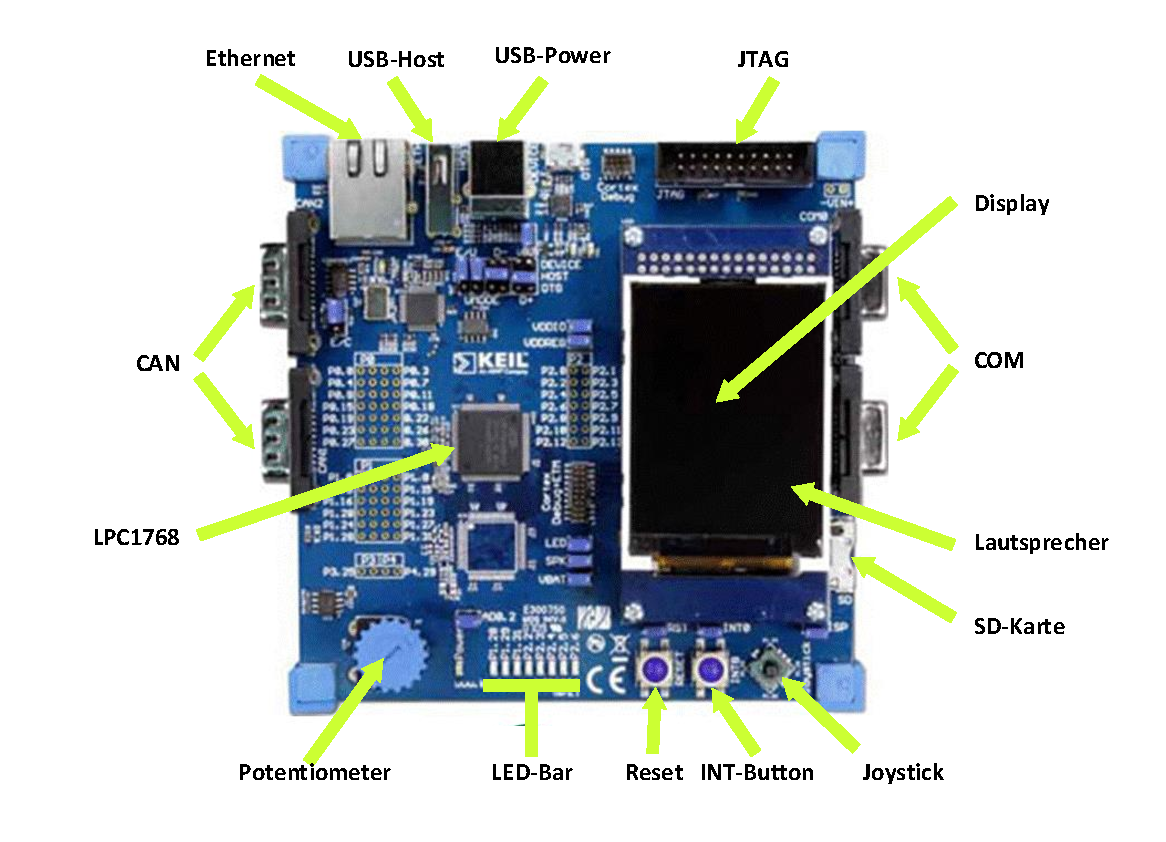
\includegraphics[width=1\textwidth]{images/MCB1700.pdf}
	\caption{Komponenten des MCB1760 Evaluation Board.}
	\label{fig:MCB1760EvalBoard}
\end{figure}

In der Regel werden Evaluation Boards in fr�heren Entwicklungsphasen eingesetzt, um die Leistungsgrenzen der gew�hlten Architektur zu verifizieren. Im Rahmen dieser Arbeit steht die Integration des Evaluation Boards zusammen mit der Toolchain im Vordergrund. 

\subsection{WLAN-Modul ESP8266}

\begin{figure}[b!]
	\centering
		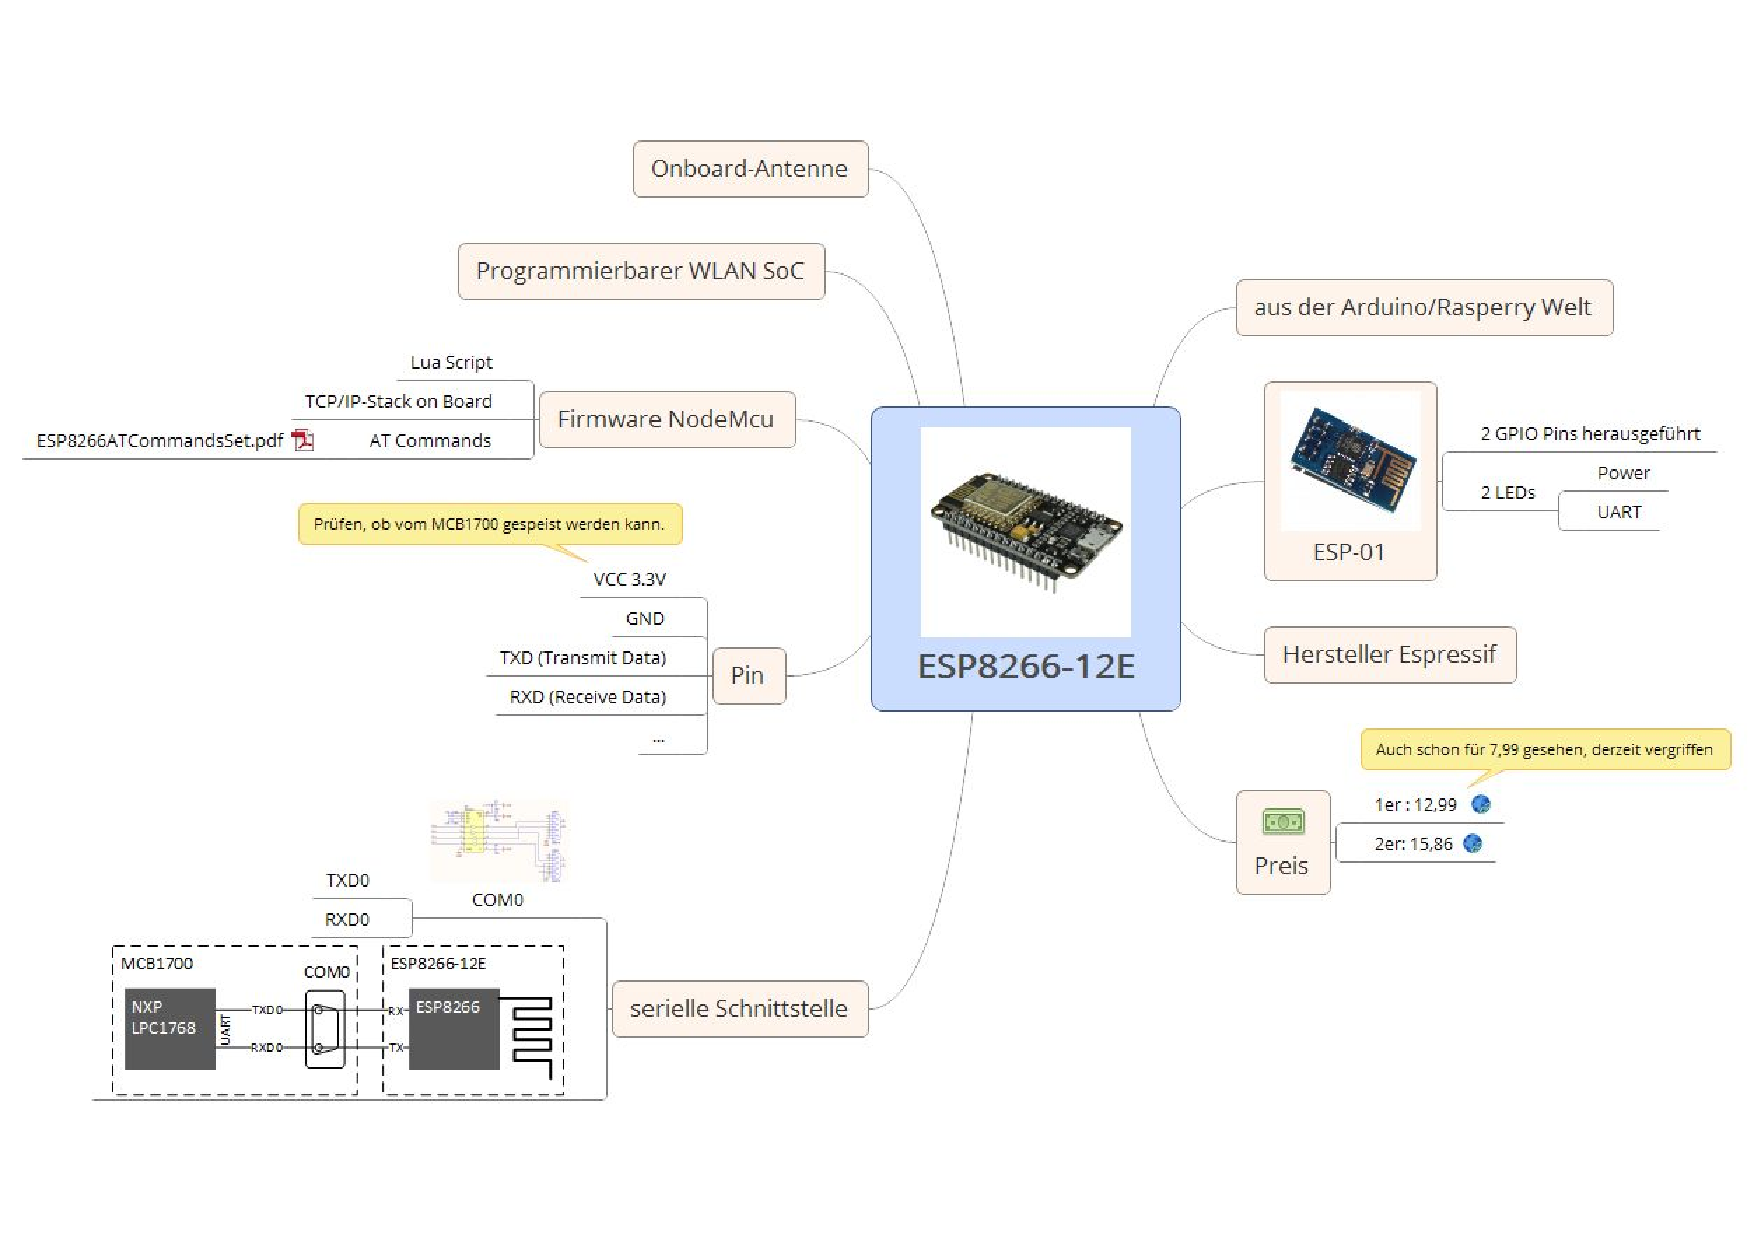
\includegraphics[width=1\textwidth]{images/ESP8266_E12.pdf}
		\caption{WLAN-Modul ESP8266.}
	\label{fig:ESP8266}
\end{figure}

Das WLAN-Modul ESP8266 ist eines von wenigen Boards auf dem Markt, das �ber einen Mikrocontroller mit WLAN-Funktionalit�t verf�gt. Das Herzst�ck des Mikrocontrollers ist der bis zu 160MHz schnelle 32-bit Xtensa LX106 Mikroprozessor von Tensilica. Dabei gibt eine ganze Reihe von Boards, die sich vor allem in ihrer Dimension, den damit zug�nglichen Pins und dem Flash Speicher unterscheiden. Im Rahmen dieser Arbeit wird das Board ESP8266-12E verwendet, wie es in \autoref{fig:ESP8266} dargestellt ist. Das Board verf�gt �ber 4MB Flash und 65KB RAM Speicher. Eine hohe Popularit�t im Internet erlangte das Board auch unter dem Begriff \textit{NodeMCU}. Der Name \textit{NodeMCU} stammt dabei von der Firmware, die ab Werk vorinstalliert ist. Die Open-Source Firmware basiert auf der Skriptsprache Lua. In dieser Arbeit wird die Firmware \textit{NodeMCU} nicht verwendet, weshalb das Board im Weiteren auch als WLAN-Modul ESP8266 bezeichnet wird. Die Programmierung �ber Lua-Skripte ist m�glicherweise komfortabler, bietet aber eine wesentlich geringere Flexibilit�t als eine Programmiersprache wie C. 

Der gro�e Vorteil des verwendeten Boards liegt in der USB-Schnittstelle. Diese dient als Programmier-Schnittstelle und Spannungsversorgung zugleich.  Dabei wird die USB-Schnittstelle durch den USB/UART-Wandler CH340G und eine Spannungsstabilisierung unterst�tzt. Das vereinfacht die Programmierung des ESP8266, da nicht beachtet werden muss, dass bestimmte Pins vor der Programmierung definierte Pegel haben. Zudem muss keine explizite Spannungsversorgung entwickelt werden. 

\section{Software}

\subsection{IBM Rational Rhapsody}

Derzeit gibt es auf dem Markt eine Vielzahl an Software-Modellierungswerkzeuge, die sich im Wesentlichen durch ihre Funktionen und den daraus resultierenden Preis unterscheiden. Jedoch haben die meisten dieser Tools miteinander gemein, dass sie die Modellierungssprache UML unterst�tzen. So gibt es unter anderem einige kostenlose Tools wie StarUML oder Netbeans, die geringen Anforderungen durchaus gen�gen. Weitaus m�chtiger sind etwa Enterprise Architect von SparxSystems und das in dieser Arbeit verwendete Rational Rhapsody von IBM. Mit Rational Rhapsody ist es m�glich, nebem UML-Modellierung weitere Aufgaben zu bearbeiten, die w�hrend der Softwareentwicklung anfallen. Beispielsweise k�nnen Anforderungen direkt spezifiziert oder auch aus DOORS NG importiert und zu der erstellten Architektur verlinkt werden. Ein Codegenerator �bersetzt die Architektur in Quelltext. Dabei bietet der Codegenerator etliche Konfigurationsm�glichkeiten, um Layout und Syntax nach Belieben anzupassen. Das Spezifizieren und Ausf�hren von Tests in einer integrierten Testumgebung runden den Funktionsumfang zur Unterst�tzung eines Software Entwicklungsprozesses ab.

Rational Rhapsody wird in verschiedenen Versionen Angeboten, die sich stark in ihrem Funktionsumfang unterscheiden. Grundlegende Funktionen, wie etwa das Erstellen von UML-Diagrammen und das Verlinken von Anforderungen ist mit allen Versionen m�glich. Weitere Funktionalit�ten wie grafikbasierte Simulation oder  
automatische Codegenerierung, unter anderem auch f�r Embedded Echtzeitsysteme, ist nur in den Premium-Versionen verf�gbar \parencite{IBM2017}. 

Beim Generieren von Quelltext unterst�tzt Rational Rhapsody die Programmiersprachen C, C++, Java und C\#. Dabei ist es wichtig, dass direkt beim Anlegen des Projekts die gew�nschte Programmiersprache ausgew�hlt wird. Denn in der Folge startet Ratioal Rhapsody beim �ffnen der Rhapsody Projektdatei stets die passende Variante f�r die definierte Programmiersprache. Da die Implementierungen in dieser Arbeit in C++ erfolgen, ergibt sich somit die Version \textit{IBM Rational Rhapsody Developer for C++}, die zudem den vollen Funktionsumfang beinhaltet. 

\subsubsection*{Rhapsody TestConductor Add On}

Der Rhapsody TestConductor ist Teil der Testumgebung von Rational Rhapsody, welche auf drei Hauptkomponenten basiert:

\begin{itemize}
\item Automatisiertes Generieren von Test-Architekturen
\item Automatisiertes Generieren von Testf�llen
\item Automatisiertes Ausf�hren von Testf�llen
\end{itemize}

Dabei unterst�tzt der TestConductor in der Basisversion das automatisierte Generieren von Test-Architekturen, sowie das Ausf�hren von Testf�llen. Mit der Erweiterung Automatic Test Generation (ATG) wird auch das automatisierte Generieren von Testf�llen unterst�tzt. Ungeachtet dessen steht im Fokus des TestConductors der modellbasierte, dynamische Test. So erm�glicht der TestConductors das Modellieren von Testf�llen in Form von Sequenz-, Zustands- und Aktivit�tsdiagrammen. Zus�tzlich ist es aber auch m�glich, Testf�lle als Quellcode zu implementieren.

Dar�ber hinaus bringt der TestConductor das Rhapsody UML Testing Profile mit sich, basierend auf dem offiziellen UML Testing Profile der \citet{OMGUMLTestingProfile}. Dabei gilt es zu beachten, dass das Rhapsodoy UML Testing Profile nicht alle Elemente des UML Testing Profiles enth�lt. Aber es verf�gt �ber zus�tzliche Elemente, die nicht Teil des UML Testing Profiles der OMG sind. Ein Beispiel daf�r sind Platzhalter f�r Schnittstellen, die nicht Teil der zu testenden Komponente sind \parencite{TestConductorAddOn}. 

\subsection{Willert Embedded UML RXF}
Der generierte Code aus Rhapsody eignet sich zun�chst nicht zur Ausf�hrung auf einem Target. Die UML-Notation ist viel leistungsst�rker und auf einer h�heren Abstraktionsebene als jede h�here Programmiersprache. UML-Elemente wie asynchrone Kommunikation, aktive Klassen oder auch komplexe Zust�nde k�nnen nicht direkt in eine h�here Programmiersprache �bersetzt werden. 

Das Tool Embedded UML Real-time eXecution Framework (RXF)\abk{$RXF$}{Real-time eXecution Framework} der Firma Willert bildet die Schnittstelle zwischen UML-Modell und einer Zielplattform bestehend aus Compiler, CPU\abk{$CPU$}{Central Processing Unit} und einem m�glichen RTOS\abk{$RTOS$}{Real Time Operating System}. Durch eine Abstraktionsschicht werden die g�ngigsten Echtzeit-Betriebssysteme auf dem Markt unterst�tzt. Das bedeutet, dass in UML definierte Timer oder Events unabh�ngig vom Betriebssystem verwendet werden k�nnen. Somit ist das Software-Design komplett losgel�st vom gew�hlten Target.

Bei der Codegenerierung unterst�tzt das RXF die beiden bekanntesten UML-Tools, Rhapsody und Sparx Enterprise Architect, sowie eine Vielzahl an IDEs\abk{$IDE$}{Integrated Development Environment}. Um eine bestm�gliche Integration zu gew�hrleisten, ist jede Variante des RXF auf die verwendete Toolchain zugeschnitten. Ein Vorteil davon ist, dass die Target IDE �ber das RXF mit Rhapsody verbunden ist und somit der Code aus dem UML-Modell direkt in die Target IDE generiert wird \parencite{ModelingEmSys}. Zur Unterscheidung der vielen verschiedenen Varianten hat die Firma Willert mit der Version 6 einen Produktcode eingef�hrt, welcher zur Identifikation der enthaltenen Komponenten dient. Das Schema ist in \autoref{tab:WillertProduktcode} abgebildet.

\begin{table}[!b]
\centering
\small
	\begin{threeparttable}
	\begin{tabular}{c|c|c|c|c|c}
		\toprule
			 UML-Tool & Programmiersprache & RTOS & Compiler & EvalBoard\tnote{*} & Erweiterungen\tnote{**}\hspace{1ex} \\
		\bottomrule
		\end{tabular}
		\begin{tablenotes}
			\footnotesize 
			\item[*]{Die EvalBoard Komponente ist kein Teil des Produkts. Sie sagt lediglich aus, mit welcher CPU Familie das Produkt verwendet werden kann.}
			\item[**]{Erweiterungen sind optional und k�nnen auch miteinander kombiniert werden. M�gliche Zus�tze sind "`TD"' f�r Embedded UML Target Debugger, "`TC"' f�r Test Conductor oder "`Eval"' f�r eine RXF Evaluierungsversion.}
		\end{tablenotes}
	\end{threeparttable}
	\caption{Produktcode zur Identifikation der enthalten Komponenten \parencite{RXFMigrationGuide}.}
	\label{tab:WillertProduktcode}
\end{table}

In dieser Arbeit wurden die Varianten \begin{itshape}RXF-Eval\_Rpy-Cpp-ARM\end{itshape} in der Version 6.02 und \begin{itshape}Rpy\_CPP\_CMSIS\_Keil5\_ARM\_MCB1700\_TD\end{itshape} in der Version 6.01 verwendet.

\subsection{Keil uVision}
Die IDE Keil uVision ist Teil des Keil Microcontroller Development Kit (MDK)\abk{$MDK$}{Microcontroller Development Kit}. Es vereint einen Projektmanager und eine Run-Time Environment (RTE)\abk{$RTE$}{Run-Time-Environment}, mit deren Hilfe vorgefertigte Software Pakete integriert werden k�nnen. Die Software Pakete k�nnen Bibliotheken, Module, Konfigurationsdateien, Templates und Dokumentation enthalten, welche bei der Inbetriebnahme des Targets unterst�tzen. Die Basisfunktionalit�ten einer gew�hnlichen IDE, wie Quellcode-Editor und Debugger, sind ebenfalls enthalten \parencite{MDK}.

In dieser Arbeit wird das Keil MDK in der Version 5 verwendet. Im Vergleich zum vorherigen Keil MDK in der Version 4, ist eine wesentliche Neuerung das Echtzeitbetriebssystem Cortex Microcontroller Software Interface Standard (CMSIS)\abk{$CMSIS$}{Cortex Microcontroller Software Interface Standard}. Es l�st das bisherige RTX Real-Time Library (RL-ARM)\abk{$RL-ARM$}{Real-Time Library for ARM microprocessors} Echtzeitbetriebssystems ab und bringt die folgenden Vorteile mit sich \parencite{RLARMtoCMSIS}: 

\begin{itemize}
\item Standardisierte API
\item Basisfunktionen zur Unterst�tzung von UML oder Java
\item Einfaches wiederverwenden von Software Komponenten durch einheitliche Funktionen
\item CMSIS konforme Middleware kann einfach angepasst werden
\end{itemize}

\subsection{Arduino IDE}

Um das WLAN-Modul ESP8266 in der Programmiersprache C zu implementieren, wird die Arduino IDE verwendet. Zwar bringt die Ardunio IDE nur einen sehr geringen Funktionsumfang mit sich, so ist beispielsweise kein Debugger enthalten. Der fehlende Debugger kann durch Ausgaben auf die serielle Schnittstelle teilweise kompensiert werden, dazu bietet die Arduino IDE auch ein integriertes Terminal an. Dennoch ist die Arduino IDE weit verbreitet und kostenlos, zudem ist sie �berschaubar und daher sehr schnell zu beherrschen. Nach der Installation unterst�tzt die Arduino IDE eine Vielzahl an Ardunio-Boards, jedoch nicht das WLAN-Modul ESP8266. Dazu muss die Arduino IDE um das ESP8266-Paket erweitert werden. Eine detaillierte Installationsanleitung beschreibt \citet{ESP8266Sauter17}. Der Quellcode ist einem sogenannten Sketch enthalten, welcher die beiden klassischen Funktionen \textit{setup} und \textit{loop} implementiert.

\chapter{Implementierungen}
\section{Ethernet}\label{sec:Ethernet} 

Dieses Kapitel beschreibt die Einbindung der Ethernet Schnittstelle des Keil\linebreak MCB1760 Evaluation Boards. Ziel ist es, dass zwei Eval Boards �ber ihre Ethernet Schnittstelle Daten austauschen k�nnen. In der Implementierung nach \citet{Steinmeyer} wurde die gew�nschte Funktionalit�t bereits umgesetzt, jedoch auf der Basis des RTX RL-ARM Echtzeitbetriebssystems und einer damit �berholten Version der Keil MDK. 

\begin{figure}[h!]
	\centering
		
\includegraphics[width=1\textwidth]{images/EthernetBlockschaltbild.pdf}
		\caption{Blockschaltbild zur Kommunikation zwischen zwei MCB1760 Evaluation Boards �ber Ethernet}
	\label{fig:BlockschaltbildEthernet}
\end{figure}

\begin{figure}[h!]
	\centering
		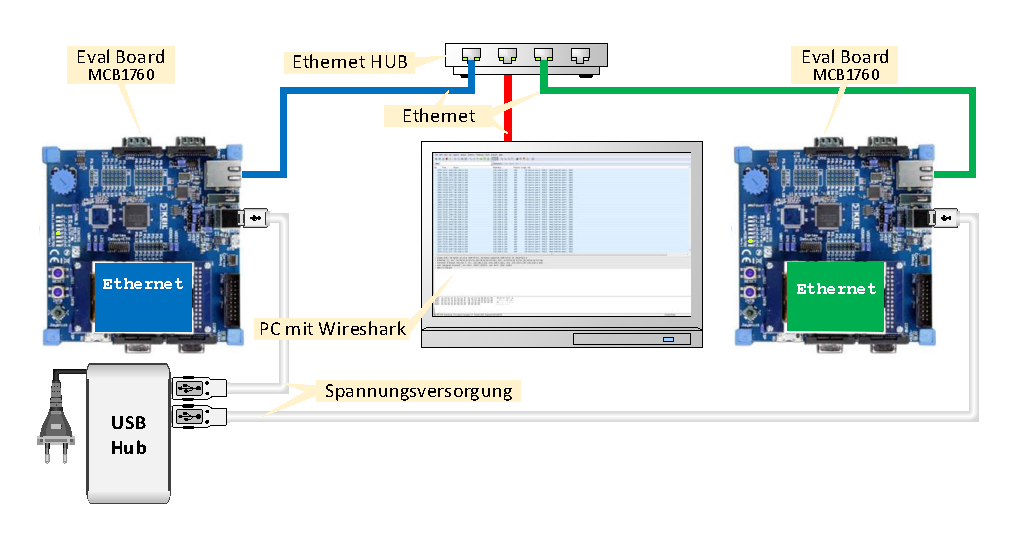
\includegraphics[width=1\textwidth]{images/EthernetAufbau.pdf}
		\caption[Demonstrator Ethernet zwischen zwei Eval Boards]{Demonstrator f�r die Kommunikation zwischen zwei MCB1760 Evaluation Boards �ber Ethernet}
	\label{fig:DemonstratorEthernet}
\end{figure}

Zur Implementierung und Demonstration der Kommunikation �ber Ethernet wurde eine Entwicklungsumgebung entsprechend \autoref{fig:DemonstratorEthernet} aufgebaut. Die beiden Eval Boards sind �ber ein Patchkabel mit einen Hub verbunden. Der Hub hat gegen�ber einem Switch oder Router den Nachteil, dass er eine geringere nutzbare Bandbreite mit sich bringt. Grund daf�r ist, dass der Hub ein Datenpaket immer an jedes angeschlossene Ger�t sendet, unabh�ngig davon, ob das Datenpaket an das Ger�t adressiert wurde oder nicht. Jedoch unterst�tzt dieses Defizit bei der Implementierung, indem mit Hilfe eines PCs und des Tools Wireshark der Datenverkehr zwischen den beiden Eval Boards abgeh�rt wird. Da die versendeten Datenpakete eine Gr��e von zwei Bytes haben, spielt die nutzbare Bandbreite im Rahmen dieser Arbeit keine Rolle. Die in \autoref{fig:DemonstratorEthernet} in wei� eingezeichneten USB-Leitungen dienen zur Spannungsversorgung der Eval Boards.
\pagebreak

\subsection{Anforderungen}\label{subsec:Anforderungen} 

\begin{figure}[b!]
	\centering
		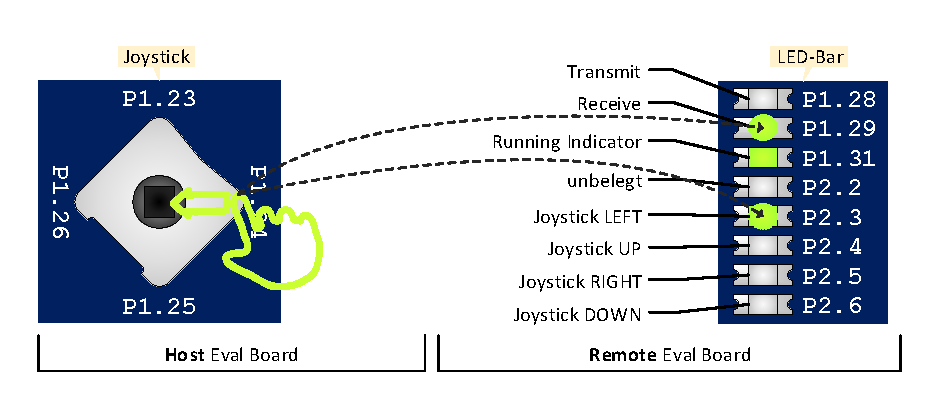
\includegraphics[width=1\textwidth]{images/EthernetSzenario.pdf}
		\caption[Beispiel mit Zuordnung der LEDs]{Beispiel mit Zuordnung der LEDs.}
	\label{fig:EthernetSzenario}
\end{figure}

Zur Demonstration einer funktionsf�higen Ethernet-Kommunikation soll ein exemplarisches Szenario implementiert werden. So sollen LEDs durch den Joystick auf dem jeweils anderen Board ein- und ausgeschaltet werden. Dabei soll die Position des Joysticks angeben, welche LED die LED-Bar ein- oder ausschaltet. Des Weiteren soll das Display die zuletzt empfangene Position anzeigen. Damit die Eval Boards einfach zu identifizieren sind, soll das Display zudem die Host IP Adresse sowie die Remote IP Adresse darstellen. Beim Senden sowie beim Empfangen eines Datenpakets soll der Transmitter bzw. der Receiver kurzzeitig eine LED blinken lassen. Die Zuordnung von Funktionen zu den LEDs der LED-Bar ist \autoref{fig:EthernetSzenario} rechts dargestellt. 

Zudem veranschaulicht \autoref{fig:EthernetSzenario} das Funktionsprinzip. Auf dem Host Eval Board bewegt der Benutzer den Joystick in die linke Richtung. Das f�hrt dazu, dass beim Remote Eval Board die Receiver LED P1.29 kurzzeitig aufleuchtet, sowie die LED P2.3 dauerhaft angeschaltet wird. Bewegt der Benutzer den Joystick erneut in die linke Richtung, erlischt die LED P2.3 wieder.

\subsection{Architektur}\label{subsec:Architektur} 
Bei der Formulierung der Anforderungen in \autoref{subsec:Anforderungen} wurde darauf geachtet, dass diese in m�glichst aktiver Form spezifiziert sind. Dadurch k�nnen die ben�tigten Klassen abgeleitet werden, welches sich im Folgenden durch die �hnlichkeit von Subjekten oder Objekten zu den Klassennamen widerspiegelt.

\begin{figure}[b!]
	\centering
		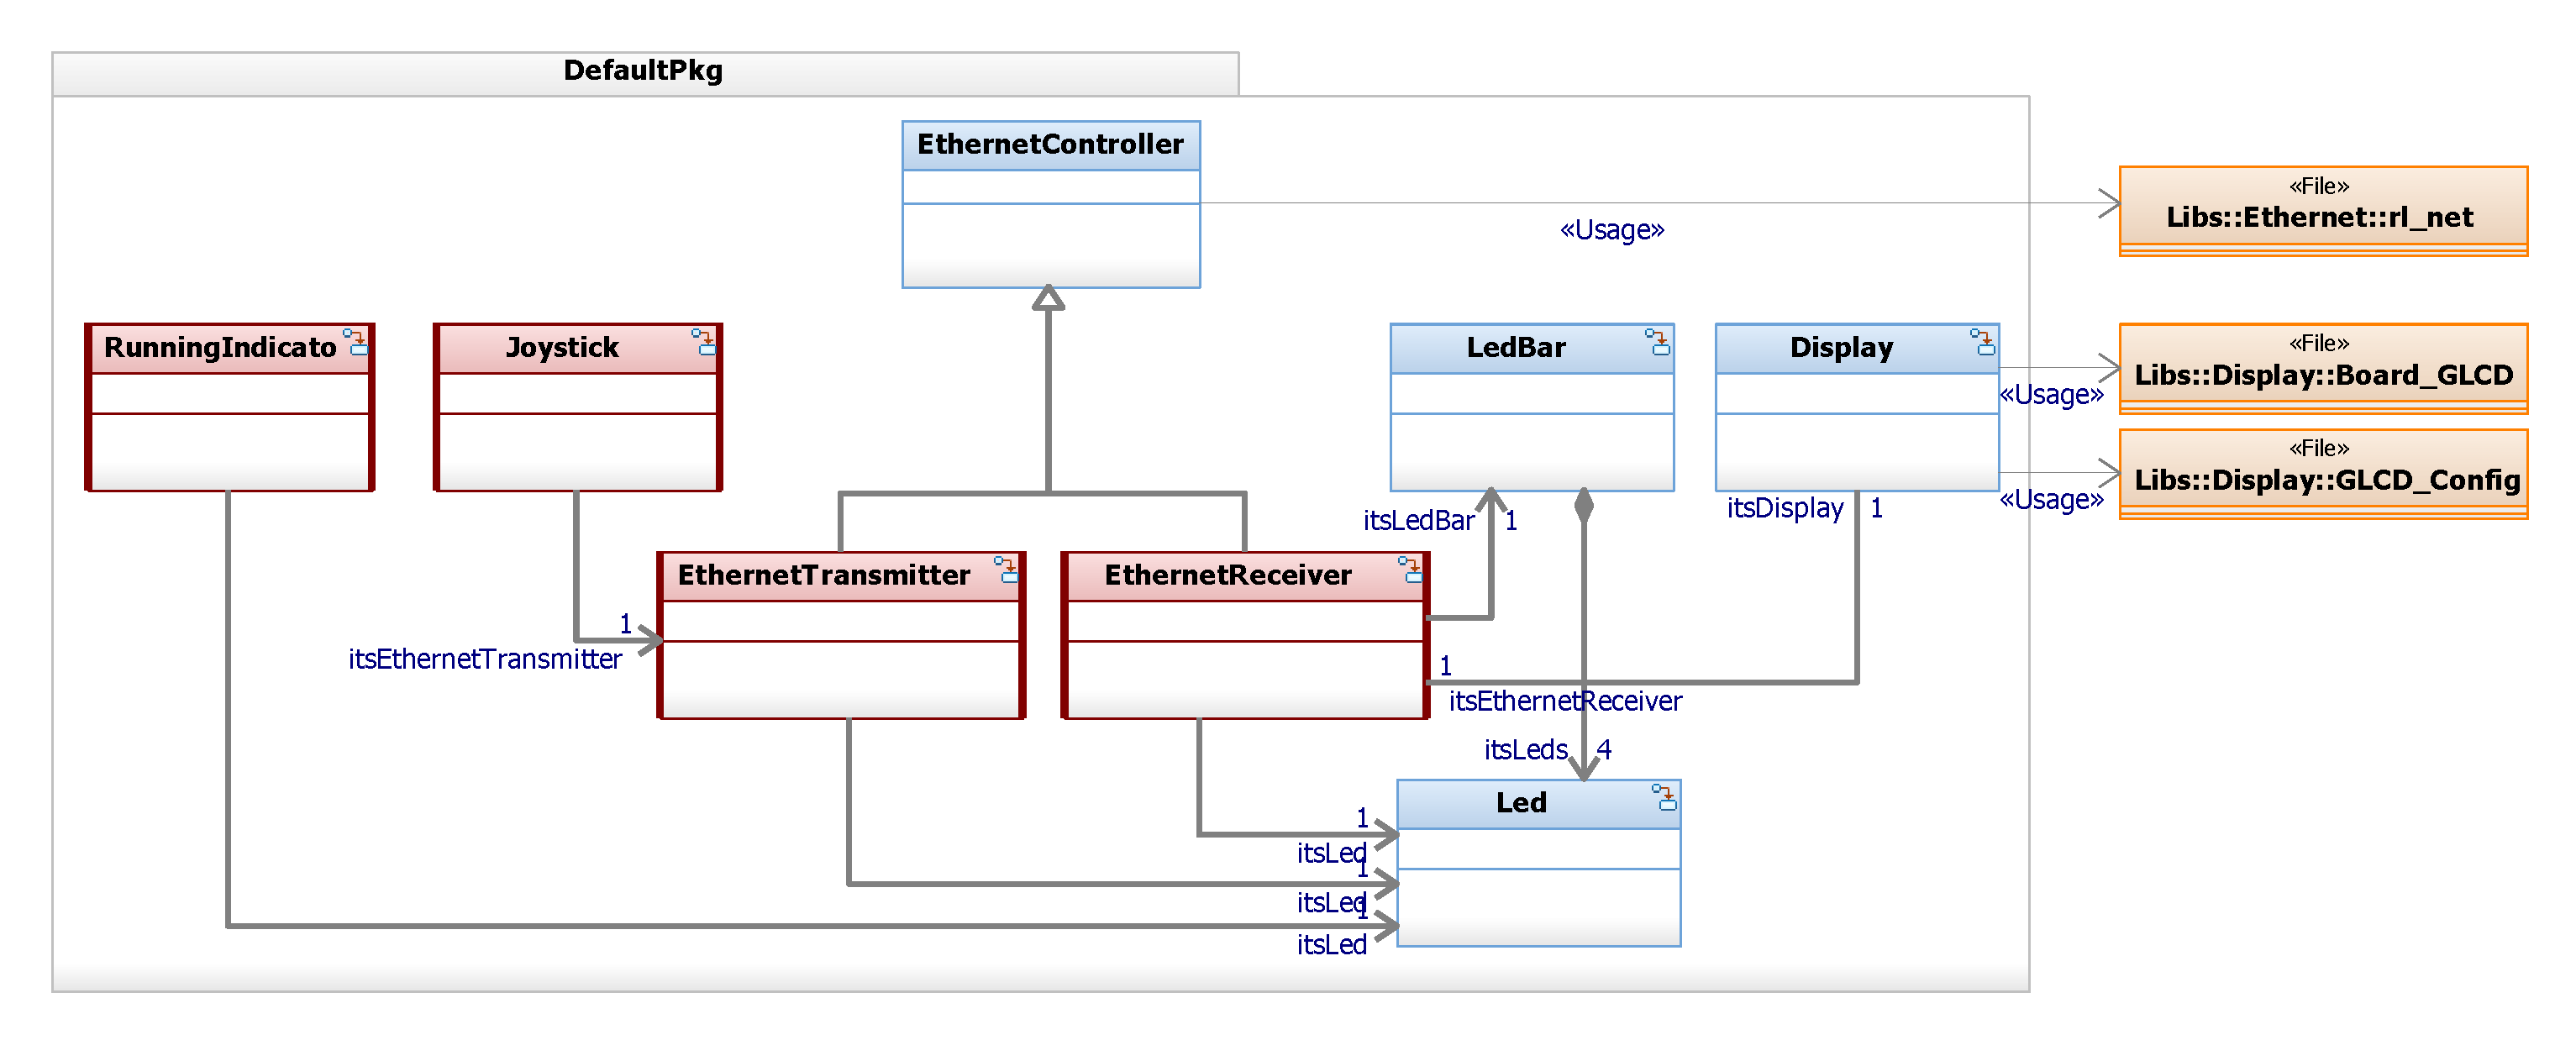
\includegraphics[width=1\textwidth]{images/ClassDiagramEthernet.pdf}
		\caption{Klassendiagramm zur Ethernet-Kommunikation. Klassen, die in eigenen Tasks laufen sind rot eingezeichnet.}
	\label{fig:ClassDiagramEthernet}
\end{figure}

Die Architektur der Ethernet-Kommunikation ist als Klassendiagramm in \autoref{fig:ClassDiagramEthernet} dargestellt. Zentrales Element ist die Basisklasse \texttt{Ether\-net\-Con\-trol\-ler}, von ihr werden die beiden Klassen \texttt{Ether\-net\-Transmitter} und \texttt{Ether\-net\-Receiver} abgeleitet. Diese beiden Klassen arbeiten in separaten Tasks und sind f�r das Senden und Empfangen von Datenpaketen verantwortlich. Auf der linken Seite in \autoref{fig:ClassDiagramEthernet} sind die Klassen \texttt{Running\-Indicator\-Led} und \texttt{Joystick} abgebildet, welche ebenfalls in eigenen Tasks ausgef�hrt werden. Die Klasse \texttt{Running\-Indicator\-Led} l�sst die LED P1.31 zyklisch blinken, mit einer Periodendauer von einer Sekunde. Sie dient zu Debugging zwecken und um unmittelbar zu erkennen, ob das Target l�uft. Die Klasse \texttt{Joystick} pollt regelm��ig die Position des Joysticks. Auf der rechten Seite sind die Klassen \texttt{LedBar}, \texttt{Display} und \texttt{Led} zu finden. Dabei liegt zwischen den Klassen \texttt{LedBar} und \texttt{Led} eine Komposition mit der Multiplizit�t vier vor, wodurch der LED-Bar die LEDs zugeordnet sind, welche eine Joystick Position repr�sentieren. Au�erhalb des Pakets \texttt{DefaultPkg} sind Abh�ngigkeiten zu externen Bibliotheken in orange eingezeichnet. Die verwendeten Bibliotheken, Network und Graphics Component, stammen aus der MDK Middleware und vereinfachen das Verwenden dieser Peripherieger�te. M�gliche Vorgehensweisen beim Einbinden externer Quellen beschreiben \citet{ExternalSources}.

\subsection{Design und Coding}\label{subsec:EthDesignUndCoding} 
In diesem Kapitel werden Attribute, Funktionen und Statecharts wichtiger Klassen im Detail vorgestellt.

\subsubsection*{Ethernet-Controller, Transmitter und Receiver}
Der Ethernet-Controller basiert auf der MDK Middleware Network Component in der Version 7.4.1. Die Network Component beinhaltet eine Vielzahl an Services, Sockets (TCP, UDP und BSD), sowie eine Ethernet Schnittstelle inklusive eines IPv4/IPv6 Protocol Stacks. In dieser Arbeit wird der BSD Socket als Datagram Socket (UDP) zusammen mit dem IPv4 Protocol Stack verwendet. Der BSD Socket stellt eine API zur Verf�gung, die das Aufbauen und Abhandeln einer Netzwerkkommunikation unterst�tzt. Urspr�nglich wurden die BSD Sockets f�r unixnahe Betriebssysteme entwickelt. Mittlerweile sind sie in den POSIX Standard aufgenommen und wurden auch von Microsoft Windows �bernommen. Ein Vorteil der BSD Sockets ist, dass mit geringem Konfigurationsaufwand zwischen Stream Sockets (TCP) und Datagram Sockets (UDP) gewechselt werden kann. 

Die Klasse \texttt{Ether\-net\-Con\-trol\-ler} mit ihren Attributen und Operationen ist in \autoref{fig:EthernetController} dargestellt. Zum Spezifizieren der IP-Adressen dienen die Attribute \texttt{hostIpAddr} und \texttt{remoteIpAddr} vom Typ String. Die IP-Adresse werden in Rhapsody �ber den Features Dialog der beiden Attribute initial festgelegt. Zum Flashen des zweiten Targets k�nnen die IP-Adressen einfach getauscht werden.

\begin{figure}[h!]
	\centering
		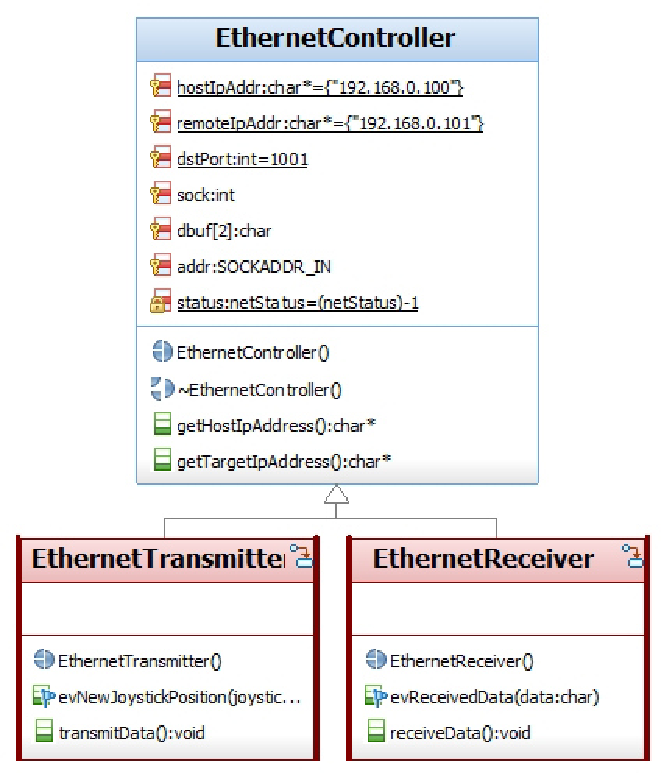
\includegraphics[width=0.49\textwidth]{images/EthernetController.pdf}
		\caption{Basisklasse des Ethernet-Controllers mit abgeleiteten Klassen.}
	\label{fig:EthernetController}
\end{figure}

\paragraph{Initialisierung:}
\autoref{lst:EthernetControllerConstructor} zeigt den Konstruktor des \texttt{Ether\-net\-Con\-trol\-lers}. Der Konstruktor verwendet ausschlie�lich Funktionen der Network Component, was am Prefix \texttt{net} zu erkennen ist. In \autoref{netInitialize} wird die Funktion \texttt{netInitialize} aufgerufen. Diese Funktion muss bei Systemstart einmalig ausgef�hrt werden. Sie initialisiert Systemressourcen, Protokolle und zwei Tasks f�r den Network Core. Bei erfolgreicher Initialisierung wird dem Attribut \texttt{status} der Wert \texttt{netOK} zugewiesen. Mit der �bergeordneten Abfrage wird sichergestellt, dass die Initialisierung auch nur einmalig durchgef�hrt wird, auch wenn der Konstruktor des \texttt{Ether\-net\-Con\-trol\-lers} durch die beiden Instanzen der abgeleiteten Klassen zweimal durchlaufen wird. Die Funktion \texttt{netIP\_aton} konvertiert eine IP-Adresse vom Typ String in eine bin�re Form. Dadurch ist es anschlie�end m�glich, die Host IP-Adresse dynamisch mit Hilfe der Funktion \texttt{netIF\_SetOption} zu setzen. Somit ist die Konfiguration der Host IP-Adresse ebenfalls in Rhapsody m�glich und ben�tigt keine manuelle Anpassung innerhalb der Keil Umgebung.

\lstset{escapechar=@, escapeinside={(*@}{@*)}, style=customcpp}
\begin{lstlisting}[caption={Konstruktor des Ethernet-Controllers}, label={lst:EthernetControllerConstructor}, captionpos=b]
unsigned char buf[8];

if (status != netOK)   
{	
	// Initialize the network component only once
	status = netInitialize (); (*@\label{netInitialize}@*)

	// Set the host ip address once
	netIP_aton (hostIpAddr, NET_ADDR_IP4, buf);
	netIF_SetOption (
		NET_IF_CLASS_ETH | 0, 
		netIF_OptionIP4_Address, 
		buf, 
		NET_ADDR_IP4_LEN);
}
\end{lstlisting}

\begin{figure}
	\centering
	\subfigure[Initialisierung und Sendeablauf des Ethernet-Transmitters.]{
					\label{fig:EthernetTransmitter}
					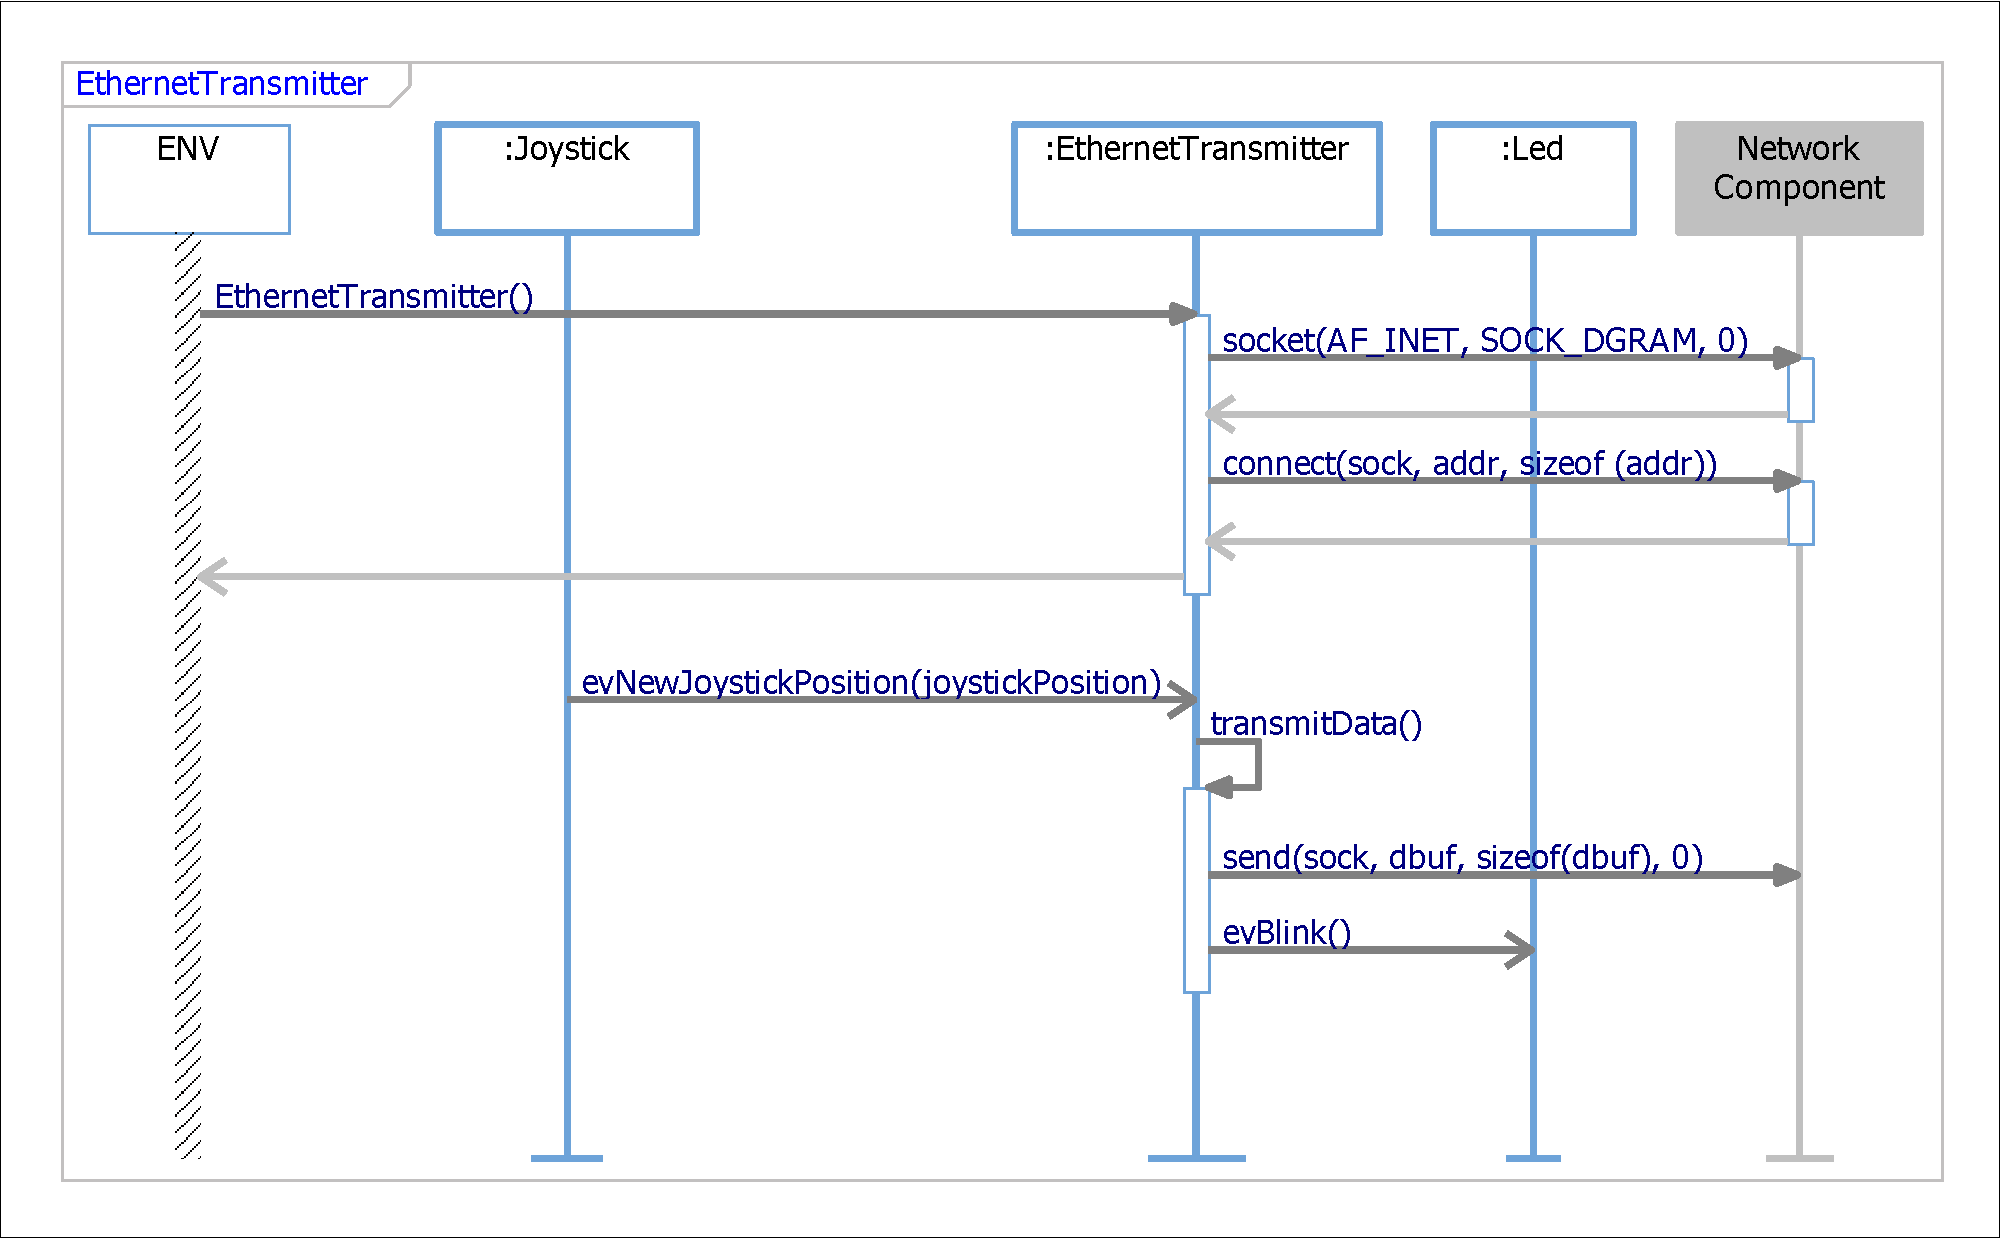
\includegraphics[width=1\textwidth]{images/EthernetTransmitter.pdf}
	}
	\subfigure[Initialisierung des Ethernet-Receivers und Ablauf beim Empfangen von Daten.]{
					\label{fig:EthernetReceiver}
					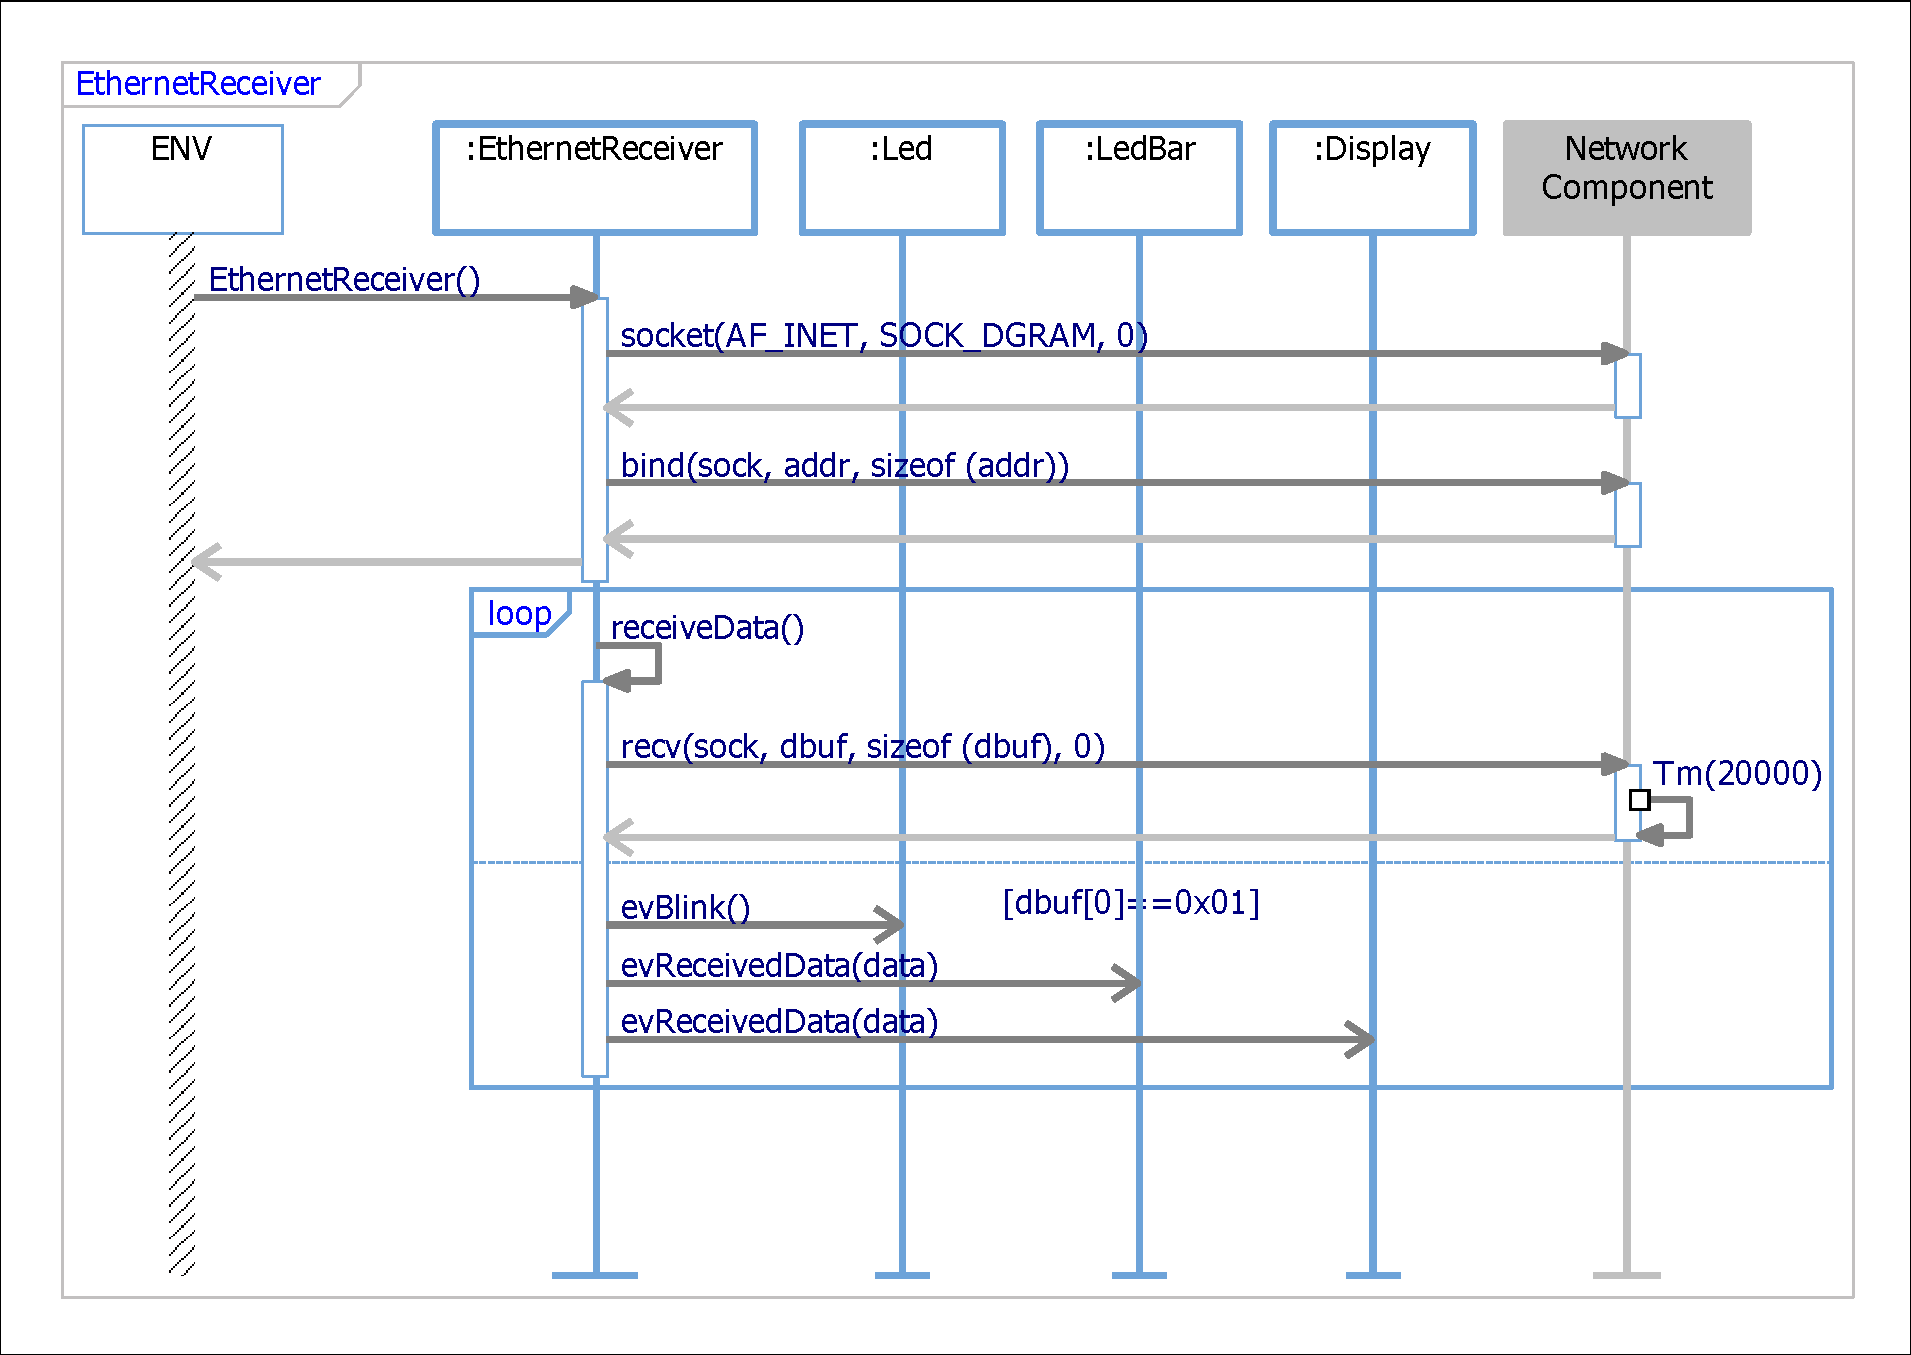
\includegraphics[width=1\textwidth]{images/EthernetReceiver.pdf}
	}
	\caption{Sequenzdiagramme des Ethernet-Transmitters und -Receivers.}
	\label{fig:EthernetTransCeiver}
\end{figure}

\paragraph{Daten senden:}
Das Sequenzdiagramm in \autoref{fig:EthernetTransmitter} stellt das Verhalten des Ethernet-Transmitters dar. Der \texttt{Ether\-net\-Transmitter} erstellt in seinem Konstruktor einen Socket vom Typ Datagram Sockets (UDP), zu erkennen am �bergabeparameter \texttt{SOCK\_DGRAM}. Dem Socket wei�t er durch Aufruf von \texttt{connect} die Remote IP-Adresse, also die IP-Adresse des anderen Endpunkts, zu. Aufgrund des gew�hlten Typ Datagram Sockets (UDP), richtet der \texttt{Ether\-net\-Transmitter} zudem ein Adressfilter zwischen den Endpunkten ein. Im weiteren Ablauf befindet sich der Ethernet-Transmitter im Grunde im Leerlauf und wartet auf das Event \texttt{evNew\-Joy\-stick\-Position} welches vom Joystick abgefeuert wird. Trifft das Event \texttt{evNew\-Joy\-stick\-Position} ein, handelt der \texttt{Ether\-net\-Transmitter} durch die Operation \texttt{tran\-smit\-Data} seine Sendeaktivit�ten ab. Die Funktion \texttt{send} sorgt daf�r, dass die Daten im Buffer \texttt{dbuf} �bertragen werden. Zum Abschluss sendet die Klasse \texttt{Ether\-net\-Transmitter} das Event \texttt{evBlink} an die zugeh�rige LED, was dazu f�hrt, dass die Sende-LED P1.28 einmalig blinkt. 

\paragraph{Daten empfangen:}
Der \texttt{Ether\-net\-Receiver} erstellt in seinem Konstruktor ebenfalls einen Socket vom Typ Datagram Sockets (UDP) und bindet diesen mit der Funktion \texttt{bind} an die Remote IP-Adresse sowie an den Ziel-Port. Der Ziel-Port \texttt{dstPort} kann f�r beide Targets gleich bleiben, er definiert an welchem Port auf eingehende Datenpakete gehorcht wird. Anschlie�end durchl�uft der \texttt{Ether\-net\-Transmitter} eine Endlosschleife. In dieser ruft er seine Operation \texttt{receiveData} auf, welche das Empfangen von Daten behandelt. Die Funktion \texttt{recv} empf�ngt eingehende Daten auf dem zuvor spezifizierten Port. Wenn der Network Core erkennt, dass ein Betriebssystem im Einsatz ist, betreibt der Network Core die Funktion \texttt(recv) automatisch im Blocking Mode. Dadurch ist es zwingend erforderlich, dass die Klasse \texttt{Ether\-net\-Receiver} in einem separaten Task ausgef�hrt wird. Der Blocking Mode ist zudem mit einem Timeout verbunden, der bei Ablauf in den Errorcode \texttt{BSD\_ERROR\_TIMEOUT} resultiert. Nach Ablauf der vorkonfigurierten Zeit von 20 Sekunden, oder falls zuvor Daten Empfangen wurden, ruft der \texttt{Ether\-net\-Receiver} die Funktion \texttt{recv} erneut auf. Hat der \texttt{Ether\-net\-Receiver} Daten Empfangen, werden diese auf ihre G�ltigkeit �berpr�ft. Dazu dient ein minimales Protokoll, dessen erstes Byte zur Synchronisation dient. Sind keine g�ltigen Daten vorhanden, endet die Operation \texttt{receiveData} an dieser Stelle. Entspricht das erste Byte dem Synchronisations-Byte 0x01, feuert der \texttt{Ether\-net\-Receiver} das Event \texttt{evBlink} an seine LED, damit die Empfangs-LED P1.29 blinkt. Zudem sendet er das Event \texttt{evReceivedData} mit dem Inhalt des zweiten Bytes an die LED-Bar, sowie an das Display. Auf der LED-Bar wird das Datenbyte ausgewertet und die entsprechende LED ein- oder ausgeschaltet. Das Verhalten des \texttt{Ether\-net\-Receiver} ist in \autoref{fig:EthernetReceiver} dargestellt.

Somit gibt es je Target einen \texttt{Ether\-net\-Transmitter} und einen \texttt{Ether\-net\-Re\-cei\-ver}, die in eigenen Tasks ihre Routinen durchlaufen. 

\subsubsection*{Joystick}

Der Joystick verf�gt in Summe �ber sechs verschiedene Richtungen, von denen die vier Richtungen links, rechts, oben und unten von Interesse sind. Das Abtasten und Auslesen der Position des Joysticks erfolgte in Anlehnung an \citet{Schwerin17}. Dabei wurde die Auswertung der Joystick Position um ein Filter erg�nzt, damit nur relevante und neue Positionen via Ethernet �bertragen werden. Ursache daf�r ist, dass der Joystick nach der Bet�tigung, in eine der zuvor aufgez�hlten Richtung, wieder in die zentrale Position zur�ckkehrt. Dadurch nimmt der Joystick eine f�r ihn neue Position ein und w�rde ohne Filter das Senden eines Datenpakets triggern. \autoref{lst:JoystickFilter} zeigt die Implementierung des Filters. Bewegt sich der Joystick in die mittige Position, wird nie ein Event abgefeuert. Hat der Joystick eine andere Richtung eingenommen, feuert die Klasse \texttt{Joystick} das Event \texttt{evNewJoy\-stick\-Position} an den \texttt{Ether\-net\-Transmitter}.

Die Klasse \texttt{Joystick} h�lt die Position f�r eine Dauer von 100 Millisekunden, liest im Anschluss daran den aktuellen Wert aus dem entsprechenden Register aus und filtert diesen. Dieses Sample-and-Hold-Verhalten wurde im zugeh�rigen Statechart modelliert. Die Halte-Dauer kann im Konstruktor der Klasse \texttt{Joystick} angepasst werden.

\lstset{escapechar=@, escapeinside={(*@}{@*)}, style=customcpp}
\begin{lstlisting}[caption={Filter zur Auswertung der Joystick Position}, captionpos=b, label={lst:JoystickFilter}]
int position = (LPC_GPIO1->FIOPIN >> 20) & Joystick_Mask;

// Bit 4-7 contain the position information
position = position >> 3; (*@\label{joystickPosition}@*)

if (position == Joystick_CENTER)
{   
	// If the Joystick got back to center only update
	lastPosition = position;  
}
else if (position != lastPosition)
{
	lastPosition = position;    	
	FIRE( this->itsEthernetTransmitter, evNewJoystickPosition(position)); 
}   
\end{lstlisting}

\subsubsection*{LED-Bar und Display}

Die LED-Bar und das Display sind die Empf�nger des Events \texttt{evReceivedData}, welches der Ethernet-Receiver mit dem Inhalt des Datenbytes als Parameter abfeuert. Die Klasse \texttt{LedBar} ordnet den empfangenen Parameter der entsprechenden LED zu und ruft die Operation \texttt{toggleLed} der Klasse \texttt{Led} auf. Die Klasse \texttt{Display} nutzt ebenfalls den empfangenen Parameter und zeigt damit die zuletzt empfangene Richtung an. Wie in \autoref{fig:EthernetDisplay} dargestellt, zeigt das Display zudem die Host und die Remote IP-Adresse an.

\begin{figure}[h!]
	\centering
	\subfigure[Blauer Hintergrund bei Host IP 192.168.0.101.]{
					\label{fig:EthernetDisplay1}
					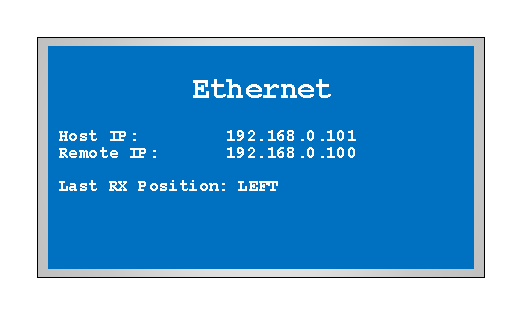
\includegraphics[width=0.45\textwidth]{images/EthernetDisplay1.pdf}
	}
	\subfigure[Gr�ner Hintergrund bei Host IP 192.168.0.100.]{
					\label{fig:EthernetDisplay2}
					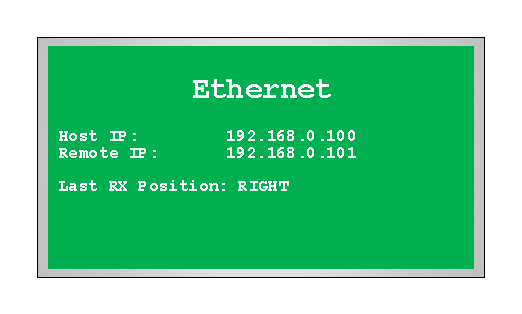
\includegraphics[width=0.45\textwidth]{images/EthernetDisplay2.pdf}
	}
	\caption{Beispielhafte Ausgaben auf dem Display f�r die Ethernet Applikation.}
	\label{fig:EthernetDisplay}
\end{figure}

\subsection{Konfigurieren des Keil Projekts}

Als Basis f�r die Implementierung wurde das Blinky-Beispielprojekt verwendet, welches im RXF \textit{Rpy\_CPP\_CMSIS\_Keil5\_ARM\_MCB1700\_TD} von Willert enthalten ist. Zwar ist das Keil Projekt lediglich rudiment�r konfiguriert, stellt aber die funktionsf�hige Einbindung von Rhapsody sicher. Im Folgenden werden die wichtigsten Anpassungen in der Konfiguration gegen�bergestellt.

\subsubsection*{Manage Run-Time Environment} 

Mittels des Konfigurationsassistenten 
\includegraphics[width=0.3cm]{images/package.pdf} \textit{Manage Run"=Time Environment} ist es m�glich, Software Komponenten einem Keil Projekt hinzuzuf�gen. Mit dem Ziel eine Ethernet Kommunikation aufzubauen, wird zun�chst der Software Pack \textit{Keil::MDK"=Middleware} in der Version 7.4.1 (2017-04-21) dem Projekt hinzugef�gt. Diese Paket beinhaltet unter anderem die Network Component in der Version 7.5.0 (2017-04-21). Zum Betreiben der Network Component wird der \textit{ARM::CMSIS:CORE} in der Version 5.0.1 vorausgesetzt. Die dazu notwendige �nderung im Ethernet Projekt gegen�ber dem Blinky Projekt ist in \autoref{tab:RuntimeEnv} rot gekennzeichnet.

Die Network Component beinhaltet eine Vielzahl an Komponenten, die dem Keil Projekt hinzugef�gt werden k�nnen. F�r den vorliegenden Fall der Ethernet"=Kommunikation sind die Komponenten und die ben�tigten CMSIS Treiber gem�� \autoref{tab:RuntimeEnv} zu w�hlen. Notwendige Anpassungen zur Verwendung des Displays sind orange markiert.

\begin{table}[!ht]
\centering
\footnotesize
\begin{tabular}{p{0.01mm}p{4.6cm}p{0.2cm}p{2.2cm}lp{0.2cm}p{2.2cm}l}
	\toprule
	& & \multicolumn{3}{ c }{Blinky} & \multicolumn{3}{ c }{Ethernet} \\ \cmidrule{3-5}  \cmidrule{6-8}
	& Software Component & Sel. & Variant & Version & Sel. & Variant & Version \\
	\midrule
	& $\boxminus$\textSFx 
\includegraphics[width=0.25cm]{images/package.pdf} Board Support & & \tiny{MCB1700} & & \cellcolor{KeilGreen} & \tiny{MCB1700} & \\
	& \textSFxi\hspace{2ex}$\boxminus$\textSFx 
\includegraphics[width=0.25cm]{images/package.pdf} Graphic LCD (API) &  &  & 1.0.0 & \cellcolor{KeilGreen} &  & 1.0.0 \\
	\textcolor{Orange}{ \pmboxdrawuni{258E}} & \textSFxi\hspace{2ex}\textSFii\textSFx\textSFx	
\includegraphics[width=0.2cm]{images/item.pdf} Graphic LCD & \HollowBox &  & 1.0.0 & \cellcolor{KeilGreen}\CheckedBox &  & 5.0.1 \\
	& $\boxminus$\textSFx 
\includegraphics[width=0.25cm]{images/package.pdf} CMSIS & \cellcolor{KeilGreen} & & & \cellcolor{KeilGreen} & & \\
	\textcolor{Red}{ \pmboxdrawuni{258E}} & \textSFxi\hspace{2ex}\textSFii\textSFx\textSFx	
\includegraphics[width=0.2cm]{images/item.pdf} CORE & \cellcolor{KeilGreen}\CheckedBox  &  & 4.3.0 & \cellcolor{KeilGreen}\CheckedBox &  & 5.0.1 \\
	& $\boxminus$\textSFx 
\includegraphics[width=0.25cm]{images/package.pdf} CMSIS Driver & & & & \cellcolor{KeilGreen} & & \\
	& \textSFxi\hspace{2ex}$\boxminus$\textSFx 
\includegraphics[width=0.25cm]{images/package.pdf} Ethernet MAC (API) & & & 2.01 & \cellcolor{KeilGreen} &  & 2.1.0 \\
	\textcolor{Yellow}{ \pmboxdrawuni{258E}} & \textSFxi\hspace{2ex}\textSFxi\hspace{2ex}\textSFii\textSFx\textSFx 
\includegraphics[width=0.20cm]{images/item.pdf} Ethernet MAC & \HollowBox  &  & 2.9 & \cellcolor{KeilGreen}\CheckedBox &  & 2.9.0 \\
	& \textSFxi\hspace{2ex}$\boxminus$\textSFx 
\includegraphics[width=0.25cm]{images/package.pdf} Ethernet PHY (API) & & & 2.00 & \cellcolor{KeilGreen} &  & 2.1.0 \\
	\textcolor{Yellow}{ \pmboxdrawuni{258E}} & \textSFxi\hspace{2ex}\textSFxi\hspace{2ex}\textSFii\textSFx\textSFx 
\includegraphics[width=0.20cm]{images/item.pdf} DP83848C & \HollowBox  &  & 6.1 & \cellcolor{KeilGreen}\CheckedBox &  & 6.1.0 \\
	& \textSFxi\hspace{2ex}$\boxminus$\textSFx 
\includegraphics[width=0.25cm]{images/package.pdf} SPI (API) & & & 2.01 & \cellcolor{KeilGreen} &  & 2.2.0 \\
	& \textSFxi\hspace{5ex}\textSFviii\textSFx\textSFx 
\includegraphics[width=0.20cm]{images/item.pdf} SPI & \HollowBox  &  & 2.1 & \HollowBox &  & 2.1.0 \\
	\textcolor{Orange}{ \pmboxdrawuni{258E}} & \textSFxi\hspace{5ex}\textSFii\textSFx\textSFx 
\includegraphics[width=0.20cm]{images/item.pdf} SSP & \HollowBox  &  & 2.5 & \cellcolor{KeilGreen}\CheckedBox &  & 2.7.0 \\
	& $\boxminus$\textSFx 
\includegraphics[width=0.25cm]{images/package.pdf} Device & & & & \cellcolor{KeilGreen} & & \\
	\textcolor{Orange}{ \pmboxdrawuni{258E}}
 & \textSFxi\hspace{2ex}\textSFviii\textSFx\textSFx 
\includegraphics[width=0.20cm]{images/item.pdf} GPDMA & \HollowBox &  & 1.2 & \cellcolor{KeilGreen}\CheckedBox &  & 1.2.0 \\
	\textcolor{Yellow}{ \pmboxdrawuni{258E}} & \textSFxi\hspace{2ex}\textSFviii\textSFx\textSFx 
\includegraphics[width=0.20cm]{images/item.pdf} GPIO & \HollowBox &  & 1.1 & \cellcolor{KeilGreen}\CheckedBox &  & 1.1.0 \\
	\textcolor{Yellow}{ \pmboxdrawuni{258E}} & \textSFxi\hspace{2ex}\textSFviii\textSFx\textSFx 
\includegraphics[width=0.20cm]{images/item.pdf} PIN & \HollowBox &  & 1.0 & \cellcolor{KeilGreen}\CheckedBox &  & 1.0.0 \\
	& \textSFxi\hspace{2ex}\textSFii\textSFx\textSFx 
\includegraphics[width=0.20cm]{images/item.pdf} Startup & \cellcolor{KeilGreen}\CheckedBox &  & 1.0.0 & \cellcolor{KeilGreen}\CheckedBox &  & 1.0.0 \\
	& $\boxminus$\textSFx 
\includegraphics[width=0.25cm]{images/package.pdf} Network & & \tiny{MDK-Pro} & 7.4.0 & \cellcolor{KeilGreen} & \tiny{MDK-Pro} & 7.5.0 \\
	\textcolor{Yellow}{ \pmboxdrawuni{258E}} & \hspace{3.2ex}\textSFviii\textSFx\textSFx 
\includegraphics[width=0.20cm]{images/item.pdf} CORE & \HollowBox & \tiny{IPv4/IPv6 Release} & 7.4.0 & \cellcolor{KeilGreen}\CheckedBox & \tiny{IPv4/IPv6 Release} & 7.5.0 \\
	& \hspace{3.2ex}\textSFviii\textSFx\textSFx 
\includegraphics[width=0.20cm]{images/item.pdf} Legacy API & \HollowBox &  & 7.4.0 & \HollowBox &  & 7.5.0 \\
	& \hspace{3.2ex}$\boxminus$\textSFx 
\includegraphics[width=0.25cm]{images/package.pdf} Interface & & & & \cellcolor{KeilGreen} &  & \\
	\textcolor{Yellow}{ \pmboxdrawuni{258E}} & \hspace{3.2ex}\textSFxi\hspace{2ex}\textSFviii\textSFx\textSFx 
\includegraphics[width=0.20cm]{images/items.pdf} ETH & 0  &  & 7.4.0 & \cellcolor{KeilGreen} 1 &  & 7.5.0 \\
	& \hspace{3.2ex}\textSFxi\hspace{2ex}\textSFviii\textSFx\textSFx 
\includegraphics[width=0.20cm]{images/item.pdf} PPP & \HollowBox &  & 7.4.0 & \HollowBox &  & 7.5.0 \\
	& \hspace{3.2ex}\textSFxi\hspace{2ex}\textSFii\textSFx\textSFx 
\includegraphics[width=0.20cm]{images/item.pdf} SLIP & \HollowBox &  & 7.4.0 & \HollowBox &  & 7.5.0 \\
	& \hspace{3.2ex}$\boxplus$\textSFx
\includegraphics[width=0.25cm]{images/package.pdf} Service & & & & & & \\
	& \hspace{3.2ex}$\boxminus$\textSFx
\includegraphics[width=0.25cm]{images/package.pdf} Socket & & & & \cellcolor{KeilGreen} & & \\
	\textcolor{Yellow}{ \pmboxdrawuni{258E}} & \hspace{6.3ex}\textSFviii\textSFx\textSFx 
\includegraphics[width=0.20cm]{images/item.pdf} BSD & \HollowBox &  & 7.4.0 & \cellcolor{KeilGreen}\CheckedBox &  & 7.5.0 \\
	\textcolor{Yellow}{ \pmboxdrawuni{258E}} & \hspace{6.3ex}\textSFviii\textSFx\textSFx 
\includegraphics[width=0.20cm]{images/item.pdf} TCP & \HollowBox &  & 7.4.0 & \cellcolor{KeilGreen}\CheckedBox &  & 7.5.0 \\
	\textcolor{Yellow}{ \pmboxdrawuni{258E}} & \hspace{6.3ex}\textSFii\textSFx\textSFx 
\includegraphics[width=0.20cm]{images/item.pdf} UDP & \HollowBox &  & 7.4.0 & \cellcolor{KeilGreen}\CheckedBox &  & 7.5.0 \\
	\bottomrule
\end{tabular}
\caption{Heraufsetzen des CMSIS:CORE (rot), ben�tigte Komponenten der Network Component und deren Abh�ngigkeiten (gelb), sowie die Komponenten zum Betreiben des Displays (orange).}
\label{tab:RuntimeEnv}
\end{table}

\subsubsection*{Target Options}

Mit der Aufnahme der Network Component in das Keil Projekt, steigt der erforderliche RAM-Speicherbedarf der Applikation auf �ber 41KB (RW-data=352 Bytes + ZI-data=41176 Bytes). Damit wird die vorkonfigurierte RAM-Speichergr��e von 32KB �berschritten. Jedoch verf�gt das Keil MCB1760 Evaluation Board �ber insgesamt 64KB RAM On-Chip Memory, so dass die weiteren 32KB RAM mit Hilfe des Scatter Files adressiert werden m�ssen. Das Scatter File (.sct) befindet sich im Flash-Ordner des Keil-Projekts. Allerdings bietet Keil die M�glichkeit, dass Scatter File �ber die Bedienoberfl�che zu generieren, so dass das Scatter File nicht direkt editiert werden muss. �ber die \begin{itshape}Target Options\end{itshape} im Reiter \begin{itshape}Target\end{itshape} k�nnen im Panel \begin{itshape}Read/Write Memory Areas\end{itshape} die zweiten 32KB RAM-Speicher aktiviert werden. Die Startadresse der zweiten Speicherbank ist mit 0x2007C000 anzugeben, die Gr��e des Speichers von 32KB ebenfalls als hexadezimaler Wert mit 0x8000.

\subsubsection*{CMSIS Configuration}

Bei der CMSIS Configuration geht es prim�r um das Konfigurieren des CMSIS RTX Kernel. Dabei wird die Datei \textit{RTX\_Conf\_CM.c}, die Teil der CMSIS Component ist, editiert. Keil bietet den Komfort, die Datei �ber den integrierten \begin{itshape}Configuration Wizard\end{itshape} zu bearbeiten. Der erste Parameter \textit{Number of concurrent running user threads} im Abschnitt \textit{Thread Configuration} gibt die Anzahl der Tasks an, die zur gleichen Zeit laufen. Die Tasks mit der Ursache CMSIS-RTOS in Tabelle \autoref{tab:DefaultThreads} sind bei jeder Applikation standardm��ig aktiv, die das CMSIS-RTOS verwenden.

\begin{table}[!b]
\centering
\footnotesize
	\begin{tabular}{lcl}
	\toprule
	Task Name & Priorit�t & Ursache \\
	\midrule
	osTimerThread & 1 & CMSIS-RTOS \\
	main & 2 & CMSIS-RTOS \\
	os\_idle\_demon & 255 & CMSIS-RTOS \\
	WST\_\-Monitor\_receiveTask & 3 & Willert RXF \\
	netCore\_Thread & 4 & Network Component \\
	netETH\_Thread & 5 & Network Component \\
	RunningIndicator & 6 & Ethernet Applikation \\
	EthernetReceiver & 7 & Ethernet Applikation \\
	EthernetTransmitter & 8 & Ethernet Applikation \\
	Joystick & 9 & Ethernet Applikation \\
	\bottomrule
	\end{tabular}
\caption{Verwendete Task f�r die Ethernet-Kommunikation und deren Ursache.}
\label{tab:DefaultThreads}
\end{table}

Das Willert RXF bringt durch sein kleines Onboard-Betriebssystem mit \textit{WST\_""Monitor\_""receiveTask} einen weiteren Task mit sich. Zudem beansprucht die Network Component bei der Initialisierung die beiden Tasks \textit{netCore\_Thread} und \begin{itshape}netETH\_Thread\end{itshape}. Zus�tzlich kommen noch die Tasks hinzu, die durch die Applikation an sich gefordert sind. Gem�� der in rot gekennzeichneten Klassen in \autoref{fig:ClassDiagramEthernet} sind das die Tasks \textit{RunningIndicator}, \textit{EthernetReceiver}, \textit{EthernetTransmitter} und \textit{Joystick}. In Summe ergeben sich somit zehn Tasks. Da nach \citet{CmsisRtos2017} der Task \textit{os\_idle\_demon} nicht in die Anzahl der gleichzeitig laufenden Tasks mit eingeht, wird der Parameter \textit{Number of concurrent running user threads} auf den Wert neun gesetzt. 

Unter den weiteren Parametern im Abschnitt \textit{Thread Configuration} ist vor allem der Parameter \textit{Total stack size [bytes] for threads with user-provided stack size} von Interesse.  Dieser muss im Vergleich zum Blinky Projekt um 1024 Bytes f�r den Task \textit{netCore\_Thread} erh�ht werden, sowie um weitere 512 Bytes f�r den Task \textit{netEth\_Thread} \parencite{NetworkComponent2017}. Die Anpassungen f�r die Ethernet"=Kommunikation in der Datei \textit{RTX\_Conf\_CM.c} gegen�ber dem Blinky Projekt sind in \autoref{tab:RtxConfig} aufgelistet.

\begin{table}[!ht]
\footnotesize
\centering
	\begin{tabular}{p{7.6cm}p{3.0cm}p{3.0cm}}
	\toprule
	& Blinky & Ethernet \\ \cmidrule{2-3}
	Option & Value & Value \\
	\midrule
	$\boxminus$\textSFx Thread Configuration & &  \\
	\textSFxi\hspace{2ex}\textSFviii\textSFx\textSFx Number of concurrent running user threads & 6 & 9 (+3) \\
	\textSFxi\hspace{2ex}\textSFviii\textSFx\textSFx Default Thread stack size [bytes] & 200 & 200 \\
	\textSFxi\hspace{2ex}\textSFviii\textSFx\textSFx Main Thread stack size [bytes] & 1024 & 1024 \\
	\textSFxi\hspace{2ex}\textSFviii\textSFx\textSFx Number of threads with user-provided & 5 & 5 \\
	\textSFxi\hspace{2ex}\textSFxi \hspace{1.5ex} stack size &  & \\
	\textSFxi\hspace{2ex}\textSFviii\textSFx\textSFx Total stack size [bytes] for threads with & 4096 & 5632 (+1536)\\
	\textSFxi\hspace{2ex}\textSFxi \hspace{1.5ex} user-provided stack size &  & \\
	\textSFxi\hspace{2ex}\textSFviii\textSFx\textSFx  Check for stack overflow & \CheckedBox &  \CheckedBox \\
	\textSFxi\hspace{2ex}\textSFii\textSFx\textSFx  Processor mode for thread execution & Privileged mode & Privileged mode \\
	$\boxplus$\textSFx RTX Kernel Timer Tick Configuration & & \\
	$\boxplus$\textSFx System Configuration & & \\
	\bottomrule
	\end{tabular}
\caption{Anpassungen in der RTX Configuration \textit{RTX\_Conf\_CM.c}.}
\label{tab:RtxConfig}
\end{table}

\subsubsection*{Device Configuration}

Die Datei \textit{startup\_LPC17xx.s (Startup)} bildet zusammen mit der Datei\linebreak \textit{startup\_LPC17xx.c (Startup)} den Start-up Code, welcher direkt nach einem RESET des Targets ausgef�hrt wird. Die beiden Dateien sind Teil der Device Component und k�nnen ebenfalls �ber den \textit{Configuration Wizard} bearbeitet werden. Von gr��erem Interesse ist die Datei \textit{startup\_LPC17xx.s (Startup)} bei die Zuordnung von Speicher erfolgt. In der Datei \textit{startup\_LPC17xx.c (Startup)} geht es im Wesentlichen um die Clock Konfiguration, welche aber bei ihrer Standardeinstellung belassen wird.

\begin{table}[!b]
\footnotesize
\centering
	\begin{tabular}{p{7.6cm}p{3.0cm}p{3.0cm}}
	\toprule
	& Blinky & Ethernet \\ \cmidrule{2-3}
	Option & Value & Value \\
	\midrule
	$\boxminus$\textSFx Stack Configuration & &  \\
	\textSFxi\hspace{2ex}\textSFii\textSFx\textSFx Stack Size (in Bytes) & 0x0000 0200 & 0x0000 0400 (+512) \\
	$\boxminus$\textSFx Heap Configuration & & \\
  \hspace{3ex}\textSFii\textSFx\textSFx Heap Size (in Bytes) & 0x0000 1000 & 0x0000 1000 \\
	\bottomrule
	\end{tabular}
\caption{Anpassungen in der Startup Configuration \textit{startup\_LPC17xx.s (Startup)} f�r die Ethernet-Kommunikation.}
\label{tab:StartupConfig}
\end{table}

Nach \citet{NetworkComponent2017} ist bei Verwendung des Ethernet Cores eine Verg��erung der Stack Size um 512 Bytes erforderlich. Eine Anpassung des Heaps ist nicht erforderlich, da in dieser Implementierung die Security Komponente nicht verwendet wird. Die �nderung im Startup File ist in \autoref{tab:StartupConfig} dargestellt.

\subsubsection*{Ethernet Network Configuration}

Die Ethernet-Konfiguration erfolgt �ber die Konfigurationsdateien, die zur Network Component geh�ren. Dabei ist in Konfigurationsdatei \textit{Net\_Config\_ETH\_0.h (Interface:ETH)} eine Anpassung vorzunehmen, welche die Option \textit{Dynamic Host Configuration} betrifft. Wenn diese Option aktiviert ist, werden IP-Adresse, Netzmaske und Standardgateway automatisch von einem DHCP Server bezogen. Da der Demonstrationsaufbau �ber keinen DHCP Server verf�gt und die IP-Adressen statisch vergeben werden, muss diese Option deaktiviert werden. \autoref{tab:EthernetNetworkConfig} zeigt, dass die IP-Adresse in dieser Datei auch manuell konfiguriert werden kann. Jedoch wird diese Option zur Laufzeit �berschrieben, da die Implementierungen beschrieben in \autoref{subsec:EthDesignUndCoding} die IP-Adresse festlegen.
 
\begin{table}[!ht]
\footnotesize
\centering
	\begin{tabular}{p{7.6cm}p{3.0cm}p{3.0cm}}
	\toprule
	& Blinky & Ethernet \\ \cmidrule{2-3}
	Option & Value & Value \\
	\midrule
	$\boxminus$\textSFx Ethernet Network Interface 0 & &  \\
	\hspace{3ex}\textSFviii\textSFx\textSFx Connected to hardware via Driver\_ETH\# & 0 & 0 \\
	\hspace{3ex}\textSFviii\textSFx\textSFx MAC Address & 1E-30-6C-A2-45-5E & 1E-30-6C-A2-45-5E \\
	\hspace{3ex}$\boxminus$\textSFx IPv4 & \CheckedBox & \CheckedBox \\
  \hspace{3ex}\textSFxi\hspace{2ex}\textSFviii\textSFx\textSFx IP Address & 192.168.0.100 & 192.168.0.100 \\
	\hspace{3ex}\textSFxi\hspace{2ex}\textSFviii\textSFx\textSFx Subnet Mask & 255.255.255.0 & 255.255.255.0 \\
	\hspace{3ex}\textSFxi\hspace{2ex}\textSFviii\textSFx\textSFx Default Gateway & 192.168.0.254 & 192.168.0.254 \\
	\hspace{3ex}\textSFxi\hspace{2ex}\textSFviii\textSFx\textSFx Primary DNS Server & 8.8.8.8 & 8.8.8.8 \\	
	\hspace{3ex}\textSFxi\hspace{2ex}\textSFviii\textSFx\textSFx Secondary DNS Server & 8.8.4.4 & 8.8.4.4 \\
	\hspace{3ex}\textSFxi\hspace{2ex}$\boxplus$\textSFx IP Fragmentation & \CheckedBox & \CheckedBox \\
	\hspace{3ex}\textSFxi\hspace{2ex}$\boxplus$\textSFx ARP Adress Resolution & & \\
	\hspace{3ex}\textSFxi\hspace{2ex}$\boxplus$\textSFx IGMP Group Management & \HollowBox & \HollowBox \\
	\hspace{3ex}\textSFxi\hspace{2ex}\textSFviii\textSFx\textSFx NetBIOS Name Service & \CheckedBox & \CheckedBox \\
	\hspace{3ex}\textSFxi\hspace{2ex}$\boxplus$\textSFx Dynamic Host Configuration & \CheckedBox & \HollowBox \\
	\hspace{3ex}$\boxplus$\textSFx IPv6 & \CheckedBox & \CheckedBox \\
	\hspace{3ex}$\boxplus$\textSFx OS Resource Settings & & \\
	\bottomrule
	\end{tabular}
\caption{Anpassungen in der Ethernet Network Configuration \textit{Net\_Config\_ETH\_0.h}.}
\label{tab:EthernetNetworkConfig}
\end{table}

\section{SD-Karte}

Im Fokus dieses Kapitels steht die Inbetriebnahme des SD-Karten Slots des Keil MCB1760 Evaluation Boards. Der Schacht f�r die microSD-Karte befindet sich unterhalb des Displays, wie \autoref{fig:MCB1760EvalBoard} zu entnehmen ist. Das Ziel der Inbetriebnahme ist es, beispielhaft Daten auf die SD-Karte zu schreiben, Daten zu lesen und diese wieder zu l�schen. Wie auch schon bei der Ethernet-Applikation in \autoref{sec:Ethernet} soll die Implementierung in Rational Rhapsody erfolgen und die IDE Keil uVision lediglich zum �bersetzen und Flashen dienen.

\subsection{Anforderungen}

Ein beispielhaftes Szenario soll die funktionsf�hige Inbetriebnahme der SD-Karte demonstrieren. Dabei soll der Joystick bei Bet�tigung in eine Richtung seine neue Position auf der SD-Karte aufzeichnen. Unter einer Positions�nderung des Joysticks sind die vier Richtungen links, rechts, oben und unten zu verstehen. Wenn der Joystick nach einer Richtungs�nderung zur�ck in die zentrale Position geht, wird das nicht als Positions�nderung gewertet. Die SD-Karte soll s�mtliche Aktivit�ten und ihren Status �ber das Display ausgeben. \autoref{fig:SDCardSzenario} veranschaulicht das Funktionsprinzip. 

\begin{figure}[!hb]
	\centering
		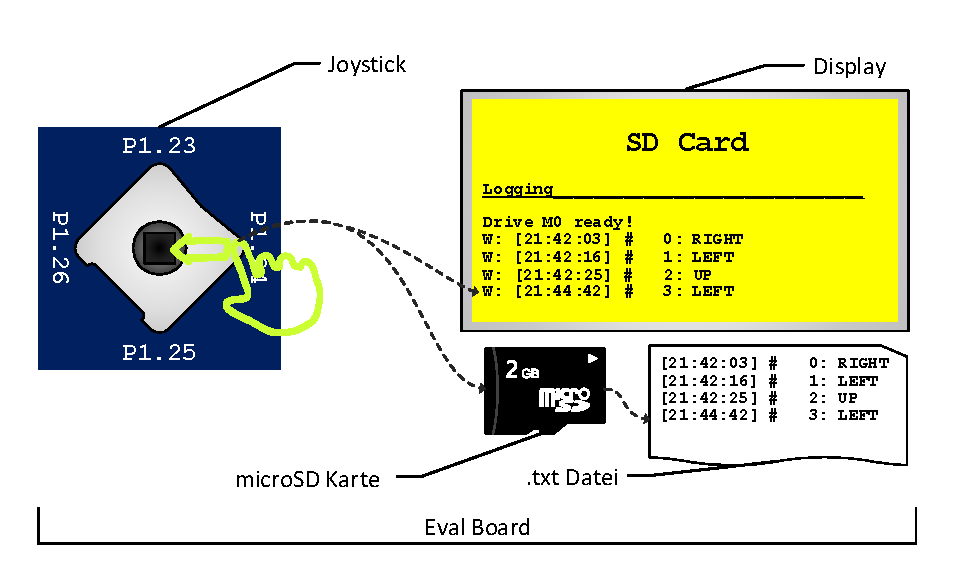
\includegraphics[width=1\textwidth]{images/SDCardSzenario.pdf}
		\caption{Beispielhaftes Logging der Joystick Position auf dem Display und auf der SD-Karte.}
	\label{fig:SDCardSzenario}
\end{figure}

Zus�tzlich ist es m�glich, auf den Joystick zu dr�cken, was im Folgenden als Richtung \textit{SELECT} bezeichnet wird. Die Richtung \textit{SELECT} soll eine besondere Funktion im Beispielszenario einnehmen. Dr�ckt der Benutzer den Joystick zweimal hintereinander, dann soll die SD-Karte die angelegte Log-Datei l�schen. Bei erstmaligem Dr�cken soll die SD-Karte dem Benutzer �ber das Display mitteilen, dass die SD-Karte durch erneutes Dr�cken des Joysticks die angelegte Log-Datei l�scht. W�hlt der Benutzer jedoch eine andere Richtung, soll die SD-Karte wieder in den Log-Status zur�ckkehren. Ebenso soll die SD-Karte eine minimale Fehlerbehandlung enthalten und dem Benutzer �ber das Display entsprechende Fehlermeldungen anzeigen.

Zur Verifizierung der Lesefunktion soll die SD-Karte �berpr�fen, ob bereits eine Log-Datei durch vorherige Verwendung angelegt wurde. Wenn das der Fall ist, soll die SD-Karte die letzte Zeile der Log-Datei auslesen, die fortlaufende Nummer extrahieren und den Z�hler auf diesen Wert setzen. 

\subsection{Architektur}

Das Klassendiagramm in \autoref{fig:ClassDiagramSDCard} stellt die Architektur des SD-Karten Loggings dar. Im Fokus des Diagramms steht die Klasse \texttt{SDCard}. Sie besitzt eine gerichtete Assoziation zur Klasse \texttt{Clock} und zur Klasse \texttt{Display}. Dadurch kann die Klasse \texttt{SDCard} einen Zeitstempel abfragen und den aktuellen Status auf dem Display ausgeben. 

\begin{figure}[!b]
	\centering
		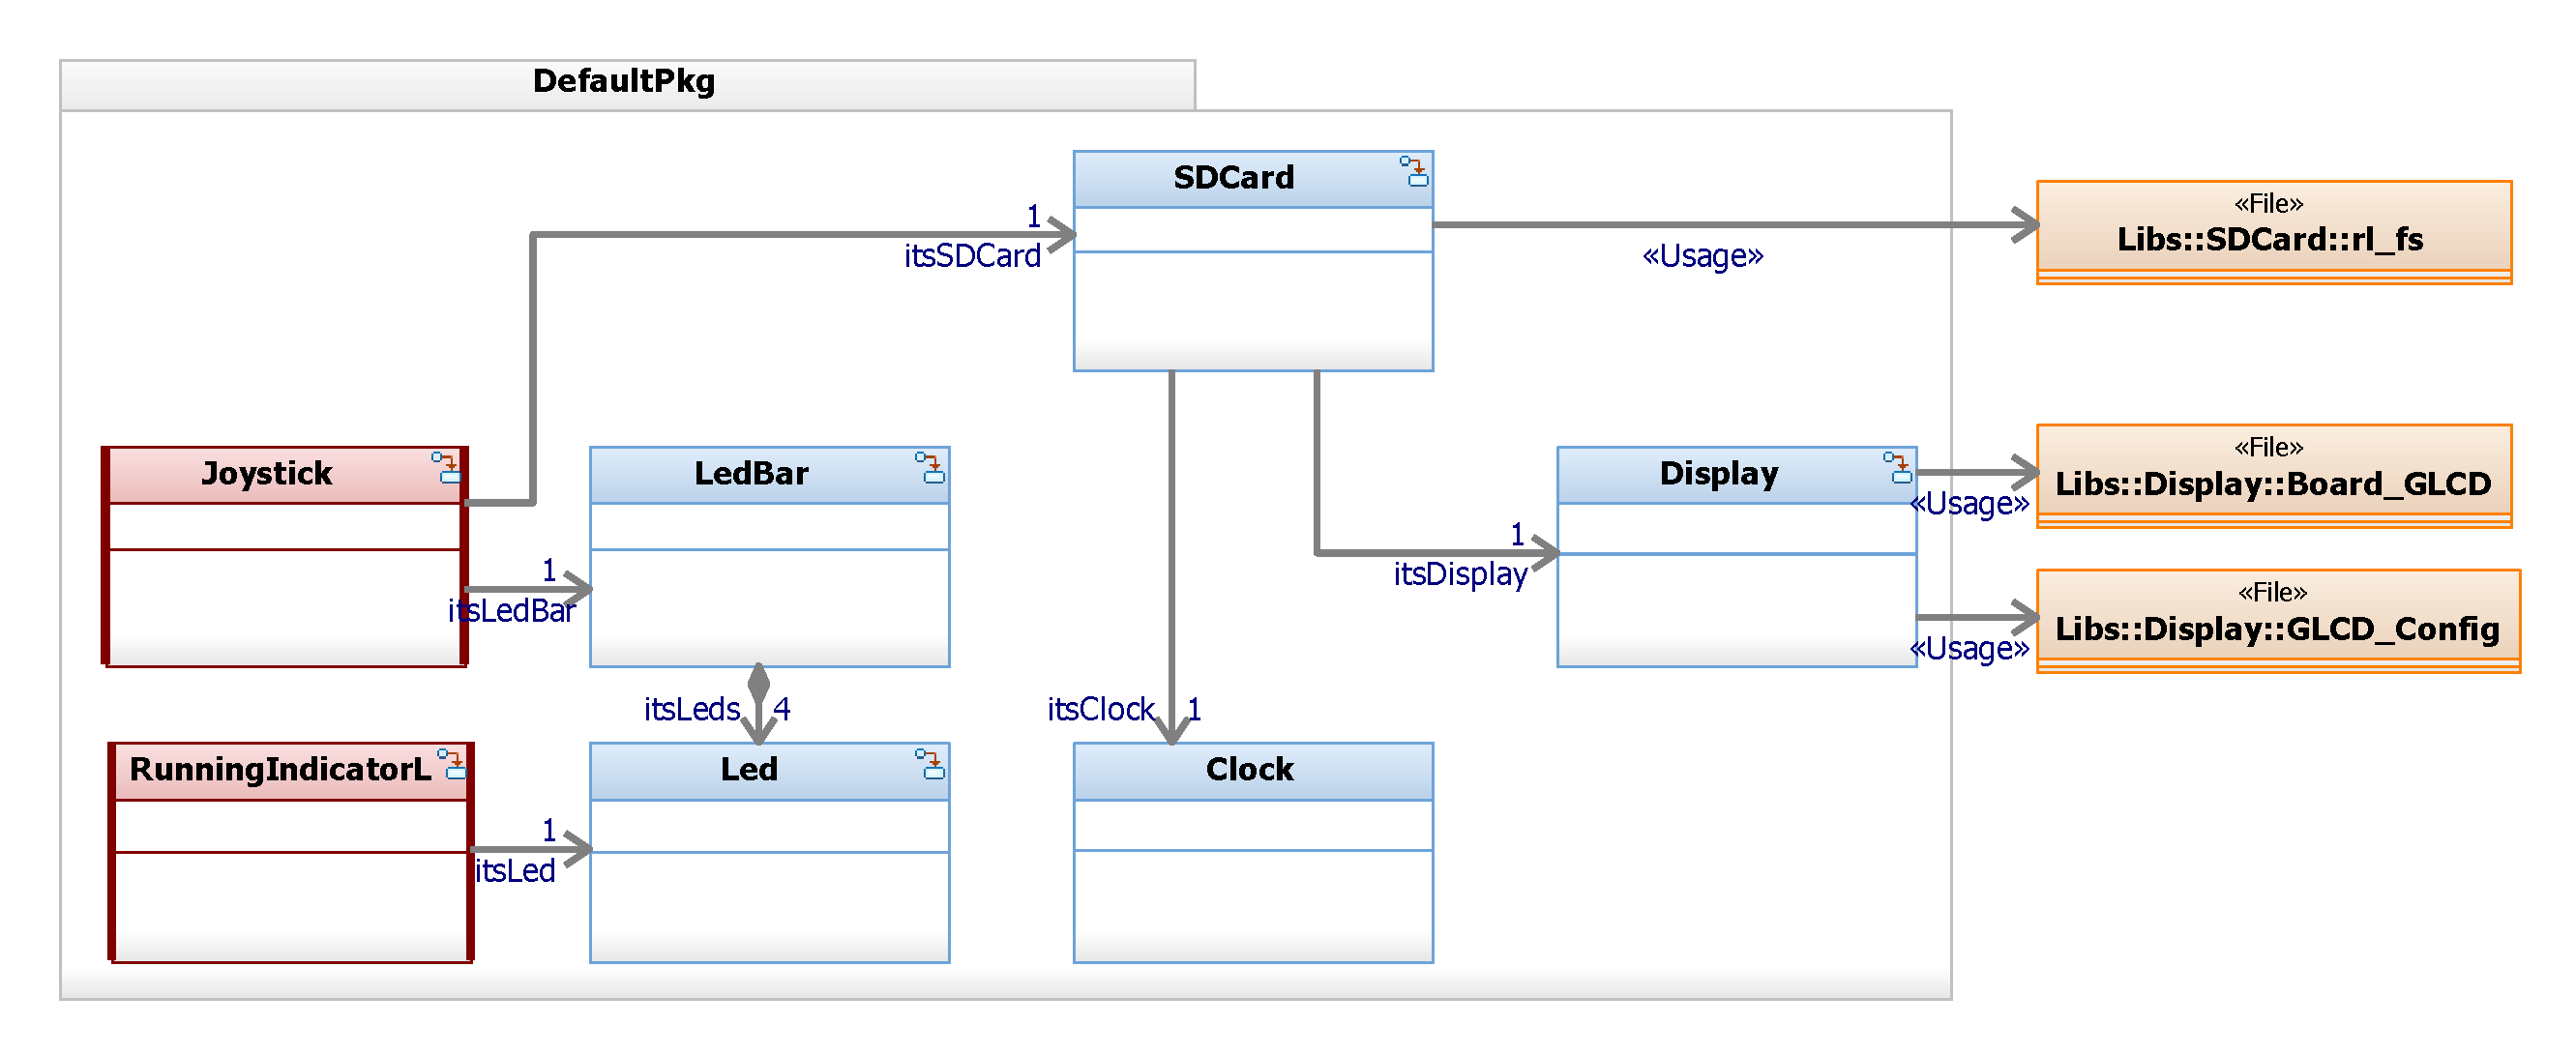
\includegraphics[width=1\textwidth]{images/ClassDiagramSDCard.pdf}
		\caption{Klassendiagramm zum Logging der Joystick Positionen auf der SD-Karte. Klassen, die in eigenen Threads laufen sind rot eingezeichnet.}
	\label{fig:ClassDiagramSDCard}
\end{figure}

In \autoref{fig:ClassDiagramSDCard} links dargestellt sind beiden Klassen \texttt{Jostick} und \texttt{Running\-Indicator\-Led}, welche in eigenen Threads laufen. Dabei verf�gt die Klasse \texttt{Jostick} �ber eine gerichtete Assoziation zur Klasse \texttt{SDCard}. Somit kann die Klasse \texttt{Joystick}, welche in einem festgelegten Intervall die Joystick Position pollt, die Klasse \texttt{SDCard} �ber Positions�nderungen informieren. Die Klasse \texttt{Joystick} verf�gt �ber eine weitere Assoziation zur Klasse \texttt{LedBar}, wodurch die Joystick Position mit Hilfe von vier LEDs visualisiert wird. Wie in den vorherigen Implementierungen l�sst die Klasse \texttt{Running\-Indicator\-Led} die LED P1.31 zyklisch blinken und dient lediglich zu Debugging zwecken. Die in \autoref{fig:ClassDiagramSDCard} rechts in orange dargestellten Dateien au�erhalb des Pakets \texttt{DefaultPkg} stellen Abh�ngigkeiten zu externen Bibliotheken dar. Die verwendeten Bibliotheken stammen aus der MDK Middleware und vereinfachen das Betreiben der File System und Graphics Component.

\subsection{Design und Coding}

Dieses Kapitel behandelt Attribute, Funktionen und Statecharts wichtiger Klassen.

\subsubsection*{SD-Karte}

Die Implementierung der SD-Karte erfolgt durch die MDK Middleware File System Component in der Version 6.9.8. Die File System Component unterst�tzt eine Vielzahl an Speichern und Speicherger�ten, welchen jeweils ein Laufwerksbuchstabe zugewiesen ist. Der Laufwerksbuchstabe wird an Systemroutinen �bergeben, wo er zur Initialisierung eines Dateisystems verwendet wird. Das Dateisystem, wie beispielsweise File Allocation Table (FAT) File System oder Embedded File System (EFS) wird in Abh�ngigkeit vom Laufwerk festgelegt. Die Klasse \texttt{SDCard} mit ihren Attributen und Operationen ist in \autoref{fig:SDCardClass} dargestellt. Dabei legt das Attribut \texttt{drive} den Laufwerksbuchstaben "`M0:"' und das damit verbundene Dateisystem FAT fest.

\begin{figure}[!b]
	\centering
		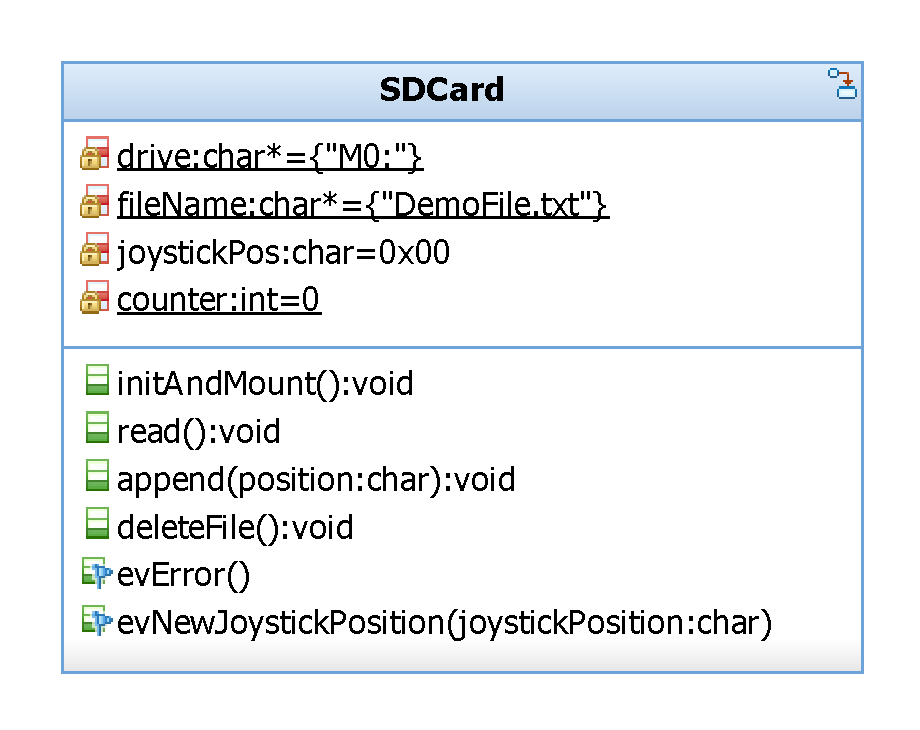
\includegraphics[width=0.5\textwidth]{images/SDCardClass.pdf}
		\caption{Klassendiagramm der SD-Karte.}
	\label{fig:SDCardClass}
\end{figure}

\paragraph{Initialisierung:}
Das Sequenzdiagramm in \autoref{fig:SDCardInit} stellt den Ablauf der Operation \texttt{init\-And\-Mount} dar. Dabei erfolgt das Initialisieren und Mounten des Dateisystems �ber die Systemroutinen \texttt{finit} und \texttt{fmount}. Au�erdem sind die entsprechenden Statusmeldungen an das Display im Erfolgsfall (gr�n) und Fehlerfall (rot) eingezeichnet.

\begin{figure}[!hbt]
	\centering
		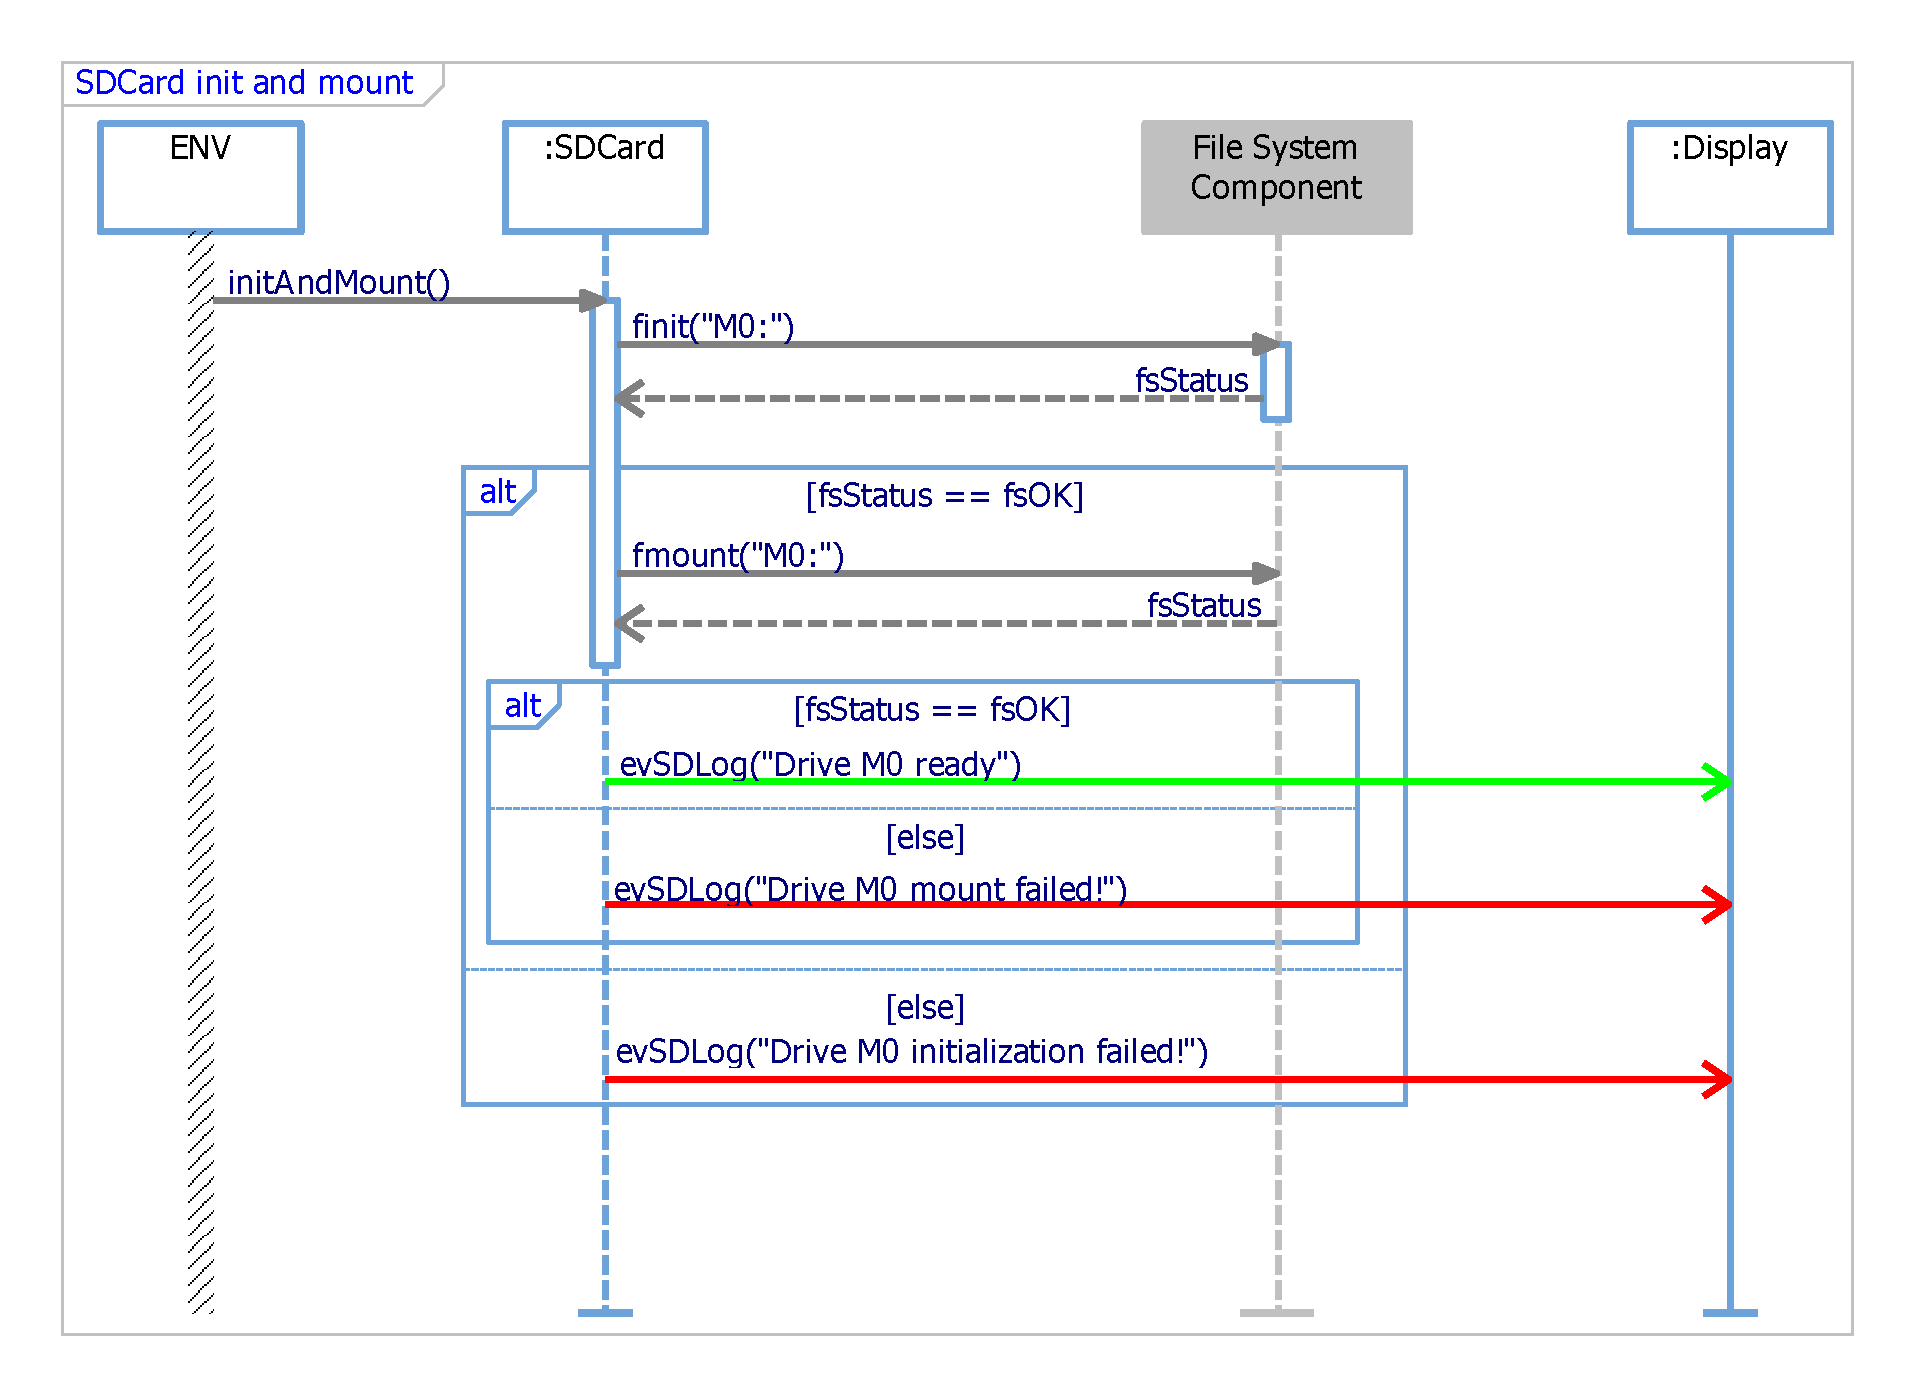
\includegraphics[width=1\textwidth]{images/SDCardInit.pdf}
		\caption{Initialisieren und Mounten der SD-Karte.}
	\label{fig:SDCardInit}
\end{figure}

\paragraph{Lesen:}
Leseoperationen erfolgen mit Hilfe der Standard Input und Output Library \texttt{stdio.h}. Die Library \texttt{stdio.h} benutzt Datenstr�me (Stream)zur Kommunikation mit physikalischen Peripherieger�ten wie Tastatur und Drucker, oder auch zur Kommunikation mit jeder anderen Art von Dateien, welche das System unterst�tzt. Dabei werden die Streams immer identisch angewendet, unabh�ngig davon, ob mit einem Ger�t oder einer Datei kommuniziert wird. Durch die Funktion \texttt{fopen} wird ein Stream ge�ffnet und mit einem Ger�t oder einer Datei verbunden. Bei erfolgreichem �ffnen des Streams gibt die Funktion \texttt{fopen} einen Zeiger auf ein FILE-Objekt zur�ck. Dieser Zeiger beinhaltet alle Informationen des Datenstroms und muss bei jeder weiteren Dateioperation als Parameter �bergeben werden.

Der f�r dieses Szenario implementierte Lese-Mechanismus ist als Sequenzdiagramm in \autoref{fig:SDCardRead} abgebildet. Nach dem �ffnen des Streams wird mit der Funktion \texttt{fgets} Zeile f�r Zeile aus der Log-Datei ausgelesen, bis das Ende der Datei erreicht ist. 

\begin{figure}[!hbt]
	\centering
		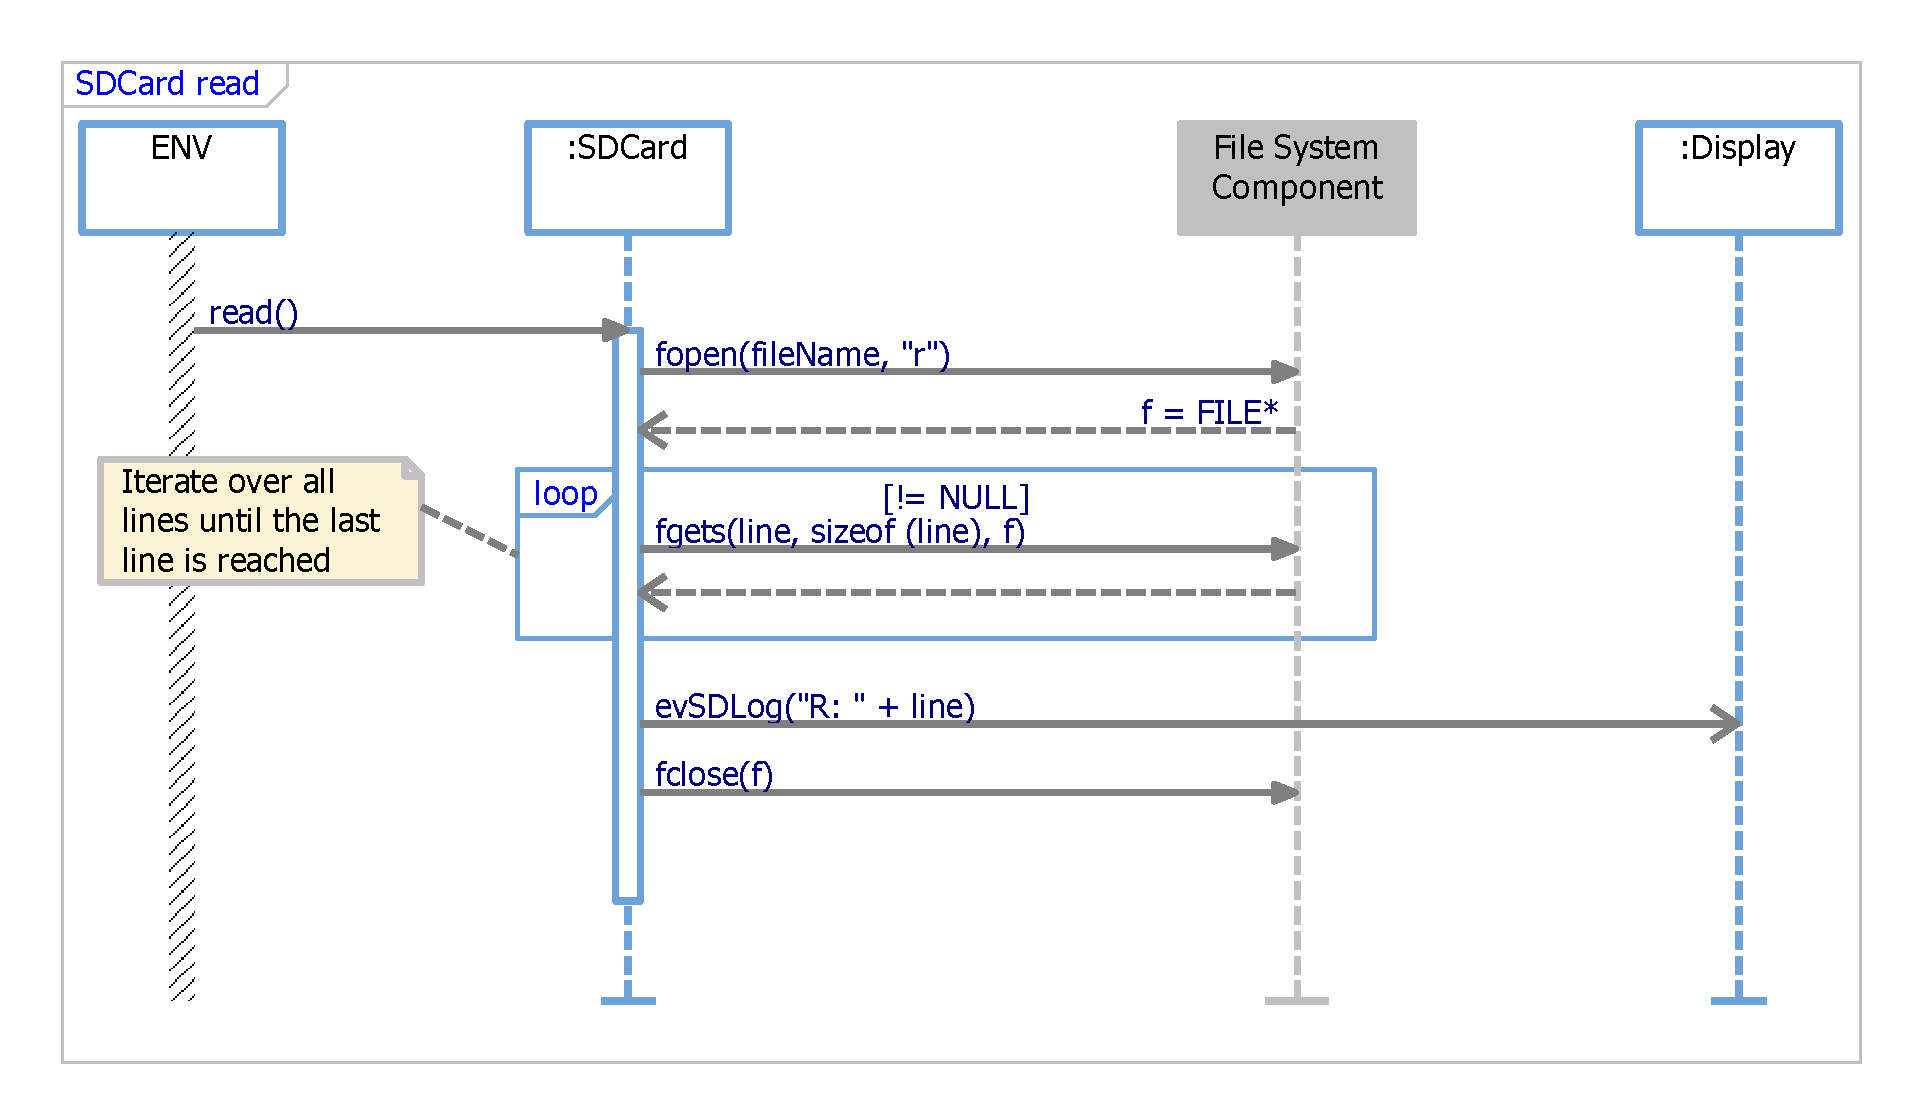
\includegraphics[width=1\textwidth]{images/SDCardRead.pdf}
		\caption{Lesen der SD-Karte.}
	\label{fig:SDCardRead}
\end{figure}

Da alle Zeilen der Log-Datei das gleiche Format haben, kann aus der letzten Zeile die fortlaufende Nummer extrahiert und zum Setzen des Z�hlers benutzt werden (siehe \autoref{fig:SDCardScenario1}). Den entsprechenden Ausschnitt aus der Operation \texttt{read} zeigt \autoref{lst:ExtractCounter}. Dabei wird zun�chst der Teil der Zeichenkette ab dem \#-Symbol extrahiert. Danach wird mit der Funktion \texttt{scanf} der Dezimalwert ausgelesen und in \texttt{counter} geschrieben. Im Anschluss wird das Event \texttt{evSDLog} mit der Bezeichnung "`R: "' f�r \textit{Read} und der letzten gelesenen Zeile als Parameter an das Display gefeuert, wie \autoref{fig:SDCardScenario2} zeigt. Nach erfolgter Dateioperation muss der Datenstrom wieder mittels \texttt{fclose} geschlossen werden.

\lstset{escapechar=@, escapeinside={(*@}{@*)}, style=customcpp}
\begin{lstlisting}[caption={Extrahieren des aktuellen Z�hlstandes aus dem Logfile.}, captionpos=b, label={lst:ExtractCounter}]
// Set counter to last value
substring = strstr(line, "# ");
if (substring != NULL)
{
	/* Found "# " in row. Extract decimal */
	sscanf(substring + 3, "%d", &counter);
}  
\end{lstlisting}

\paragraph{Schreiben:}
Wie die Leseoperationen bedienen sich auch die Schreiboperationen bei der Standard Input und Output Library \texttt{stdio.h}. Gleicherma�en gilt es zun�chst einen Stream zu �ffnen um einen Zeiger auf ein FILE-Objekt zu erhalten. Im Gegensatz zur Leseoperation, welche die Funktion \texttt{fopen} mit dem Parameter "`r"' f�r den \textit{Read mode} aufruft, wird bei der Schreiboperation der Parameter "`a"' f�r den \textit{Append mode} verwendet. Der \textit{Append mode} �ffnet eine bestehende Datei und f�gt dieser Inhalte hinzu. Falls die Datei noch nicht besteht, wird eine leere Datei angelegt. Wenn eine Datei im \textit{Append mode} ge�ffnet wird, werden die neuen Inhalte stets am Ende der Datei hinzugef�gt.

\begin{figure}[!b]
	\centering
		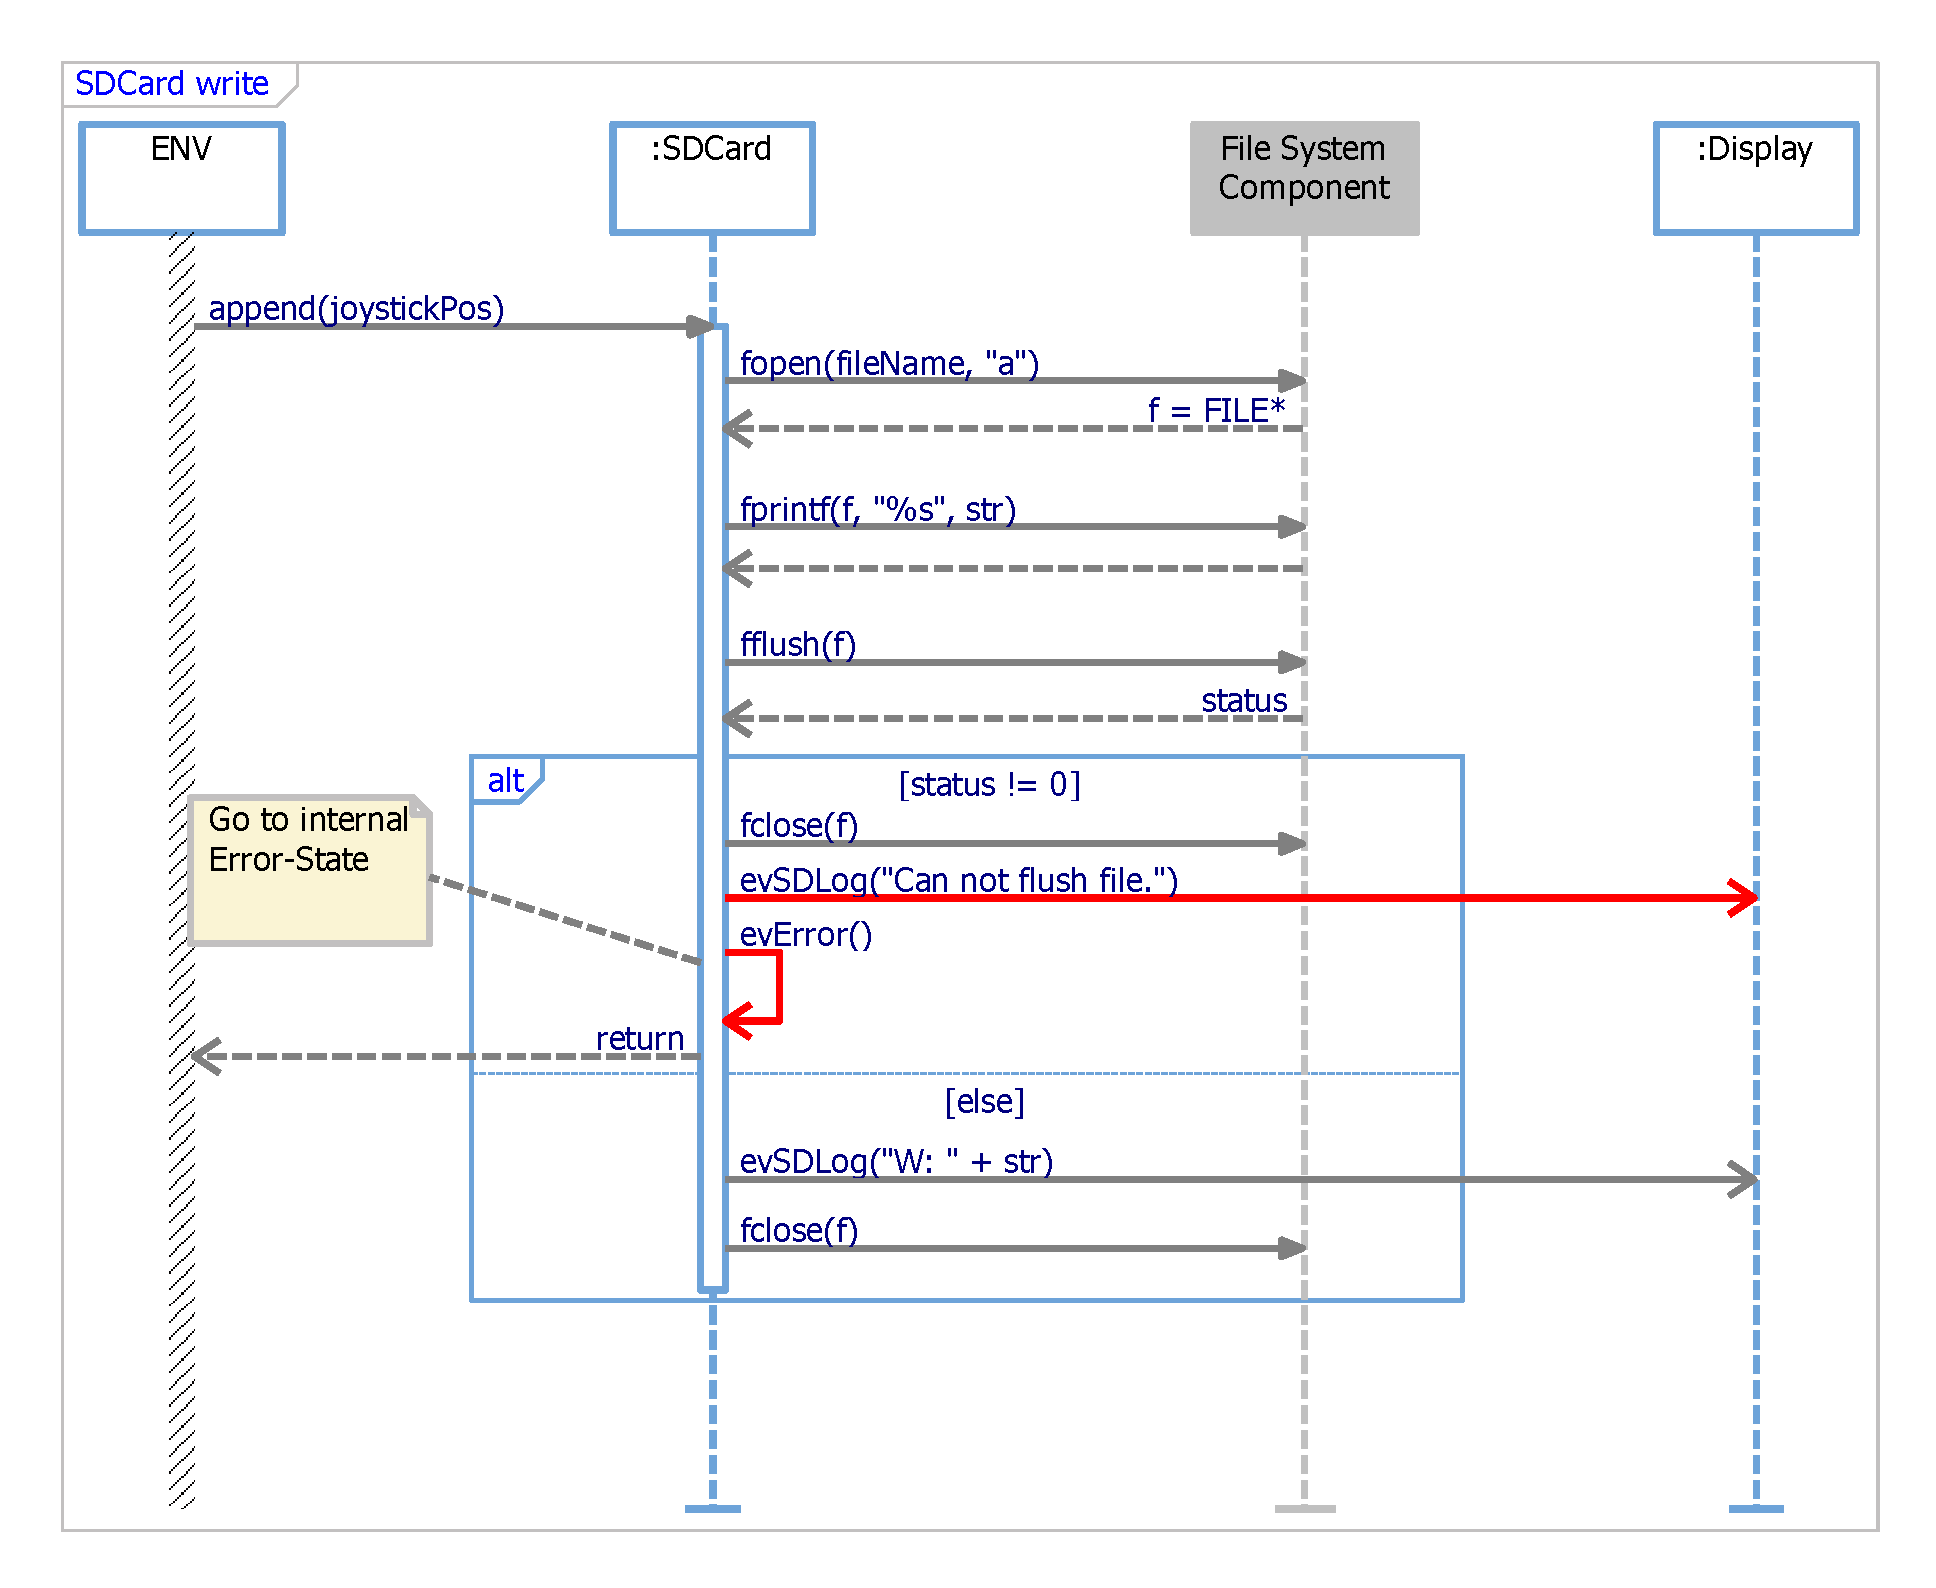
\includegraphics[width=1\textwidth]{images/SDCardWrite.pdf}
		\caption{Schreiben auf die SD-Karte.}
	\label{fig:SDCardWrite}
\end{figure}

Der implementierte Schreib-Mechanismus ist in \autoref{fig:SDCardWrite} als Sequenzdiagramm dargestellt. Nach dem �ffnen des Datenstroms wird die Zeichenkette \texttt{str}  durch die Funktion \texttt{fprintf} in den Stream geschrieben. Die Funktion \texttt{fflush} sorgt letztendlich daf�r, dass die Schreiboperation ausgef�hrt wird. Das bedeutet, dass die zugeh�rigen Buffer geleert und deren Inhalt in die entsprechende Datei geschrieben wird. Sollte der R�ckgabewert der Funktion \texttt{fflush} ungleich Null sein, so ist ein Fehler aufgetreten. Das ist beispielsweise dann der Fall, wenn keine SD-Karte im Slot eingelegt ist. Die Klasse \texttt{SDCard} feuert in diesem Fall das Event \texttt{evSDLog} mit einer entsprechenden Fehlermeldung an das Display, sowie das Event \texttt{evError} an sich selbst (siehe rote Markierungen in \autoref{fig:SDCardWrite}). Ausgel�st durch das Event \texttt{evError} f�hrt die Klasse \texttt{SDCard} eine entsprechende Fehlerbehandlung durch. Bei einer erfolgreichen Schreiboperation feuert die Klasse \texttt{SDCard} ebenfalls das Event \texttt{evSDLog} an das Display. In diesem Fall beinhaltet der Parameter des Events \texttt{evSDLog} den Bezeichner "`W: "' f�r \textit{Write} sowie die aktuell geschriebene Zeile. Zuletzt muss der Datenstrom durch die Funktion \texttt{fclose} wieder geschlossen werden.

\begin{figure}
	\centering
	\subfigure[Erstellen einer leeren Datei nach Reset und dreifache Schreiboperation.]{
					\label{fig:SDCardScenario1}
					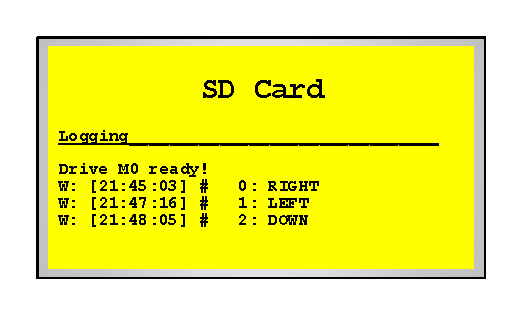
\includegraphics[width=0.45\textwidth]{images/SDCardScenario1.pdf}
	}
	\hfill 
	\subfigure[Auslesen einer bestehenden Datei nach einem Reset und einmaliges Schreiben.]{
					\label{fig:SDCardScenario2}
					\includegraphics[width=0.45\textwidth]{images/SDCardScenario2.pdf}
	}
	\subfigure[Erstmaliges Bet�tigen von SELECT fordert zum Wiederholen auf.]{
				\label{fig:SDCardScenario3}
				\includegraphics[width=0.45\textwidth]{images/SDCardScenario3.pdf}
	}
	\hfill 
	\subfigure[Erneutes Bet�tigen von SELECT l�scht die Datei.]{
					\label{fig:SDCardScenario4}
					\includegraphics[width=0.45\textwidth]{images/SDCardScenario4.pdf}
	}
	\caption{Verschiedene Statusausgaben auf dem Display.}
	\label{fig:SDCardStatusOnDisplay}
\end{figure}

\paragraph{Datei anlegen:}
Das Anlegen einer Datei geschieht implizit beim Aufruf der Funktion \texttt{fopen}. Dabei ist der �bergabeparameter f�r den Zugriffsmodus entscheidend. Mit "`a"' f�r \textit{Append mode} wird nur dann eine leere Datei angelegt, wenn diese noch nicht existiert. Mit dem Parameter "`w"' f�r \textit{Write mode} wird bei jedem Aufruf eine leere Datei angelegt. Eine existierende Datei wird dabei �berschrieben.

\paragraph{Datei l�schen:}
Zum L�schen einer Datei dient die Funktion \texttt{fdelete}. Als Parameter wird dieser Funktion der Name einer zu l�schenden Datei oder eines Verzeichnisses �bergeben. Mit einem weiteren Parameter "`/S"' wird spezifiziert, ob bei Angabe eines Verzeichnisses alle Dateien und Unterverzeichnisse ebenfalls gel�scht werden sollen. Die Funktion \texttt{fdelete} liefert einen R�ckgabewert vom Typ \texttt{fsStatus} der eine detaillierte Fehlerbehandlung erm�glicht. 

Die implementierte L�schprozedur im Rahmen des Beispielszenarios ist in \autoref{fig:SDCardStatechart} in gr�n gekennzeichnet. Zun�chst wird nach einem RESET des Targets die SD-Karte initialisiert und eine Leseoperation ausgef�hrt, so dass sich die SD-Karte im \textit{Read} State befindet. Der Trigger f�r nahez alle weiteren Transitionen ist das Event \texttt{evNewJoystickPosition}, welches von der Klasse \texttt{Joystick} abgefeuert wird. Bei jedem Empfangen wird ausgewertet, ob dessen Parameter der Richtung \textit{SELECT} entspricht. Ist das der Fall, so geht die SD-Karte in die L�schprozedur �ber, indem zun�chst der State \textit{Confirm\_Delete} aktiviert wird. In diesem State feuert die Klasse \texttt{SDCard} das Event \texttt{evSDLog} an das Display, wodurch der Benutzer zum erneuten Bet�tigen der Richtung \textit{SELECT} aufgefordert wird (siehe \autoref{fig:SDCardScenario3}). Triff wiederholt ein Event mit der Richtung \textit{SELECT} als Parameter ein, wird schlie�lich der State \textit{Delete\_File} eingenommen. Das f�hrt letztendlich zum Aufruf der Operation \texttt{deleteFile}. Wenn der Parameter des Events \texttt{evNewJoystickPosition} ungleich der Richtung \textit{SELECT} ist, kehrt die SD-Karte immer in den \textit{Log} State zur�ck.

\begin{figure}[!b]
	\centering
		\includegraphics[width=0.9\textwidth]{images/SDCardStatechart.pdf}
		\caption{Statechart zum Initialisieren, Lesen und Schreiben der SD-Karte (blau), sowie zum L�schen einer Datei (gr�n).}
	\label{fig:SDCardStatechart}
\end{figure}

\subsubsection*{Joystick}
Die Implementierung des Joysticks entspricht im Wesentlichen der Umsetzung aus \autoref{subsec:EthDesignUndCoding}, mit der Erg�nzung, dass an dieser Stelle auch die Richtung \textit{SELECT} ausgewertet wird. Dazu ist es n�tig, \autoref{joystickPosition} in \autoref{lst:JoystickFilter} auszukommentieren, so dass erweiterte Richtungsinformationen vorhanden sind. Durch die erweiterten Richtungsinformationen ergeben sich dementsprechend andere Bitmuster, was eine Anpassung der Enumeration \texttt{DIRECTION} erfordert. Ein weiterer Unterschied ist, dass die Klasse \texttt{Joystick} bei jeder neuen Richtung das Event \texttt{evNewJoystickPosition} an die Klasse \texttt{SDCard} sendet.

\subsubsection*{Clock}
Da ein Logging nur dann Sinn macht, wenn es auch mit einem Zeitstempel versehen ist, wurde die Klasse \texttt{Clock} implementiert. Sie greift auf die Real-Time Clock (RTC) \abk{$RTC$}{Real-Time Clock} des Keil MCB1760 Eval Boards zu. Die Prozedur zur Initialisierung der RTC ist in \autoref{lst:RTC} dargestellt. Hier ist zu beachten, dass die auskommentierten Bl�cke von \autoref{cdl:line12} bis \autoref{cdl:line14} und \autoref{cdl:line17} bis \autoref{cdl:line19} einmalig vor dem Flashen des Targets einkommentiert und entsprechend aktualisiert werden m�ssen. Damit wird das Datum und die Uhrzeit des Targets eingestellt und bleibt solange aktuell, bis das Target von der Spannungsversorgung getrennt wird. Zur Ermittlung der Uhrzeit liest die Klasse \texttt{Clock} die entsprechenden Register aus und stellt deren Inhalt �ber Operationen \texttt{getHour}, \texttt{getMin} und \texttt{getSec} zur Verf�gung \parencite[S. 558 ff]{LPC17xxUserManual2010}.

\lstset{escapechar=@, escapeinside={(*@}{@*)}, style=customcpp}
\begin{lstlisting}[caption={Initialisierung der RTC.}, captionpos=b, label={lst:RTC}]
/* Enable CLOCK into RTC */
LPC_SC->PCONP |= (1 << 9);

/* Disable RTC clock, reset clock, Enable RTC calibration */
LPC_RTC->CCR = ((1 << SBIT_CTCRST ) | (1 << SBIT_CCALEN));
LPC_RTC->CALIBRATION = 0x00;
LPC_RTC->CCR = (1 << SBIT_CLKEN);    /* Enable the clock for RTC */

// Set Date and Time only once
// Comment these lines after setting the time and date                                           
// Set Date 29th May 2017 
//LPC_RTC->DOM    = 29;   // Update date value (*@\label{cdl:line12}@*)
//LPC_RTC->MONTH  = 5;    // Update month value
//LPC_RTC->YEAR   = 2017; // Update year value (*@\label{cdl:line14}@*)

// Set Time 22:05:25 AM 
//LPC_RTC->HOUR   = 22;   // Update hour value (*@\label{cdl:line17}@*)
//LPC_RTC->MIN    = 05;   // Update min value
//LPC_RTC->SEC    = 25;   // Update sec value (*@\label{cdl:line19}@*)
\end{lstlisting}

\subsubsection*{Display}

Das Display dient in diesem Szenario als Statusanzeige und soll �ber erfolgreiche Lese- und Schreiboperationen informieren, sowie auch Fehlermeldungen darstellen. Dazu soll das Display das Funktionsprinzip einer Kommandozeile nachahmen, in welcher das neuste Ereignis an unterster Stelle hinzugef�gt wird. Beim Erreichen der maximalen Zeilenanzahl sollen folglich alle Zeilen um eine Position nach oben geschoben werden, was dazu f�hrt, dass die oberste Zeile entfernt wird. Die maximale Zeilenanzahl wird �ber das Attribut \texttt{maxLoggedLines} festgelegt und hat initial den Wert sieben. Das Funktionsprinzip ist beispielhaft f�r eine maximale Zeilenanzahl von f�nf in \autoref{fig:SDCardConsoleOnDisplay} dargestellt.
\begin{figure}[!b]
	\centering
	\subfigure[Neues Ereignis tritt ein. Zeile wird unten hinzugef�gt. Maximale Zeilenanzahl erreicht.]{
					\label{fig:SDCardConsole1}
					\includegraphics[width=0.45\textwidth]{images/SDCardConsole1.pdf}
	}
	\hfill 
	\subfigure[Neues Ereignis tritt ein. Oberste Zeile wird gel�scht. All weiteren Zeilen werden eine Position nach oben geschoben.]{
					\label{fig:SDCardConsole2}
					\includegraphics[width=0.45\textwidth]{images/SDCardConsole2.pdf}
	}
	\subfigure[Neue Zeile wird unten hinzugef�gt. Neues Ereignis tritt ein. Oberste Zeile wird gel�scht. All weiteren Zeilen werden eine Position nach oben geschoben.]{
				\label{fig:SDCardConsole3}
				\includegraphics[width=0.45\textwidth]{images/SDCardConsole3.pdf}
	}
	\hfill 
	\subfigure[Neue Zeile wird unten hinzugef�gt.]{
					\label{fig:SDCardConsole4}
					\includegraphics[width=0.45\textwidth]{images/SDCardConsole4.pdf}
	}
	\caption{Funktionsprinzip einer Kommandozeile auf dem Display. Das neuste Ereignis wird immer an unterster Stelle hinzugef�gt (gr�ner Rahmen). Wird eine maximale Zeilenanzahl erreicht, wird die oberster Zeile gel�scht (rote Linie). Alle anderen Zeilen werden um eine Position nach oben geschoben (gr�ner Pfeil).}
	\label{fig:SDCardConsoleOnDisplay}
\end{figure}

\subsection{Konfigurieren des Keil Projekts}

Ebenso wie in der Ethernet-Applikation in \autoref{sec:Ethernet} wird das Blinky"=Beispielprojekt aus dem RXF \textit{Rpy\_CPP\_CMSIS\_Keil5\_ARM\_MCB1700\_TD} von Willert eingesetzt. Somit ist eine lauff�hige Entwicklungsumgebung von Rational Rhapsody �ber das Willert RXF bis zur IDE Keil uVision hergestellt. Im Weiteren werden die wichtigsten Anpassungen in Konfiguration des Keil Projekts beschrieben.

\subsubsection*{Manage Run-Time Environment} 

Zur Verwendung der SD-Karte ist es n�tig, dem Keil Projekt mit Hilfe des Konfigurationsassistenten \includegraphics[width=0.3cm]{images/package.pdf} \textit{Manage Run"=Time Environment}, Software Komponenten hinzuzuf�gen. Zuallererst wird der Software Pack \textit{Keil::MDK"=Middleware} in der Version 7.4.1 (2017-04-21) dem Projekt hinzugef�gt. In diesem Paket ist die File System Component in der Version 6.9.8 (2017-04-21) enthalten. Zur Verwendung der File System Component wird der \textit{ARM::CMSIS:CORE} in der Version 5.0.1 ben�tigt. Zwar erstellt die File System Component keinen eigenen Thread, greift aber dennoch auf die Schnittstellen des Betriebssystems zu. Das geschieht beispielsweise dann, wenn eine Datei ge�ffnet wird und mittels Mutex ein exklusiver Zugriff auf die Datei gew�hrleistet wird. Die entsprechende Anpassung in der Run-Time Environment ist in \autoref{tab:RuntimeEnvSdCard} rot markiert.

Die File System Component unterst�tzt sowohl das Betreiben rudiment�rer Flash-Speicher-Chips in NAND- oder NOR-Architektur, als auch den Datenaustausch mit einem USB Massenspeicher oder einer SD Speicherkarte. Die ben�tigten Komponenten der File System Component f�r den Einsatz der SD Speicherkarte sind in \autoref{tab:RuntimeEnvSdCard} gelb gekennzeichnet. 

\begin{table}[!ht]
\centering
\footnotesize
\begin{tabular}{p{0.01mm}p{4.6cm}p{0.2cm}p{2.2cm}lp{0.2cm}p{2.2cm}l}
	\toprule
	& & \multicolumn{3}{ c }{Blinky} & \multicolumn{3}{ c }{SD Card} \\ \cmidrule{3-5}  \cmidrule{6-8}
	& Software Component & Sel. & Variant & Version & Sel. & Variant & Version \\
	\midrule
	& $\boxminus$\textSFx \includegraphics[width=0.25cm]{images/package.pdf} Board Support & & \tiny{MCB1700} & 1.0.0 & \cellcolor{KeilGreen} & \tiny{MCB1700} & 1.0.0 \\
	& \textSFxi\hspace{2ex}$\boxminus$\textSFx \includegraphics[width=0.25cm]{images/package.pdf} Graphic LCD (API) &  &  & 1.0.0 & \cellcolor{KeilGreen} &  & 1.0.0 \\
	\textcolor{Orange}{ \pmboxdrawuni{258E}} & \textSFxi\hspace{2ex}\textSFii\textSFx\textSFx	\includegraphics[width=0.2cm]{images/item.pdf} Graphic LCD & \HollowBox &  & 1.0.0 & \cellcolor{KeilGreen}\CheckedBox &  & 5.0.1 \\
	& $\boxminus$\textSFx \includegraphics[width=0.25cm]{images/package.pdf} CMSIS & \cellcolor{KeilGreen} & & & \cellcolor{KeilGreen} & & \\
	\textcolor{Red}{ \pmboxdrawuni{258E}} & \textSFxi\hspace{2ex}\textSFii\textSFx\textSFx	\includegraphics[width=0.2cm]{images/item.pdf} CORE & \cellcolor{KeilGreen}\CheckedBox  &  & 4.3.0 & \cellcolor{KeilGreen}\CheckedBox &  & 5.0.1 \\
	& $\boxminus$\textSFx \includegraphics[width=0.25cm]{images/package.pdf} CMSIS Driver & & & & \cellcolor{KeilGreen} & & \\
	& \textSFxi\hspace{2ex}$\boxminus$\textSFx \includegraphics[width=0.25cm]{images/package.pdf} SPI (API) & & & 2.01 & \cellcolor{KeilGreen} &  & 2.2.0 \\
	& \textSFxi\hspace{5ex}\textSFviii\textSFx\textSFx \includegraphics[width=0.20cm]{images/item.pdf} SPI & \HollowBox  &  & 2.1 & \HollowBox &  & 2.1.0 \\
	\textcolor{Yellow}{ \pmboxdrawuni{258E}} & \textSFxi\hspace{5ex}\textSFii\textSFx\textSFx \includegraphics[width=0.20cm]{images/item.pdf} SSP & \HollowBox  &  & 2.5 & \cellcolor{KeilGreen}\CheckedBox &  & 2.7.0 \\
	& $\boxminus$\textSFx \includegraphics[width=0.25cm]{images/package.pdf} Compiler & & \tiny{ARM Compiler} & 1.2.0 & \cellcolor{KeilGreen} & \tiny{ARM Compiler} & 1.2.0 \\
	& \textSFxi\hspace{2ex}\textSFviii\textSFx\textSFx \includegraphics[width=0.20cm]{images/item.pdf} Event Recorder & \HollowBox  & \tiny{DAP} & 1.1.0 & \HollowBox & \tiny{DAP} & 1.1.0 \\
	& \textSFxi\hspace{2ex}$\boxminus$\textSFx \includegraphics[width=0.25cm]{images/package.pdf} I/O &  &  & & \cellcolor{KeilGreen} &  & \\
	\textcolor{Yellow}{ \pmboxdrawuni{258E}} & \textSFxi\hspace{5ex}\textSFviii\textSFx\textSFx \includegraphics[width=0.20cm]{images/item.pdf} File & \HollowBox & \tiny{File System} & 1.2.0 & \cellcolor{KeilGreen} \CheckedBox & \tiny{File System} & 1.2.0 \\
	& \textSFxi\hspace{5ex}\textSFviii\textSFx\textSFx \includegraphics[width=0.20cm]{images/item.pdf} STDERR & \HollowBox & \tiny{User} & 1.2.0 & \HollowBox & \tiny{User} & 1.2.0 \\
	& \textSFxi\hspace{5ex}\textSFviii\textSFx\textSFx \includegraphics[width=0.20cm]{images/item.pdf} STDIN & \HollowBox & \tiny{User} & 1.2.0 & \HollowBox & \tiny{User} & 1.2.0 \\
	& \textSFxi\hspace{5ex}\textSFviii\textSFx\textSFx \includegraphics[width=0.20cm]{images/item.pdf} STDOUT & \HollowBox & \tiny{User} & 1.2.0 & \HollowBox & \tiny{User} & 1.2.0 \\
	& \textSFxi\hspace{5ex}\textSFviii\textSFx\textSFx \includegraphics[width=0.20cm]{images/item.pdf} TTY & \HollowBox & \tiny{User} & 1.2.0 & \HollowBox & \tiny{User} & 1.2.0 \\
	& $\boxminus$\textSFx \includegraphics[width=0.25cm]{images/package.pdf} Device & & & & \cellcolor{KeilGreen} & & \\
	\textcolor{Yellow}{ \pmboxdrawuni{258E}} & \textSFxi\hspace{2ex}\textSFviii\textSFx\textSFx \includegraphics[width=0.20cm]{images/item.pdf} GPDMA & \HollowBox &  & 1.2 & \cellcolor{KeilGreen}\CheckedBox &  & 1.2.0 \\
	\textcolor{Yellow}{ \pmboxdrawuni{258E}} & \textSFxi\hspace{2ex}\textSFviii\textSFx\textSFx \includegraphics[width=0.20cm]{images/item.pdf} GPIO & \HollowBox &  & 1.1 & \cellcolor{KeilGreen}\CheckedBox &  & 1.1.0 \\
	\textcolor{Yellow}{ \pmboxdrawuni{258E}} & \textSFxi\hspace{2ex}\textSFviii\textSFx\textSFx \includegraphics[width=0.20cm]{images/item.pdf} PIN & \HollowBox &  & 1.0 & \cellcolor{KeilGreen}\CheckedBox &  & 1.0.0 \\
	& \textSFxi\hspace{2ex}\textSFii\textSFx\textSFx \includegraphics[width=0.20cm]{images/item.pdf} Startup & \cellcolor{KeilGreen}\CheckedBox &  & 1.0.0 & \cellcolor{KeilGreen}\CheckedBox &  & 1.0.0 \\
	& $\boxminus$\textSFx \includegraphics[width=0.25cm]{images/package.pdf} File System & & \tiny{MDK-Pro} & 6.9.8 & \cellcolor{KeilGreen} & \tiny{MDK-Pro} & 6.9.8 \\
	\textcolor{Yellow}{ \pmboxdrawuni{258E}} & \hspace{3.2ex}\textSFviii\textSFx\textSFx \includegraphics[width=0.20cm]{images/item.pdf} CORE & \HollowBox & \tiny{SFN} & 6.9.8 & \cellcolor{KeilGreen}\CheckedBox & \tiny{LFN} & 6.9.8 \\
	& \hspace{3.2ex}$\boxminus$\textSFx \includegraphics[width=0.25cm]{images/package.pdf} Drive & & & & \cellcolor{KeilGreen} &  & \\
	\textcolor{Yellow}{ \pmboxdrawuni{258E}} & \hspace{3.2ex}\textSFxi\hspace{2ex}\textSFviii\textSFx\textSFx \includegraphics[width=0.20cm]{images/items.pdf} Memory Card & 0  &  & 6.9.8 & \cellcolor{KeilGreen} 1 &  & 6.9.8 \\
	& \hspace{3.2ex}\textSFxi\hspace{2ex}\textSFviii\textSFx\textSFx \includegraphics[width=0.20cm]{images/items.pdf} NAND & 0  &  & 6.9.8 & 0 &  & 6.9.8 \\
	& \hspace{3.2ex}\textSFxi\hspace{2ex}\textSFviii\textSFx\textSFx \includegraphics[width=0.20cm]{images/items.pdf} NOR & 0  &  & 6.9.8 & 0 &  & 6.9.8 \\
	& \hspace{3.2ex}\textSFxi\hspace{2ex}\textSFviii\textSFx\textSFx \includegraphics[width=0.20cm]{images/item.pdf} RAM & \HollowBox &  & 6.9.8 & \HollowBox &  & 6.9.8 \\
	& \hspace{3.2ex}\textSFxi\hspace{2ex}\textSFviii\textSFx\textSFx \includegraphics[width=0.20cm]{images/items.pdf} USB & 0  &  & 6.9.8 & 0 &  & 6.9.8 \\
	\bottomrule
\end{tabular}
\caption{Heraufsetzen des CMSIS:CORE (rot), ben�tigte Komponenten der File System Component und deren Abh�ngigkeiten (gelb), sowie die Komponenten zum Betreiben des Displays (orange).}
\label{tab:RuntimeEnvSdCard}
\end{table}

\subsubsection*{CMSIS Configuration} 

Die CMSIS Configuration behandelt die Einstellung des CMSIS RTX Kernel. Zwar legt die File System Component keine neuen Threads an, ben�tigt aber dennoch das CMSIS-RTOS zum Betrieb. Beispielsweise werden die Mechanismen zum Erstellen eines Mutex verwendet. Die Anforderungen an den CMSIS RTX Kernel werden in der Datei \textit{RTX\_Conf\_CM.c} eingepflegt, welche Teil der CMSIS Component ist. Diese Datei kann �ber den \textit{Configuration Wizard} von Keil editiert werden. Im Abschnitt \textit{Thread Configuration} in der Datei \textit{RTX\_Conf\_CM.c} spezifiziert der erste Parameter \textit{Number of concurrently running user threads} die Anzahl nebenl�ufiger Tasks. Die Tasks der SD-Karten Applikation sind in \autoref{tab:DefaultThreadsSDCard} aufgelistet. Dabei sind die Tasks mit der Ursache CMSIS-RTOS und Willert RXF identisch zu den Tasks in \autoref{tab:DefaultThreads} aus der Ethernet-Applikation. 

\begin{table}[!hbt]
\centering
\footnotesize
	\begin{tabular}{lcl}
	\toprule
	Task Name & Priorit�t & Ursache \\
	\midrule
	osTimerThread & 1 & CMSIS-RTOS \\
	main & 2 & CMSIS-RTOS \\
	os\_idle\_demon & 255 & CMSIS-RTOS \\
	WST\_\-Monitor\_receiveTask & 3 & Willert RXF \\
	RunningIndicator & 4 & SD-Karte Applikation \\
	Joystick & 5 & SD-Karte Applikation \\
	\bottomrule
	\end{tabular}
\caption{Verwendete Task f�r den Betrieb der SD-Karte und deren Ursache.}
\label{tab:DefaultThreadsSDCard}
\end{table}

Gem�� \citet{CmsisRtos2017} geht der Task \textit{os\_idle\_demon} nicht in die Anzahl der gleichzeitig laufenden Tasks mit ein, weshalb der Parameter \textit{Number of concurrent running user threads} auf den Wert f�nf gesetzt wird. Dementsprechend ist auch der Parameter \textit{Number of threads with user-provided stack size} auf den Wert vier zu setzen, da hier der main-Task nicht mitgez�hlt wird. 

Abh�ngig vom gew�hlten Drive Type gibt \citet{FileSystemComponentResourceRequirements2017} vor, wie die Parameter bez�glich der \textit{Default}, \textit{Main} und \textit{Total Thread stack size} zu konfigurieren sind. F�r den hier gew�hlten Drive Type \textit{Memory Card drive 0} in Kombination mit dem CMSIS Treiber f�r SPI sind keine weiteren Anpassung n�tig. Die �nderungen in der Datei \textit{RTX\_Conf\_CM.c} gegen�ber dem Blinky-Projekt sind in \autoref{tab:RtxConfigSDCard} zusammengefasst.

\begin{table}[!htb]
\footnotesize
\centering
	\begin{tabular}{p{7.6cm}p{3.0cm}p{3.0cm}}
	\toprule
	& Blinky & SD-Karte \\ \cmidrule{2-3}
	Option & Value & Value \\
	\midrule
	$\boxminus$\textSFx Thread Configuration & &  \\
	\textSFxi\hspace{2ex}\textSFviii\textSFx\textSFx Number of concurrent running user threads & 6 & 5 (-1) \\
	\textSFxi\hspace{2ex}\textSFviii\textSFx\textSFx Default Thread stack size [bytes] & 200 & 200 \\
	\textSFxi\hspace{2ex}\textSFviii\textSFx\textSFx Main Thread stack size [bytes] & 1024 & 1024 \\
	\textSFxi\hspace{2ex}\textSFviii\textSFx\textSFx Number of threads with user-provided & 5 & 4 (-1) \\
	\textSFxi\hspace{2ex}\textSFxi \hspace{1.5ex} stack size &  & \\
	\textSFxi\hspace{2ex}\textSFviii\textSFx\textSFx Total stack size [bytes] for threads with & 4096 & 5632 (+1536)\\
	\textSFxi\hspace{2ex}\textSFxi \hspace{1.5ex} user-provided stack size &  & \\
	\textSFxi\hspace{2ex}\textSFviii\textSFx\textSFx  Check for stack overflow & \CheckedBox &  \CheckedBox \\
	\textSFxi\hspace{2ex}\textSFii\textSFx\textSFx  Processor mode for thread execution & Privileged mode & Privileged mode \\
	$\boxplus$\textSFx RTX Kernel Timer Tick Configuration & & \\
	$\boxplus$\textSFx System Configuration & & \\
	\bottomrule
	\end{tabular}
\caption{Anpassungen in der RTX Configuration \textit{RTX\_Conf\_CM.c} f�r die SD-Karte.}
\label{tab:RtxConfigSDCard}
\end{table}

Der Vollst�ndigkeit halber wird an dieser Stelle noch auf die Anforderungen bez�glich Mutexes eingegangen, auch wenn im Rahmen dieser Implementierung keine Anpassung n�tig sind. Sollen mehr als drei Dateien gleichzeitig ge�ffnet und bearbeitet werden, muss die Anzahl der Mutexobjekte angepasst werden. Diese �nderung kann nicht �ber den \textit{Configuration Wizard} erfolgen, sondern muss direkt in der Datei \textit{RTX\_Conf\_CM.c} manuell durchgef�hrt werden. Dabei ist der Parameter \textit{OS\_MUTEXCNT} zu editieren, welcher standardm��ig auf den Wert acht gesetzt ist. Der Parameter \textit{OS\_MUTEXCNT} setzt sich dabei folgenderma�en zusammen: 2 (internal stdio operations) + 3 (stdin, stdout und stderr file streams) + 3 f�r jede ge�ffnete Datei.

\subsubsection*{Device Configuration}

Die Dateien \textit{startup\_LPC17xx.s (Startup)}, \textit{startup\_LPC17xx.c (Startup)} und\linebreak \textit{RTE\_Device.h (Startup)} implementieren den Start-up Code, welcher direkt nach einem RESET des Targets ausgef�hrt wird. Alle drei Dateien geh�ren zur Device Component und k�nnen ebenfalls �ber den \textit{Configuration Wizard} bearbeitet werden. Von gr��erem Interesse ist zun�chst die Datei \textit{startup\_LPC17xx.s (Startup)} bei der festgelegt wird, wie viel Speicher f�r Stack und Heap zu reservieren sind.

Bei Verwendung der File System Component ist eine Vergr��erung der Stack Size um 512 Bytes n�tig. Eine Anpassung des Heaps ist ebenfalls erforderlich und h�ngt dabei mit der Anzahl gleichzeitig ge�ffneter Dateien zusammen. F�r jede ge�ffnete Datei m�ssen 512+96 Bytes reserviert werden. In diesem Fall soll nur eine Datei gleichzeitig ge�ffnet werden \parencite{FileSystemComponentResourceRequirements2017}.  Wie \autoref{tab:StartupConfigSDCard} zu entnehmen ist, wurde der Heap insgesamt um 4096 Bytes vergr��ert. Die Differenz von 3488 Bytes kommt f�r den Betrieb des Logging-Mechanismus auf dem Display zum Einsatz. Dieser Mechanismus basiert auf der Klasse \texttt{OMString}, welche Teil des Rhapsody OXF ist und zus�tlichen Heap ben�tigt.

\begin{table}[!hbt]
\footnotesize
\centering
	\begin{tabular}{p{7.6cm}p{3.0cm}p{3.0cm}}
	\toprule
	& Blinky & SD-Karte \\ \cmidrule{2-3}
	Option & Value & Value \\
	\midrule
	$\boxminus$\textSFx Stack Configuration & &  \\
	\textSFxi\hspace{2ex}\textSFii\textSFx\textSFx Stack Size (in Bytes) & 0x0000 0200 & 0x0000 0400 (+512) \\
	$\boxminus$\textSFx Heap Configuration & & \\
  \hspace{3ex}\textSFii\textSFx\textSFx Heap Size (in Bytes) & 0x0000 1000 & 0x0000 2000 (+4096) \\
	\bottomrule
	\end{tabular}
\caption{Anpassungen in der Startup Configuration \textit{startup\_LPC17xx.s (Startup)} f�r die SD-Karte.}
\label{tab:StartupConfigSDCard}
\end{table}

Die Datei \textit{RTE\_Device.h (Startup)} muss ebenfalls angepasst werden. In ihr erfolgt die Pin Konfiguration f�r die verschiedenen Schnittstellen des Keil MCB1760 Eval Boards. Da in dieser Implementierung die SD-Karte mittels SPI angesprochen wird, m�ssen die entsprechenden Pins dem SPI Treiber \textit{Driver\_SPI0} zugewiesen werden. Die Zuordnung der Pins zu den jeweiligen SPI-Leitungen ist in \autoref{tab:DeviceConfigSDCard} abgebildet. Der SPI Treiber \textit{Driver\_SPI1} ist ebenfalls aktiviert, er ist zum Betrieb des Displays n�tig.

\begin{table}[!htb]
\footnotesize
\centering
	\begin{tabular}{p{10.6cm}p{1.5cm}p{1.5cm}}
	\toprule
	& Blinky & SD-Karte \\ \cmidrule{2-3}
	Option & Value & Value \\
	\midrule
	$\boxplus$\textSFx \textcolor[rgb]{0.5,0.5,0.5}{USB Controller [Driver\_USBD and Driver\_USBH]} & \HollowBox & \HollowBox \\
	$\boxplus$\textSFx \textcolor[rgb]{0.5,0.5,0.5}{ENET (Ethernet Interface) [Driver\_ETH\_MAC0]} & \HollowBox & \HollowBox \\
	$\boxplus$\textSFx \textcolor[rgb]{0.5,0.5,0.5}{I2C0 (Inter-integrated Circuit Interface 0) [Driver\_I2C0]} & \HollowBox & \HollowBox \\
	$\boxplus$\textSFx \textcolor[rgb]{0.5,0.5,0.5}{I2C1 (Inter-integrated Circuit Interface 1) [Driver\_I2C1]} & \HollowBox & \HollowBox \\
	$\boxplus$\textSFx \textcolor[rgb]{0.5,0.5,0.5}{I2C2 (Inter-integrated Circuit Interface 2) [Driver\_I2C2]} & \HollowBox & \HollowBox \\
	$\boxplus$\textSFx \textcolor[rgb]{0.5,0.5,0.5}{UART0 (Universal asynchronous receiver transmitter)} & \HollowBox & \HollowBox \\
	$\boxplus$\textSFx \textcolor[rgb]{0.5,0.5,0.5}{UART1 (Universal asynchronous receiver transmitter)} & \HollowBox & \HollowBox \\
	$\boxplus$\textSFx \textcolor[rgb]{0.5,0.5,0.5}{UART2 (Universal asynchronous receiver transmitter)} & \HollowBox & \HollowBox \\
	$\boxplus$\textSFx \textcolor[rgb]{0.5,0.5,0.5}{UART3 (Universal asynchronous receiver transmitter)} & \HollowBox & \HollowBox \\
	$\boxplus$\textSFx \textcolor[rgb]{0.5,0.5,0.5}{CAN1 Controller [Driver\_CAN1]} & \HollowBox & \HollowBox \\
	$\boxplus$\textSFx \textcolor[rgb]{0.5,0.5,0.5}{CAN2 Controller [Driver\_CAN2]} & \HollowBox & \HollowBox \\
	$\boxminus$\textSFx SSP0 (Synchronous Serial Port 0) [Driver\_SPI0] & \HollowBox & \CheckedBox \\
	\textSFxi\hspace{2ex}$\boxminus$\textSFx Pin Configuration & & \\
	\textSFxi\hspace{2ex}\textSFxi\hspace{2ex}\textSFviii\textSFx\textSFx SSP0\_SSEL & & P0\_16 \\
	\textSFxi\hspace{2ex}\textSFxi\hspace{2ex}\textSFviii\textSFx\textSFx SSP0\_SCK & & P0\_15 \\
	\textSFxi\hspace{2ex}\textSFxi\hspace{2ex}\textSFviii\textSFx\textSFx SSP0\_MISO & & P0\_17 \\
	\textSFxi\hspace{2ex}\textSFxi\hspace{2ex}\textSFviii\textSFx\textSFx SSP0\_MOSI & & P0\_18 \\
	\textSFxi\hspace{2ex}$\boxminus$\textSFx DMA & & \\
	\textSFxi\hspace{2ex}\hspace{3ex}$\boxplus$\textSFx \textcolor[rgb]{0.5,0.5,0.5}{Tx} & \HollowBox & \HollowBox \\
	\textSFxi\hspace{2ex}\hspace{3ex}$\boxplus$\textSFx \textcolor[rgb]{0.5,0.5,0.5}{Rx} & \HollowBox & \HollowBox \\
	$\boxminus$\textSFx SSP1 (Synchronous Serial Port 1) [Driver\_SPI1] & \HollowBox & \CheckedBox \\
	$\boxplus$\textSFx \textcolor[rgb]{0.5,0.5,0.5}{SPI (Serial Periperhal Interface [Driver\_SPI2]} & \HollowBox & \HollowBox \\
	$\boxplus$\textSFx \textcolor[rgb]{0.5,0.5,0.5}{I2S0 (Integrated Interhip Sound 0 [Driver\_SAI0]} & \HollowBox & \HollowBox \\
	\bottomrule
	\end{tabular}
\caption{Anpassungen in der Device Configuration \textit{RTE\_Device.h (Startup)}.}
\label{tab:DeviceConfigSDCard}
\end{table}

\subsubsection*{File System Configuration}

Die Konfiguration des File Systems geschieht �ber die Dateien \textit{FS\_Config.c (CORE)} und \textit{FS\_Config\_MC\_0.h (Drive:Memory Card)}. Durch die zuvor erfolgte Konfiguration der \textit{Run-Time Environment} wurden die beiden Dateien der File System Component hinzugef�gt. Die Datei \textit{FS\_Config.c (CORE)} kann bei den Standardeinstellungen belassen werden, wohingegen bei der Datei \textit{FS\_Config\_MC\_0.h (Drive:Memory Card)} eine wichtige �nderung vorzunehmen ist. Dies betrifft den Parameter \textit{Memory Card Interface Mode}, welcher von \textit{Native} auf \textit{SPI} umgestellt wird.

\begin{table}[!htb]
\footnotesize
\centering
	\begin{tabular}{p{7.6cm}p{3.0cm}p{3.0cm}}
	\toprule
	& Blinky & SD-Karte \\ \cmidrule{2-3}
	Option & Value & Value \\
	\midrule
	$\boxminus$\textSFx Memory Card Drive 0 & &  \\
	\hspace{3.2ex}\textSFviii\textSFx\textSFx Connected to hadware via Driver\_MCI\# & 0 & 0 \\
	\hspace{3.2ex}\textSFviii\textSFx\textSFx Connected to hadware via Driver\_SPI\# & 0 & 0 \\
	\hspace{3.2ex}\textSFviii\textSFx\textSFx Memory Card Interface Mode & Native & SPI \\
	\hspace{3.2ex}\textSFviii\textSFx\textSFx Drive Cache Size & 4 KB & 4 KB \\
	\hspace{3.2ex}$\boxplus$\textSFx \textcolor[rgb]{0.5,0.5,0.5}{Locate Drive Cache and Drive Buffer} & \HollowBox & \HollowBox \\
	\hspace{3.2ex}\textSFviii\textSFx\textSFx Filename Chache Size & 0 & 0 \\
	\hspace{3.2ex}\textSFii\textSFx\textSFx Use FAT Journal & \HollowBox & \HollowBox \\
	\bottomrule
	\end{tabular}
\caption{Anpassungen in der File System Configuration \textit{FS\_Config\_MC\_0.h (Drive:Memory Card)}.}
\label{tab:FileSystemConfigSDCard}
\end{table}

\cleardoublepage
\section{WLAN}

In diesem Kapitel wird das Keil MCB1760 Evaluation Board um eine WLAN"=Schnittstelle erg�nzt. Das Ziel dabei ist, dass zwei Eval Boards beliebige Daten bidirektional mittels WLAN austauschen k�nnen. Da das Eval Board �ber keine eigene WLAN-Antenne verf�gt, ist es n�tig eine externe Antenne an das MCB1760 Eval Board anzubinden. Dazu wird das ESP8266 WLAN-Modul verwendet. Wie in \autoref{fig:WLANBlockschaltbild} dargestellt, soll die Kommunikation zwischen dem Eval Board und WLAN-Modul mittels UART erfolgen.

\begin{figure}[h!]
	\centering
		\includegraphics[width=1\textwidth]{images/WLANBlockschaltbild.pdf}
		\caption{Funktionsprinzip der Kommunikation zwischen zwei MCB1760 Evaluation Boards �ber WLAN unter Verwendung von ESP8266 WLAN-Modulen.}
	\label{fig:WLANBlockschaltbild}
\end{figure}

Eine detaillierte Skizze der Entwicklungsumgebung zeigt \autoref{fig:DemonstratorWLAN}. Oben, ganz links und rechts sind die beiden Eval Boards abgebildet. Dazwischen befinden sich auf einem Steckbrett die beiden WLAN-Module. Die Eval Boards sind jeweils �ber ihre serielle Schnittstelle mit einem WLAN-Modul verbunden (bezeichnet als \textit{Serielle Daten�bertragung 2}). Dabei kann ein Eval Board sowohl Daten vom WLAN-Modul empfangen, als auch senden. Wie in \autoref{fig:DemonstratorWLAN} beschriftet, wird das linke WLAN-Modul als Soft Access Point betrieben. Es erstellt somit ein WLAN-Netzwerk, zu welchem ein beliebiger Teilnehmer eine Verbindung aufbauen kann. In diesem Zusammenhang stellt das rechte WLAN-Modul einen Teilnehmer dar, welcher im Betriebsmodus Station arbeitet und eine Verbindung zum WLAN-Netzwerk herstellt. Das Funktionsprinzip der WLAN-Module basiert nun darauf, dass die beiden WLAN-Module �ber ihre serielle Schnittstelle Daten empfangen und diese unver�ndert �ber WLAN weiterleiten. Umgekehrt werden �ber WLAN empfangende Daten unver�ndert an der seriellen Schnittstelle ausgegeben. 

Die in grau gekennzeichnete USB-Verbindung \textit{Serielle Daten�bertragung 1} dient zum Flashen der WLAN-Module. Des weiteren wird �ber diese Schnittstelle ein Logging ausgegeben, welches die Empfangenen und Versendeten Datenpakete auflistet. Das Logging kann mittles eines Terminal-Programms am entsprechenden COM-Port des PCs ausgelesen werden. Die in wei� abgebildeten USB-Verbindungen von den Eval Boards zum USB Hub dienen lediglich zur Spannungsversorgung. 

Des Weiteren ist jedes WLAN-Modul mit einer roten und einer gr�nen LED zur Statusanzeige auf dem Steckbrett verbunden. Die rote LED blinkt zyklisch mit einer Periodendauer von einer Sekunde und signalisiert, dass das WLAN-Modul in Betrieb ist. Beim Betriebsmodus Soft Access Point leuchtet die gr�ne LED, sobald sich ein Teilnehmer mit dem WLAN-Netzwerk verbunden hat. Befindet sich das WLAN-Modul im Modus Station leuchtet die gr�ne LED, sobald eine Verbindung zu einem WLAN-Netzwerk besteht.

\begin{figure}[h!]
	\centering
		\includegraphics[width=1\textwidth]{images/WLANAufbau.pdf}
		\caption{Demonstrator f�r die Kommunikation zwischen zwei MCB1760 Evaluation Boards �ber WLAN unter Verwendung von ESP8266 WLAN-Modulen.}
	\label{fig:DemonstratorWLAN}
\end{figure}

\subsection{Anforderungen}
Zum Nachweis einer funktionst�chtigen WLAN-Kommunikation dient ein beispielhaftes Szenario. Dabei sollen LEDs durch den Joystick auf dem jeweils anderen Eval Board ein- und ausgeschaltet werden, so wie es bereits bei der Ethernet-Applikation (siehe \autoref{subsec:Anforderungen}) umgesetzt ist. Das Display soll in der WLAN-Applikation jedoch nur die zuletzt gesendete und empfangene Position anzeigen. Hintergrund ist, dass im Vergleich zur Ethernet-Applikation die IP-Adresse f�r das Eval Board unbekannt ist, da sie im WLAN-Modul festgelegt wird.

\subsection{Architektur}

Die Software-Architektur f�r die Eval Boards ist in \autoref{fig:ClassDiagramWLAN} als Klassendiagramm dargestellt. Der wesentliche Unterschied zur Ethernet-Applikation ist, dass die dort verwendete Basisklasse \texttt{EthernetController} durch die Basisklasse \texttt{UartController} ersetzt wird. Von ihr werden die beiden Spezialisierungen \texttt{UartTransmitter} und \texttt{UartReceiver} abgeleitet. Diese beiden Klassen dienen zum Senden und Empfangen von Datenpaketen �ber die serielle Schnittstelle. Damit sie den Programmablauf nicht blockieren, beispielsweise w�hrend der \texttt{UartReceiver} auf ein Datenpaket wartet, werden sie in eigenen Tasks ausgef�hrt. Links in \autoref{fig:ClassDiagramWLAN} sind die beiden Klassen \texttt{RunningIndicatorLed} und \texttt{Joystick} abgebildet. Sie nehmen die selbe Funktion ein, wie in der Ethernet-Applikation. Das gleiche gilt f�r die Klassen \texttt{LedBar}, \texttt{Display} und \texttt{Led} (siehe \autoref{subsec:Architektur}).  

\begin{figure}[h!]
	\centering
		\includegraphics[width=1\textwidth]{images/ClassDiagramWLAN.pdf}
		\caption{Klassendiagramm zur WLAN-Kommunikation. Klassen, die in eigenen Tasks laufen sind rot eingezeichnet.}
	\label{fig:ClassDiagramWLAN}
\end{figure}

\subsection{Design und Coding}

Im Folgenden werden Attribute, Funktionen und Statecharts wichtiger Klassen vorgestellt.

\subsubsection*{UART-Controller, Transmitter und Receiver}

\paragraph{Initialisierung:}
Die Implementierung des UART-Controllers erfolgt nach \cite[S. 298 ff]{LPC17xxUserManual2010}, wobei die UART0-Schnittstelle verwendet wird. Neben dem Konfigurieren der entsprechenden Power- und Clock-Register, ist das Berechnen der Baudrate die wichtigste Einstellung. Dabei ist die Baudrate \(BR\) der Quotient aus Peripherie-Clock \(PCLK\) und einem zu ermittelnden Divisor \(DL\). Der Divisor \(DL\) l�sst sich mit folgender Formel berechnen:

\begin{equation}
DL = \frac{PCLK}{16 \times BR}
\end{equation}

Bei einer Ziel-Baudrate \(BR=115{.}200 baud\) und gegebener Peripherie-Clock\linebreak \(PCLK={25}\si{\mega\hertz}\) ergibt sich der Divisor zu \(DL=13{,}56\). Dieser Wert kann jedoch nicht verwendet werden, da nur ganzzahlige Werte in das Register geschrieben werden k�nnen. Ein Auf- oder Abrunden auf den n�chsten ganzzahligen Wert k�nnte zu �bertragungsfehlern f�hren. In diesem Fall gilt es einen weiteren Teiler \(DM\) zu bestimmen. Dazu gibt \cite[Abbildung 46]{LPC17xxUserManual2010} einen Algorithmus zur Berechnung des Divisors \(DL\) und des Teilers \(DM\) vor. Dabei wird zun�chst die obige Formel um einen weiteren Divisor \(FR\) erg�nzt:

\begin{equation}
\label{equ:GetDLwithFR}
DL = \frac{PCLK}{16 \times BR \times FR}
\end{equation}

Im ersten Schritt wird dabei der Wert \(FR=1{,}5\) gew�hlt, was zu \(DL=9,04\) f�hrt. Dieser wird n�herungsweise als \(DL=9\) angenommen und in die nach \(FR\) aufgel�ste \autoref{equ:GetFR} eingesetzt.

\begin{equation}
\label{equ:GetFR}
FR = \frac{PCLK}{16 \times BR \times DL}
\end{equation}

Als Folge dessen ergibt sich \(FR=1{,}51\). Anhand dieses Wertes wird in \cite[Tabelle 286]{LPC17xxUserManual2010} der entsprechende Teiler \(DM=0,5\) ermittelt. Die eingestellte Baudrate kann mit \autoref{equ:GetBR} berechnet werden.

\begin{equation}
\label{equ:GetBR}
BR = \frac{PCLK}{16 \times DL \times \left(1+DM\right)}
\end{equation}

Somit betr�gt die tats�chliche Baudrate \(BR=115{.}741 baud\), was zu einem relativen Fehler von \(0{,}5\%\) f�hrt. Damit wird die Empfehlung aus \cite[S. 313]{LPC17xxUserManual2010} erf�llt, welche einen maximalen relativen Fehler von \(1{,}1\%\) vorsieht.

Die Klasse \texttt{UartController} mit ihren Attributen, Operationen und Subklassen ist in \autoref{fig:UartController} dargestellt. Das Attribut \texttt{isInitialized} verhindert, dass der Konstruktor der Basisklasse \texttt{UartController} zweimal durchlaufen wird. Der Konstruktor wird das erste Mal aufgerufen, sobald eine der beiden Subklassen \texttt{UartReceiver} oder \texttt{UartTransmitter} instanziiert wird. Dabei wird das Attribut \texttt{isInitialized} auf den Wert eins gesetzt und verhindert somit einen erneuten Durchlauf. Das zweite Attribut \texttt{dbuf} der Klasse \texttt{UartController} dient als Buffer mit einer Gr��e von zwei Byte. Die beiden Operationen \texttt{rxChar} und \texttt{txChar} implementieren die Registerzugriffe zum Empfangen und Senden auf der UART0-Schnittstelle. 

\begin{figure}[h!]
	\centering
		\includegraphics[width=0.49\textwidth]{images/UartController.pdf}
		\caption{Basisklasse UART-Controller mit abgeleiteten Klassen.}
	\label{fig:UartController}
\end{figure} 

\paragraph{Daten senden:}
Das Verhalten des UART-Transmitters zeigt das Sequenzdiagramm in \autoref{fig:UartTransmitter}. Nach erfolgreicher Initialisierung durch den Konstruktoraufruf befindet sich der UART-Transmitter gewisserma�en im Leerlauf. Der UART-Transmitter wartet auf das Event \texttt{evNewJoystickPosition} der Klasse \texttt{Joystick}. Tritt das Event \texttt{evNewJoystickPosition} ein, ruft die Klasse \texttt{UartTransmitter} ihre Operation \texttt{transmitData} auf. F�r die Daten�bertragung wurde ein minimales Protokoll implementiert. Dieses Protokoll basiert auf einer Gr��e von zwei Bytes, wobei das erste Byte immer den Wert 0xFB (\textbf{F}rame\textbf{B}egin) enth�lt und zur Synchronisation dient. Infolgedessen ruft die Operation \texttt{transmitData} zun�chst zwei Mal die Operation \texttt{txChar} auf, welche die Klasse \texttt{UartTransmitter} von der Basisklasse \texttt{UartController} erbt. Beim ersten Aufruf wird das Synchronisations-Byte 0xFB �bertragen. Beim zweiten Aufruf wird das Datenbyte mit der Joystickposition als Inhalt �bertragen. Die �bertragung endet mit dem Event \texttt{evBlink}, welches die Sende-LED P1.28 blinken l�sst und dem Event \texttt{evTransmittedData}, welches die zuletzt �bertragende Joystickposition auf dem Display anzeigt.

\paragraph{Daten empfangen:}
Das Empfangen von Daten ist im Sequenzdiagramm \autoref{fig:UartReceiver} dargestellt. Nach der Initialisierung befindet sich der UART-Reveiver in einer Endlos-Schleife. Dort ruft die Klasse \texttt{UartReceiver} ihre Operation \texttt{receiveData} auf. In ihr wird durch den Aufruf der Operation \texttt{rxChar} �berpr�ft, ob das Synchronisations"=Byte 0xFB vorliegt. Ist das nicht der Fall, endet die Operation \texttt{receiveData}. Liegt das Synchronisations"=Byte 0xFB vor, wird nochmals die Operation \texttt{rxChar} aufgerufen, um das Datenbyte auszulesen. Der Empfangsvorgang endet mit dem Blinken der Empfangs-LED P1.29 durch das Event \texttt{evBlink}. Au�erdem wird das Event \texttt{evReceivedData} mit der empfangenden Joystickposition als Parameter an die Klasse \texttt{LedBar} sowie an die Klasse \texttt{Display} gesendet. An der LED-Bar wird die entsprechende LED ein- oder ausgeschaltet, am Display die zuletzt empfangene Joystickposition angezeigt.

\begin{figure}
	\centering
	\subfigure[Sendeablauf des UART-Transmitters.]{
					\label{fig:UartTransmitter}
					\includegraphics[width=1\textwidth]{images/UartTransmitter.pdf}
	}
	\subfigure[Verhalten des UART-Receivers beim Empfangen von Daten.]{
					\label{fig:UartReceiver}
					\includegraphics[width=1\textwidth]{images/UartReceiver.pdf}
	}
	\caption{Sequenzdiagramme des UART-Transmitters und -Receivers.}
	\label{fig:UartTransCeiver}
\end{figure}

\subsubsection*{Joystick}

Die Implementierung des Joysticks erfolgt analog zur Ethernet Applikation in \autoref{subsec:EthDesignUndCoding}.

\subsubsection*{LED-Bar und Display}

Die LED-Bar und das Display sind die Empf�nger des Events \texttt{evReceivedData}. Das Event wird vom UART-Receiver ausgel�st und beinhaltet das Datenbyte als Parameter. Die Klasse \texttt{LedBar} weist das Datenbyte der entsprechenden LED zu und ruft die Operation \texttt{toggleLed} der Klasse \texttt{Led} auf. Zugleich wird das Datenbyte von der Klasse \texttt{Display} verarbeitet, welche die zuletzt empfangene Joystickposition auf dem Display ausgibt. Im Unterschied zur Ethernet Applikation in \autoref{subsec:EthDesignUndCoding} zeigt das Display keine IP-Adressen an, da diese im WLAN-Modul konfiguriert wurden. Daf�r wird auf dem Display die zuletzt gesendete Joystickposition dargestellt. \autoref{fig:WLANDisplay1} zeigt das linke Eval Board, \autoref{fig:WLANDisplay2} das rechte Eval Board der Entwicklungsumgebung. 

\begin{figure}[h!]
	\centering
	\subfigure[Exemplarische Anzeige f�r das linke Eval Board aus \autoref{fig:DemonstratorWLAN}.]{
					\label{fig:WLANDisplay1}
					\includegraphics[width=0.45\textwidth]{images/WLANDisplay1.pdf}
	}
	\subfigure[Exemplarische Anzeige f�r das linke Eval Board aus \autoref{fig:DemonstratorWLAN}.]{
					\label{fig:WLANDisplay2}
					\includegraphics[width=0.45\textwidth]{images/WLANDisplay2.pdf}
	}
	\caption{Ausgaben auf dem Display f�r die WLAN Applikation. Beispielhaft f�r die beiden Eval Boards aus der Entwicklungsumgebung.}
	\label{fig:WLANDisplay}
\end{figure}

\subsection{Konfigurieren des Keil Projekts}

Wie in auch in den vorherigen Implementierungen wurde das Blinky-Beispielprojekt aus dem RXF \textit{Rpy\_CPP\_CMSIS\_Keil5\_ARM\_MCB1700\_TD} von Willert verwendet. Dadurch ist das Zusammenspiel von Rational Rhapsody, dem Willert RXF und der IDE Keil uVision sichergestellt. Nachfolgend werden die wichtigsten Anpassungen in der Konfiguration dargestellt.

\subsubsection*{Manage Run-Time Environment} 

Dem Keil Projekt k�nnen �ber den Konfigurationsassistenten \includegraphics[width=0.3cm]{images/package.pdf} \textit{Manage Run"=Time Environment} Software-Komponenten des Herstellers hinzugef�gt werden. So wird dem Projekt das Paket \textit{Keil::MDK"=Middleware} in der Version 7.4.1 (2017-04-21) beigef�gt, welches Software-Komponenten zum z�gigen Erstellen von funktionsf�higen Applikationen enth�lt. Unter anderem beinhaltet das Paket die Board Support Komponente in der Version 1.0.0 (2017-04-21). Aus dieser Komponente wird der Treiber \textit{Board Support:Graphic LCD} f�r das Display verwendet. Die n�tigen Anpassungen zur Verwendung des Displays sind in \autoref{tab:RuntimeEnvWlan} orange gekennzeichnet. F�r die UART-Schnittstelle sind die beiden Treiber \textit{Device:PIN} und \textit{Device:GPIO} erforderlich, welche in \autoref{tab:RuntimeEnvWlan} gelb markiert sind. Des Weiteren wurde der \textit{ARM::CMSIS:CORE} auf die Version 5.0.1 heraufgesetzt (siehe rote Kennzeichnung in \autoref{tab:RuntimeEnvWlan}).

\begin{table}[!ht]
\centering
\footnotesize
\begin{tabular}{p{0.01mm}p{4.6cm}p{0.2cm}p{2.2cm}lp{0.2cm}p{2.2cm}l}
	\toprule
	& & \multicolumn{3}{ c }{Blinky} & \multicolumn{3}{ c }{SD Card} \\ \cmidrule{3-5}  \cmidrule{6-8}
	& Software Component & Sel. & Variant & Version & Sel. & Variant & Version \\
	\midrule
	& $\boxminus$\textSFx \includegraphics[width=0.25cm]{images/package.pdf} Board Support & & \tiny{MCB1700} & 1.0.0 & \cellcolor{KeilGreen} & \tiny{MCB1700} & 1.0.0 \\
	& \textSFxi\hspace{2ex}$\boxminus$\textSFx \includegraphics[width=0.25cm]{images/package.pdf} Graphic LCD (API) &  &  & 1.0.0 & \cellcolor{KeilGreen} &  & 1.0.0 \\
	\textcolor{Orange}{ \pmboxdrawuni{258E}} & \textSFxi\hspace{2ex}\textSFii\textSFx\textSFx	\includegraphics[width=0.2cm]{images/item.pdf} Graphic LCD & \HollowBox &  & 1.0.0 & \cellcolor{KeilGreen}\CheckedBox &  & 5.0.1 \\
	& $\boxminus$\textSFx \includegraphics[width=0.25cm]{images/package.pdf} CMSIS & \cellcolor{KeilGreen} & & & \cellcolor{KeilGreen} & & \\
	\textcolor{Red}{ \pmboxdrawuni{258E}} & \textSFxi\hspace{2ex}\textSFii\textSFx\textSFx	\includegraphics[width=0.2cm]{images/item.pdf} CORE & \cellcolor{KeilGreen}\CheckedBox  &  & 4.3.0 & \cellcolor{KeilGreen}\CheckedBox &  & 5.0.1 \\
	& $\boxminus$\textSFx \includegraphics[width=0.25cm]{images/package.pdf} CMSIS Driver & & & & \cellcolor{KeilGreen} & & \\
	& \textSFxi\hspace{2ex}$\boxminus$\textSFx \includegraphics[width=0.25cm]{images/package.pdf} SPI (API) & & & 2.01 & \cellcolor{KeilGreen} &  & 2.2.0 \\
	& \textSFxi\hspace{5ex}\textSFviii\textSFx\textSFx \includegraphics[width=0.20cm]{images/item.pdf} SPI & \HollowBox  &  & 2.1 & \HollowBox &  & 2.1.0 \\
	\textcolor{Orange}{ \pmboxdrawuni{258E}} & \textSFxi\hspace{5ex}\textSFii\textSFx\textSFx \includegraphics[width=0.20cm]{images/item.pdf} SSP & \HollowBox  &  & 2.5 & \cellcolor{KeilGreen}\CheckedBox &  & 2.7.0 \\
	& $\boxminus$\textSFx \includegraphics[width=0.25cm]{images/package.pdf} Device & & & & \cellcolor{KeilGreen} & & \\
	\textcolor{Orange}{ \pmboxdrawuni{258E}} & \textSFxi\hspace{2ex}\textSFviii\textSFx\textSFx \includegraphics[width=0.20cm]{images/item.pdf} GPDMA & \HollowBox &  & 1.2 & \cellcolor{KeilGreen}\CheckedBox &  & 1.2.0 \\
	\textcolor{Yellow}{ \pmboxdrawuni{258E}} & \textSFxi\hspace{2ex}\textSFviii\textSFx\textSFx \includegraphics[width=0.20cm]{images/item.pdf} GPIO & \HollowBox &  & 1.1 & \cellcolor{KeilGreen}\CheckedBox &  & 1.1.0 \\
	\textcolor{Yellow}{ \pmboxdrawuni{258E}} & \textSFxi\hspace{2ex}\textSFviii\textSFx\textSFx \includegraphics[width=0.20cm]{images/item.pdf} PIN & \HollowBox &  & 1.0 & \cellcolor{KeilGreen}\CheckedBox &  & 1.0.0 \\
	& \textSFxi\hspace{2ex}\textSFii\textSFx\textSFx \includegraphics[width=0.20cm]{images/item.pdf} Startup & \cellcolor{KeilGreen}\CheckedBox &  & 1.0.0 & \cellcolor{KeilGreen}\CheckedBox &  & 1.0.0 \\
	\bottomrule
\end{tabular}
\caption{Heraufsetzen des CMSIS:CORE (rot), ben�tigte Komponenten der File System Component und deren Abh�ngigkeiten (gelb), sowie die Komponenten zum Betreiben des Displays (orange).}
\label{tab:RuntimeEnvWlan}
\end{table}

\subsubsection*{CMSIS Configuration} 

Bei der CMSIS Configuration wird der CMSIS RTX Kernel eingstellt. Die Konfiguration des CMSIS RTX Kernel erfolgt �ber die Datei \textit{RTX\_Conf\_CM.c}, welche �ber den \textit{Configuration Wizard} von Keil editiert werden kann. Im Abschnitt \textit{Thread Configuration} gibt der erste Parameter \textit{Number of concurrently running user threads} die Anzahl nebenl�ufiger Tasks an. \autoref{tab:DefaultThreadsWLAN} listet die Tasks der WLAN-Applikation auf. Die Tasks mit der Ursache CMSIS-RTOS und Willert RXF sind identisch zu den Tasks in \autoref{tab:DefaultThreads} aus der Ethernet-Applikation. Dazu kommen noch die Tasks der WLAN-Applikation. Entsprechend den rot markierten Klassen in \autoref{fig:ClassDiagramWLAN} sind das die Tasks \textit{RunningIndicator}, \textit{UartReceiver}, \textit{UartTransmitter} und \textit{Joystick}. Somit ist der Parameter \textit{Number of concurrently running user threads} auf den Wert sieben zu setzen, da nach \citet{CmsisRtos2017} der Task \textit{os\_idle\_demon} nicht mit eingerechnet wird.

\begin{table}[!hbt]
\centering
\footnotesize
	\begin{tabular}{p{5.3cm}p{3.0cm}p{5.3cm}}
	\toprule
	Task Name & Priorit�t & Ursache \\
	\midrule
	osTimerThread & 1 & CMSIS-RTOS \\
	main & 2 & CMSIS-RTOS \\
	os\_idle\_demon & 255 & CMSIS-RTOS \\
	WST\_\-Monitor\_receiveTask & 3 & Willert RXF \\
	RunningIndicator & 4 & WLAN-Applikation \\
	UartReceiver & 5 & WLAN-Applikation \\
	UartTransmitter & 6 & WLAN-Applikation \\
	Joystick & 7 & WLAN-Applikation \\
	\bottomrule
	\end{tabular}
\caption{Verwendete Tasks f�r die WLAN-Applikation und deren Ursache.}
\label{tab:DefaultThreadsWLAN}
\end{table}

\begin{table}[!htb]
\footnotesize
\centering
	\begin{tabular}{p{7.6cm}p{3.0cm}p{3.0cm}}
	\toprule
	& Blinky & SD-Karte \\ \cmidrule{2-3}
	Option & Value & Value \\
	\midrule
	$\boxminus$\textSFx Thread Configuration & &  \\
	\textSFxi\hspace{2ex}\textSFviii\textSFx\textSFx Number of concurrent running user threads & 6 & 7 (+1) \\
	\textSFxi\hspace{2ex}\textSFviii\textSFx\textSFx Default Thread stack size [bytes] & 200 & 200 \\
	\textSFxi\hspace{2ex}\textSFviii\textSFx\textSFx Main Thread stack size [bytes] & 1024 & 1024 \\
	\textSFxi\hspace{2ex}\textSFviii\textSFx\textSFx Number of threads with user-provided & 5 & 6 (+1) \\
	\textSFxi\hspace{2ex}\textSFxi \hspace{1.5ex} stack size &  & \\
	\textSFxi\hspace{2ex}\textSFviii\textSFx\textSFx Total stack size [bytes] for threads with & 4096 & 4096 \\
	\textSFxi\hspace{2ex}\textSFxi \hspace{1.5ex} user-provided stack size &  & \\
	\textSFxi\hspace{2ex}\textSFviii\textSFx\textSFx  Check for stack overflow & \CheckedBox &  \CheckedBox \\
	\textSFxi\hspace{2ex}\textSFii\textSFx\textSFx  Processor mode for thread execution & Privileged mode & Privileged mode \\
	$\boxplus$\textSFx RTX Kernel Timer Tick Configuration & & \\
	$\boxplus$\textSFx System Configuration & & \\
	\bottomrule
	\end{tabular}
\caption{Anpassungen in der RTX Configuration \textit{RTX\_Conf\_CM.c} f�r die WLAN-Applikation.}
\label{tab:RtxConfigWLAN}
\end{table}

\subsubsection*{Device Configuration}

Die Device Configuration erfolgt �ber die Dateien \textit{startup\_LPC17xx.s (Startup)}, \textit{startup\_LPC17xx.c (Startup)} und \textit{RTE\_Device.h (Startup)}, welche zur Device Komponente geh�ren. Sie implementieren den Start-up Code, welcher nach einem Reset des Targets ausgef�hrt wird. Im Rahmen der WLAN-Applikation ist lediglich die Datei \textit{RTE\_Device.h (Startup)} anzupassen. Da die UART0-Schnittstelle des Eval-Boards zur Kommunikation mit dem WLAN-Modul verwendet werden soll, m�ssen die entsprechenden Pins gem�� \autoref{tab:DeviceConfigWLAN} zugewiesen werden. Zudem ist der SPI Treiber \textit{Driver\_SPI1} zum Betrieb des Displays aktiviert.

\begin{table}[!htb]
\footnotesize
\centering
	\begin{tabular}{p{10.6cm}p{1.5cm}p{1.5cm}}
	\toprule
	& Blinky & SD-Karte \\ \cmidrule{2-3}
	Option & Value & Value \\
	\midrule
	$\boxplus$\textSFx \textcolor[rgb]{0.5,0.5,0.5}{USB Controller [Driver\_USBD and Driver\_USBH]} & \HollowBox & \HollowBox \\
	$\boxplus$\textSFx \textcolor[rgb]{0.5,0.5,0.5}{ENET (Ethernet Interface) [Driver\_ETH\_MAC0]} & \HollowBox & \HollowBox \\
	$\boxplus$\textSFx \textcolor[rgb]{0.5,0.5,0.5}{I2C0 (Inter-integrated Circuit Interface 0) [Driver\_I2C0]} & \HollowBox & \HollowBox \\
	$\boxplus$\textSFx \textcolor[rgb]{0.5,0.5,0.5}{I2C1 (Inter-integrated Circuit Interface 1) [Driver\_I2C1]} & \HollowBox & \HollowBox \\
	$\boxplus$\textSFx \textcolor[rgb]{0.5,0.5,0.5}{I2C2 (Inter-integrated Circuit Interface 2) [Driver\_I2C2]} & \HollowBox & \HollowBox \\
	$\boxplus$\textSFx {UART0 (Universal asynchronous receiver transmitter)} & \HollowBox & \CheckedBox \\
	\textSFxi\hspace{2ex}\textSFxi\textSFx UART0\_TX Pin & & P0\_2 \\
	\textSFxi\hspace{2ex}\textSFxi\textSFx UART0\_RX Pin & & P0\_3 \\
	\textSFxi\hspace{2ex}$\boxminus$\textSFx DMA & & \\
	\textSFxi\hspace{2ex}\hspace{3ex}$\boxplus$\textSFx \textcolor[rgb]{0.5,0.5,0.5}{Tx} & \HollowBox & \HollowBox \\
	\textSFxi\hspace{2ex}\hspace{3ex}$\boxplus$\textSFx \textcolor[rgb]{0.5,0.5,0.5}{Rx} & \HollowBox & \HollowBox \\
	$\boxplus$\textSFx \textcolor[rgb]{0.5,0.5,0.5}{UART1 (Universal asynchronous receiver transmitter)} & \HollowBox & \HollowBox \\
	$\boxplus$\textSFx \textcolor[rgb]{0.5,0.5,0.5}{UART2 (Universal asynchronous receiver transmitter)} & \HollowBox & \HollowBox \\
	$\boxplus$\textSFx \textcolor[rgb]{0.5,0.5,0.5}{UART3 (Universal asynchronous receiver transmitter)} & \HollowBox & \HollowBox \\
	$\boxplus$\textSFx \textcolor[rgb]{0.5,0.5,0.5}{CAN1 Controller [Driver\_CAN1]} & \HollowBox & \HollowBox \\
	$\boxplus$\textSFx \textcolor[rgb]{0.5,0.5,0.5}{CAN2 Controller [Driver\_CAN2]} & \HollowBox & \HollowBox \\
	$\boxplus$\textSFx \textcolor[rgb]{0.5,0.5,0.5}{SSP0 (Synchronous Serial Port 0) [Driver\_SPI0]} & \HollowBox & \HollowBox \\
	$\boxminus$\textSFx SSP1 (Synchronous Serial Port 1) [Driver\_SPI1] & \HollowBox & \CheckedBox \\
	$\boxplus$\textSFx \textcolor[rgb]{0.5,0.5,0.5}{SPI (Serial Periperhal Interface [Driver\_SPI2]} & \HollowBox & \HollowBox \\
	$\boxplus$\textSFx \textcolor[rgb]{0.5,0.5,0.5}{I2S0 (Integrated Interhip Sound 0 [Driver\_SAI0]} & \HollowBox & \HollowBox \\
	\bottomrule
	\end{tabular}
\caption{Anpassungen in der Device Configuration \textit{RTE\_Device.h (Startup)}.}
\label{tab:DeviceConfigWLAN}
\end{table}

\subsection{Inbetriebnahme der WLAN-Module ESP8266}

Die beiden WLAN-Module ESP8266 bilden in der WLAN-Applikation die Schnittstelle zwischen den beiden Eval-Boards. Dabei gilt es zu beachten, dass beide WLAN-Module zwar die selbe Funktionalit�t erf�llen hinsichtlich der Daten�bertragung, aber unterschiedliche Rollen im WLAN einnehmen. So baut ein WLAN-Modul ein Netzwerk auf und agiert als Soft Access Point, w�hrend das andere WLAN-Modul als Station eine Verbindung zu diesem Netzwerk herstellt. Diese Unterscheidung wird in der \texttt{setup}-Funktion mit Hilfe der Bibliothek \textit{ESP8266WiFi} konfiguriert. Auf die Details wird in den folgenden Kapiteln eingegangen.

In der \texttt{loop}-Funktion spiegeln sich die Gemeinsamkeiten in Bezug auf die Daten�bertragung wider. Die Implementierung f�r den Soft Access Point und f�r die Station sind im Wesentlichen identisch, wie auch das Aktivit�tsdiagramm in \autoref{fig:WLANESPloop} darstellt. Zun�chst wird �berpr�ft, ob Daten via WLAN empfangen wurden. Ist das der Fall, werden diese unver�ndert �ber die UART-Schnittstelle ausgegeben. Anschlie�end wird die UART-Schnittstelle auf eingehende Daten abgefragt. Liegen hier Daten vor, werden diese unver�ndert als UDP-Paket an das andere WLAN-Modul drahtlos �bertragen. Zuletzt �berpr�ft jedes WLAN-Modul, ob eine Verbindung zum Netzwerk besteht. Hier wird unterschieden zwischen Soft Access Point und Station. Der Soft Access Point ermittelt die Anzahl der mit ihm verbunden Stations. Ist diese gr��er Null, leuchtet die gr�ne LED auf dem Steckbrett auf. Dagegen aktiviert die Station ihre gr�ne LED auf dem Steckbrett, wenn eine Verbindung zum Netzwerk besteht.

\begin{figure}[h!]
	\centering
		\includegraphics[width=0.85\textwidth]{images/WLANESPloop.pdf}
		\caption{Ablauf der loop-Funktion in den beiden WLAN-Modulen.}
	\label{fig:WLANESPloop}
\end{figure} 

\subsubsection*{UART-Schnittstelle}

Bei der Implementierung der UART-Schnittstelle muss beachtet werden, dass die USB"=Schnittstelle mit der UART0-Schnittstelle (GPIO3/GPIO1) verbunden ist. Mit dem Aufruf \texttt{Serial.printf} kann �ber die USB"=Schnittstelle des WLAN-Moduls ein Logging realisiert werden. Somit ist es m�glich, mit dem verbundenen PC das Logging mit einem Terminal-Programm mitzulesen. Das bedeutet aber auch, dass �ber den Pin GPIO1 s�mtliche Daten des Loggings ausgegeben werden.  In Folge dessen wird auf die UART2-Schnittstelle (GPIO13/GPIO15) ausgewichen. Die entsprechende Konfiguration erfolgt bei der Definition der UART-Schnittstelle, welche vom Typ SoftwareSerial ist. Wie der vereinfachte \autoref{lst:softSerialDefinition} darstellt, wurde dazu die Open-Source Bibliothek \textit{SoftwareSerial} eingebunden \parencite{SoftwareSerial}. In der \texttt{setup}-Funktion muss die UART2-Schnittstelle lediglich mit der Ziel-Baudrate von \(115{.}200 baud\) initialisiert werden. 

\lstset{escapechar=@, escapeinside={(*@}{@*)}, style=customcpp}
\begin{lstlisting}[caption={Definition und Initialisierung der UART2-Schnittstelle. Auf die UART2-Schnittstelle reduzierter Ausschnitt aus dem Quellcode, der in beiden WLAN-Modulen implementiert wird.}, captionpos=b, label={lst:softSerialDefinition}]
#include <SoftwareSerial.h>

//D7 == GPIO 13 == RXD2
//D8 == GPIO 15 == TXD2
SoftwareSerial swSer(13, 15, false, 256);  

void setup() {
  //...
	
  swSer.begin(115200);
	
  //...
}
\end{lstlisting}

W�hrend der Verifizierung der UART-Schnittstelle stellte sich heraus, dass bei jedem gesendeten Datenpaket das erste Bit stets einer logischen Null entspricht und somit die gesendete Information verf�lscht. Nach ausgiebiger Analyse mit Logic-Analyzer und Code-Review stellte sich heraus, dass die Bibliothek \textit{SoftwareSerial} einen zus�tzlichen High-Pegel vor dem Start-Bit jedes Pakets einspeist. Die Ursache daf�r konnte nicht ermittelt werden, liegt aber vermutlich daran, dass die Bibliothek \textit{SoftwareSerial} auf die UART-Kommunikation mit einem Arduino Board ausgelegt ist. Eine Anpassung der Bibliothek l�ste dieses Problem, so dass Datenpakete unverf�lscht zum Eval-Board gesendet werden k�nnen. Zudem sei an dieser Stelle darauf hingewiesen, dass die Bibliothek die Datenpakete invers empf�ngt und sendet. Das hat zur Folge, dass zum Beispiel das empfangene Synchronisations-Byte 0xFB als 0x04 dargestellt wird.

\subsubsection*{WLAN-Schnittstelle}

\paragraph{Initialisierung als Soft Access Point:}

Die Implementierung des Soft Access Point findet sich im Sketch \textit{WiFiAccessPoint.ino} wider. Der \autoref{lst:softAPDefinition} zeigt einen Ausschnitt aus dem Sketch, der auf die wesentlichen Elemente zur Inbetriebnahme des WLAN-Moduls als Soft Access Point reduziert wurde.

Wie zuvor erw�hnt erfolgt die WLAN-Konfiguration mit Hilfe der \textit{ESP8266WiFi} Bibliothek. Zudem wird die Bibliothek \textit{WiFiUdp} inkludiert, da die WLAN"=Kommunikation auf UPD basieren soll. Anschlie�end werden von \autoref{cdl:SAPline7} bis \autoref{cdl:SAPline12} die wichtigsten Parameter f�r die WLAN-Kommunikation definiert. Darunter befindet sich auch die SSID, das hei�t der Netzwerkname unter dem der Soft Access Point erreicht wird. Ein Passwort f�r den Zugang zum Netzwerk wird zun�chst nicht vergeben. In der \texttt{setup}-Funktion erfolgt von \autoref{cdl:SAPline18} bis \autoref{cdl:SAPline22} die Initialisierung des WLAN-Moduls als Soft Access Point, sowie das Setzen der zuvor definierten Parameter. Zuletzt wird in \autoref{cdl:SAPline25} der UDP-Protokollstapel aufgesetzt.

\lstset{escapechar=@, escapeinside={(*@}{@*)}, style=customcpp}
\begin{lstlisting}[caption={Definition und Initialisierung der WLAN-Schnittstelle als Soft Access Point. Ausschnitt aus dem Sketch \textit{WiFiAccessPoint.ino}.}, captionpos=b, label={lst:softAPDefinition}]
#include <ESP8266WiFi.h>  // Used for the soft AP
#include <WiFiUdp.h>      // Used for UDP communication

WiFiUDP Udp; 

//*** Soft AP variables ***
const char *APssid = "ESP8266-12E";		(*@\label{cdl:SAPline7}@*)													
const char *APpassword = "";                // No password for the AP
IPAddress APlocal_IP(192, 168, 0, 100);
IPAddress APgateway(192, 168, 0, 254);
IPAddress APsubnet(255, 255, 255, 0);
unsigned int localUdpPort = 4209;			(*@\label{cdl:SAPline12}@*)

void setup() {
  //...
	
  // Set operation mode and configure the network
  WiFi.mode(WIFI_AP);				(*@\label{cdl:SAPline18}@*)								
  WiFi.softAPConfig(APlocal_IP, APgateway, APsubnet);	
  WiFi.softAP(APssid, APpassword);											
  // Confirm Soft Ap IP address
  WiFi.softAPIP();				(*@\label{cdl:SAPline22}@*)
	
  // Setup the UDP port
  Udp.begin(localUdpPort);				(*@\label{cdl:SAPline25}@*)
  //...
}
\end{lstlisting}


\paragraph{Initialisierung als Station:} Der Sketch \textit{WiFiStation.ino} beinhaltet den Quellcode f�r den Betriebsmodus Station. Die wichtigsten Elemente des Sketches zur Verwendung des WLAN-Moduls als Station fasst der \autoref{lst:stationDefinition} zusammen. 

Auch hier werden zun�chst die beiden Bibliotheken \textit{ESP8266WiFi} und \textit{WiFiUdp} eingebunden. Im Anschluss werden von \autoref{cdl:STAline7} bis \autoref{cdl:STAline14} die SSID und das Passwort des Soft Access Points �bernommen, sowie die Parameter der Station festgelegt. Wichtig ist, dass die Gateway-IP und die Subnet-IP identisch mit dem Soft Access Point sind. Der UDP-Port legt fest, welcher Port auf eingehende Datenpakete �berpr�ft wird. Es kann f�r beide WLAN-Module gleich bleiben. Die Initialisierung des WLAN-Moduls als Station erfolgt in der \texttt{setup}-Funktion in \autoref{cdl:STAline20} und \autoref{cdl:STAline21}. In der darauf folgenden while-Schleife wird alle 500ms versucht, eine Verbindung zum Soft Access Point aufzubauen. Wie beim Soft Access Point wird am Ende in \autoref{cdl:STAline31} der UDP-Protokollstapel aufgesetzt. 

\lstset{escapechar=@, escapeinside={(*@}{@*)}, style=customcpp}
\begin{lstlisting}[caption={Definition und Initialisierung der WLAN-Schnittstelle als Station. Ausschnitt aus dem Sketch \textit{WiFiStation.ino}.}, captionpos=b, label={lst:stationDefinition}]
#include <ESP8266WiFi.h>  // Used for the soft AP
#include <WiFiUdp.h>      // Used for UDP communication

WiFiUDP Udp; 

//*** Soft AP variables ***
const char *APssid = "ESP8266-12E";		(*@\label{cdl:STAline7}@*)													
const char *APpassword = "";                // No password for the AP

//***STAtion variables ***
IPAddress STAlocal_IP(192, 168, 0, 101);
IPAddress STAgateway(192, 168, 0, 254);
IPAddress STAsubnet(255, 255, 255, 0);
unsigned int localUdpPort = 4209;			(*@\label{cdl:STAline14}@*)

void setup() {
  //...
	
  // Set operation mode and configure the network
  WiFi.begin(APssid, APpassword); (*@\label{cdl:STAline20}@*)
  WiFi.config(STAlocal_IP, STAgateway, STAsubnet); (*@\label{cdl:STAline21}@*)
	
  // Connect to Soft AP
  while (WiFi.status() != WL_CONNECTED)
  {
    delay(500);
    Serial.print(".");
  }
  
  // Setup the UDP port
  Udp.begin(localUdpPort);	 (*@\label{cdl:STAline31}@*)
  //...
}
\end{lstlisting}
\chapter{Zusammenfassung und Ausblick}


\cleardoublepage
%%%%%%%% ABK�RZUNGSVERZEICHNIS %%%%%%%%
\markboth{Abk�rzungsverzeichnis}{}	
\printnomenclature
\addcontentsline{toc}{chapter}{Abk�rzungsverzeichnis}
\cleardoublepage
%%%%%%%%%%%%%%%%%%%%%%%%%%%%%%%%%%%%%%%%

%%%%%% Bibliography %%%%%%
\printbibliography[title=Literaturverzeichnis]
%%%%%%%%%%%%%%%%%%%%%%%%%%

\end{document}